%=======================================================================
%  Growth for Whom? Airport Connectivity and the Distribution of National Income
%  Target: Transportation Research Part A: Policy and Practice (Elsevier)
%  SELF-CONTAINED: bibliography embedded via filecontents; tables via \input{tables/...}
%  Draft v4 (WID-main design), 2026-09-28. Full WID sample (178 economies, 4,537 country-years), treatment ln GACI_max,
%  Feyrer instrument, country + year FE, ln population, country-clustered SE. Pipeline: 60_wid_analysis.py -> 61_tex_tables_wid.py -> 62_figs_wid.py
%=======================================================================
\begin{filecontents*}[overwrite]{refs_inequality_v4.bib}
@article{Cheung_2020, title={The evolution of aviation network: {Global Airport Connectivity Index} 2006--2016}, volume={133}, DOI={10.1016/j.tre.2019.101826}, journal={Transp. Res. Part E Logist. Transp. Rev.}, author={Cheung, Tommy K.Y. and Wong, Collin W.H. and Zhang, Anming}, year={2020}, pages={101826} }
@article{Feyrer_2019, title={Trade and Income---{Exploiting} Time Series in Geography}, volume={11}, DOI={10.1257/app.20170616}, number={4}, journal={Am. Econ. J. Appl. Econ.}, author={Feyrer, James}, year={2019}, pages={1--35} }
@article{Solt_2020, title={Measuring Income Inequality Across Countries and Over Time: The {Standardized World Income Inequality Database}}, volume={101}, DOI={10.1111/ssqu.12795}, number={3}, journal={Soc. Sci. Q.}, author={Solt, Frederick}, year={2020}, pages={1183--1199} }
@misc{WID_2024, author={{World Inequality Lab}}, title={World Inequality Database}, year={2024}, howpublished={\url{https://wid.world}}, note={Accessed September 2026} }
@article{Piketty_2017, title={Distributional National Accounts: Methods and Estimates for the {United States}}, volume={133}, DOI={10.1093/qje/qjx043}, number={2}, journal={Q. J. Econ.}, author={Piketty, Thomas and Saez, Emmanuel and Zucman, Gabriel}, year={2017}, pages={553--609} }
@article{Alvaredo_2018, title={The Elephant Curve of Global Inequality and Growth}, volume={108}, DOI={10.1257/pandp.20181073}, journal={AEA Pap. Proc.}, author={Alvaredo, Facundo and Chancel, Lucas and Piketty, Thomas and Saez, Emmanuel and Zucman, Gabriel}, year={2018}, pages={103--108} }
@article{Ravallion_2003, title={Measuring pro-poor growth}, volume={78}, DOI={10.1016/s0165-1765(02)00205-7}, number={1}, journal={Econ. Lett.}, author={Ravallion, Martin and Chen, Shaohua}, year={2003}, pages={93--99} }
@article{Dollar_2016, title={Growth still is good for the poor}, volume={81}, DOI={10.1016/j.euroecorev.2015.05.008}, journal={Eur. Econ. Rev.}, author={Dollar, David and Kleineberg, Tatjana and Kraay, Aart}, year={2016}, pages={68--85} }
@article{Lang_2023, title={The global distribution of gains from globalization}, volume={22}, DOI={10.1007/s10888-023-09593-7}, number={2}, journal={J. Econ. Inequal.}, author={Lang, Valentin and Tavares, Marina M.}, year={2023}, pages={357--381} }
@article{Furceri_2019, title={The Aggregate and Distributional Effects of Financial Globalization: Evidence from Macro and Sectoral Data}, volume={51}, DOI={10.1111/jmcb.12668}, number={S1}, journal={J. Money Credit Bank.}, author={Furceri, Davide and Loungani, Prakash and Ostry, Jonathan D.}, year={2019}, pages={163--198} }
@article{Jaumotte_2013, title={Rising Income Inequality: Technology, or Trade and Financial Globalization?}, volume={61}, DOI={10.1057/imfer.2013.7}, number={2}, journal={IMF Econ. Rev.}, author={Jaumotte, Florence and Lall, Subir and Papageorgiou, Chris}, year={2013}, pages={271--309} }
@article{Helpman_2017, title={Trade and Inequality: From Theory to Estimation}, volume={84}, DOI={10.1093/restud/rdw025}, number={1}, journal={Rev. Econ. Stud.}, author={Helpman, Elhanan and Itskhoki, Oleg and Muendler, Marc-Andreas and Redding, Stephen J.}, year={2017}, pages={357--405} }
@article{Feenstra_1997, title={Foreign direct investment and relative wages: Evidence from {Mexico}'s maquiladoras}, volume={42}, DOI={10.1016/s0022-1996(96)01475-4}, number={3-4}, journal={J. Int. Econ.}, author={Feenstra, Robert C. and Hanson, Gordon H.}, year={1997}, pages={371--393} }
@article{Egger_2019, title={The Taxing Deed of Globalization}, volume={109}, DOI={10.1257/aer.20160600}, number={2}, journal={Am. Econ. Rev.}, author={Egger, Peter H. and Nigai, Sergey and Strecker, Nora M.}, year={2019}, pages={353--390} }
@article{Aghion_2018, title={Innovation and Top Income Inequality}, volume={86}, DOI={10.1093/restud/rdy027}, number={1}, journal={Rev. Econ. Stud.}, author={Aghion, Philippe and Akcigit, Ufuk and Bergeaud, Antonin and Blundell, Richard and H\'emous, David}, year={2018}, pages={1--45} }
@article{Kleven_2013, title={Taxation and International Migration of Superstars: Evidence from the {European} Football Market}, volume={103}, DOI={10.1257/aer.103.5.1892}, number={5}, journal={Am. Econ. Rev.}, author={Kleven, Henrik Jacobsen and Landais, Camille and Saez, Emmanuel}, year={2013}, pages={1892--1924} }
@article{Campante_2018, title={Long-Range Growth: Economic Development in the Global Network of Air Links}, volume={133}, DOI={10.1093/qje/qjx050}, number={3}, journal={Q. J. Econ.}, author={Campante, Filipe and Yanagizawa-Drott, David}, year={2018}, pages={1395--1458} }
@article{Giroud_2013, title={Proximity and Investment: Evidence from Plant-Level Data}, volume={128}, DOI={10.1093/qje/qjs073}, number={2}, journal={Q. J. Econ.}, author={Giroud, Xavier}, year={2013}, pages={861--915} }
@article{Bernstein_2016, title={The Impact of Venture Capital Monitoring}, volume={71}, DOI={10.1111/jofi.12370}, number={4}, journal={J. Finance}, author={Bernstein, Shai and Giroud, Xavier and Townsend, Richard R.}, year={2016}, pages={1591--1622} }
@article{Cristea_2011, title={Buyer-seller relationships in international trade: Evidence from {U.S.} states' exports and business-class travel}, volume={84}, DOI={10.1016/j.jinteco.2011.02.003}, number={2}, journal={J. Int. Econ.}, author={Cristea, Anca D.}, year={2011}, pages={207--220} }
@article{Hovhannisyan_2015, title={International business travel: an engine of innovation?}, volume={20}, DOI={10.1007/s10887-014-9107-7}, number={1}, journal={J. Econ. Growth}, author={Hovhannisyan, Nune and Keller, Wolfgang}, year={2015}, pages={75--104} }
@article{Catalini_2020, title={How Do Travel Costs Shape Collaboration?}, volume={66}, DOI={10.1287/mnsc.2019.3381}, number={8}, journal={Manage. Sci.}, author={Catalini, Christian and Fons-Rosen, Christian and Gaul\'e, Patrick}, year={2020}, pages={3340--3360} }
@article{Sheard_2014, title={Airports and urban sectoral employment}, volume={80}, DOI={10.1016/j.jue.2014.01.002}, journal={J. Urban Econ.}, author={Sheard, Nicholas}, year={2014}, pages={133--152} }
@article{Blonigen_2015, title={Air service and urban growth: Evidence from a quasi-natural policy experiment}, volume={86}, DOI={10.1016/j.jue.2015.02.001}, journal={J. Urban Econ.}, author={Blonigen, Bruce A. and Cristea, Anca D.}, year={2015}, pages={128--146} }
@article{Brueckner_2003, title={Airline Traffic and Urban Economic Development}, volume={40}, DOI={10.1080/0042098032000094388}, number={8}, journal={Urban Stud.}, author={Brueckner, Jan K.}, year={2003}, pages={1455--1469} }
@article{Lenaerts_2021, title={The economic impact of aviation: A review on the role of market access}, volume={91}, DOI={10.1016/j.jairtraman.2020.102000}, journal={J. Air Transp. Manag.}, author={Lenaerts, Bert and Allroggen, Florian and Malina, Robert}, year={2021}, pages={102000} }
@article{Sun_2024, title={On the relationship between air connectivity and economic development: A comparative analysis of inequality evolution for 2000--2019}, volume={2}, DOI={10.1016/j.team.2024.09.006}, journal={Transp. Econ. Manag.}, author={Sun, Xiaoqian and Wandelt, Sebastian and Zhang, Anming}, year={2024}, pages={310--321} }
@article{Yue_2026, author={Yue, Shuai and Wang, Yixuan and Cao, Fangyu and Wang, Chunan and Jiang, Changmin and Cheung, Tommy King-Yin}, title={Not all runways lead to growth: Global airport connectivity and economic development}, journal={Transp. Res. Part A Policy Pract.}, year={2026}, note={forthcoming} }
@article{Diamond_2016, title={The Determinants and Welfare Implications of {US} Workers' Diverging Location Choices by Skill: 1980--2000}, volume={106}, DOI={10.1257/aer.20131706}, number={3}, journal={Am. Econ. Rev.}, author={Diamond, Rebecca}, year={2016}, pages={479--524} }
@article{Gaubert_2018, title={Firm Sorting and Agglomeration}, volume={108}, DOI={10.1257/aer.20150361}, number={11}, journal={Am. Econ. Rev.}, author={Gaubert, Cecile}, year={2018}, pages={3117--3153} }
@article{Fajgelbaum_2020, title={Optimal Spatial Policies, Geography, and Sorting}, volume={135}, DOI={10.1093/qje/qjaa001}, number={2}, journal={Q. J. Econ.}, author={Fajgelbaum, Pablo D. and Gaubert, Cecile}, year={2020}, pages={959--1036} }
@article{BaumSnow_2018, title={Why Has Urban Inequality Increased?}, volume={10}, DOI={10.1257/app.20160510}, number={4}, journal={Am. Econ. J. Appl. Econ.}, author={Baum-Snow, Nathaniel and Freedman, Matthew and Pavan, Ronni}, year={2018}, pages={1--42} }
@article{Moretti_2013, title={Real Wage Inequality}, volume={5}, DOI={10.1257/app.5.1.65}, number={1}, journal={Am. Econ. J. Appl. Econ.}, author={Moretti, Enrico}, year={2013}, pages={65--103} }
@article{Young_2013, title={Inequality, the Urban-Rural Gap, and Migration}, volume={128}, DOI={10.1093/qje/qjt025}, number={4}, journal={Q. J. Econ.}, author={Young, Alwyn}, year={2013}, pages={1727--1785} }
@article{Faber_2019, title={Tourism and Economic Development: Evidence from {Mexico}'s Coastline}, volume={109}, DOI={10.1257/aer.20161434}, number={6}, journal={Am. Econ. Rev.}, author={Faber, Benjamin and Gaubert, Cecile}, year={2019}, pages={2245--2293} }
@article{Khadaroo_2008, title={The role of transport infrastructure in international tourism development: A gravity model approach}, volume={29}, number={5}, journal={Tour. Manag.}, author={Khadaroo, Jameel and Seetanah, Boopen}, year={2008}, pages={831--840}, DOI={10.1016/j.tourman.2007.09.005} }
@article{Redding_2004, title={Economic geography and international inequality}, volume={62}, DOI={10.1016/j.jinteco.2003.07.001}, number={1}, journal={J. Int. Econ.}, author={Redding, Stephen and Venables, Anthony J.}, year={2004}, pages={53--82} }
@article{Frankel_1999, title={Does Trade Cause Growth?}, volume={89}, DOI={10.1257/aer.89.3.379}, number={3}, journal={Am. Econ. Rev.}, author={Frankel, Jeffrey A. and Romer, David}, year={1999}, pages={379--399} }
@article{GoldsmithPinkham_2020, title={{Bartik} Instruments: What, When, Why, and How}, volume={110}, DOI={10.1257/aer.20181047}, number={8}, journal={Am. Econ. Rev.}, author={Goldsmith-Pinkham, Paul and Sorkin, Isaac and Swift, Henry}, year={2020}, pages={2586--2624} }
@article{Borusyak_2022, title={Quasi-Experimental Shift-Share Research Designs}, volume={89}, DOI={10.1093/restud/rdab030}, number={1}, journal={Rev. Econ. Stud.}, author={Borusyak, Kirill and Hull, Peter and Jaravel, Xavier}, year={2022}, pages={181--213} }
@article{Adao_2019, title={Shift-Share Designs: Theory and Inference}, volume={134}, DOI={10.1093/qje/qjz025}, number={4}, journal={Q. J. Econ.}, author={Ad\~ao, Rodrigo and Koles\'ar, Michal and Morales, Eduardo}, year={2019}, pages={1949--2010} }
@article{Conley_1999, title={{GMM} estimation with cross sectional dependence}, volume={92}, DOI={10.1016/s0304-4076(98)00084-0}, number={1}, journal={J. Econom.}, author={Conley, T.G.}, year={1999}, pages={1--45} }
@article{Gelbach_2016, title={When Do Covariates Matter? And Which Ones, and How Much?}, volume={34}, DOI={10.1086/683668}, number={2}, journal={J. Labor Econ.}, author={Gelbach, Jonah B.}, year={2016}, pages={509--543} }
\end{filecontents*}

\documentclass[review,3p,times,authoryear]{elsarticle}

\usepackage{lineno,hyperref}
\usepackage{amsmath,amssymb}
\usepackage{graphicx}
\usepackage{booktabs}
\usepackage{threeparttable}
\usepackage{multirow}
\usepackage{url}
\usepackage{float}

\urlstyle{same}
\providecommand{\DOIprefix}{}\renewcommand{\DOIprefix}{}
\providecommand{\URLprefix}{}\renewcommand{\URLprefix}{}
\providecommand{\doi}[1]{}\renewcommand{\doi}[1]{\href{https://doi.org/#1}{\nolinkurl{https://doi.org/#1}}}

\makeatletter
\long\def\@makecaption#1#2{%
  \vskip\abovecaptionskip\small
  \sbox\@tempboxa{\textbf{#1.} #2}%
  \ifdim \wd\@tempboxa >\hsize
    \textbf{#1.} #2\par
  \else
    \global \@minipagefalse
    \hb@xt@\hsize{\hfil\box\@tempboxa\hfil}%
  \fi
  \vskip\belowcaptionskip}
\makeatother
\journal{Transportation Research Part A: Policy and Practice}

\newcommand{\sym}[1]{\ensuremath{^{#1}}}

\begin{document}

\begin{frontmatter}

\title{Growth for Whom? Airport Connectivity and the Distribution of National Income, 1996--2023}

\author[a]{[Author]\corref{cor1}}
\ead{[email]}
\cortext[cor1]{Corresponding author.}
\author[a]{[Co-author]}
\address[a]{[Affiliation]}

\begin{abstract}
Gateway airports raise national income, but whether the income they generate reaches every part of the distribution has not been established. We combine a country-year panel of the Global Airport Connectivity Index (GACI) for 178 economies over 1996--2023 with the pretax national income of every decile of the distribution from the World Inequality Database. To isolate exogenous variation in connectivity, we instrument the connectivity of a country's primary hub with a Feyrer-type interaction between a global aviation-intensity index and each country's baseline geographic air market access, with country and year fixed effects. Instrumented hub connectivity raises mean income with an elasticity of $1.32$, and the income of every group from the fourth decile upward rises at the same rate, so that the shares of the upper seventy percent do not change. The bottom thirty percent is the exception: its average income does not respond and its share of national income falls, with an elasticity of $-0.91$. Inequality changes because the growth that connectivity generates does not reach the bottom of the distribution, not because the top pulls away; the top percentile moves with the rest of the top decile. The effect is carried by the hub rather than by the national airport system, and it is not transmitted by the growth that connectivity induces: the increases in income, differentiated exports, tourism and industrial employment that connectivity generates each raise the bottom's share, so the exclusion is the direct effect of the hub net of the growth it creates, and it is larger than the total effect. Where the income arrives depends on the form of the network. In economies whose connectivity is concentrated in a single gateway, the bottom thirty percent loses share; in economies whose connectivity is dispersed across several airports, the bottom thirty percent gains the most. Taxes and transfers do not offset the market outcome: the post-tax share of the bottom half falls by more than its pretax share. Applied to observed connectivity growth, the estimates imply that hub integration raised mean income by two fifths and lowered the bottom-thirty share by about one point of national income in the population-weighted world.
\end{abstract}

\begin{keyword}
Air connectivity \sep Airport hubs \sep Income distribution \sep Growth incidence \sep Shift-share instrument \sep Global Airport Connectivity Index
\end{keyword}

\end{frontmatter}

\linenumbers

%=======================================================================
\section{Introduction}
\label{sec:intro}
%=======================================================================
What does a gateway airport do for the people of the country it serves? A country's position in the world air network determines how near its firms and workers are, in time and cost, to the markets, partners and ideas that make up the global economy. That this proximity raises average income is by now well documented: long-range air links raise local economic activity \citep{Campante_2018}, business travel raises exports and innovation \citep{Cristea_2011,Hovhannisyan_2015}, and, at the national level, the connectivity of a country's primary hub predicts GDP per capita, with the largest gains in the least developed economies \citep{Yue_2026}. National aggregates, however, cannot say who receives these gains. A gateway hub is a single place. It concentrates the tradable business services, the headquarters, the professional occupations and the land rents that connectivity creates in one metropolitan area, while the traffic it carries originates throughout the country. Whether the income that a hub generates reaches every part of the national distribution, or stops before it reaches the bottom, is the question of this paper.

We are motivated by two research questions. First, we ask where along the income distribution the growth generated by a country's primary hub arrives: whether every decile rises with the mean, whether the top pulls away, or whether some part of the distribution is left out. This question matters for policy because governments invest heavily in hub airports and air-service liberalisation, and the case for these investments is usually made in terms of national income. If the income gain accrues to most of the distribution but not to its bottom, the aggregate return overstates the return to the poorest citizens, and the investment carries a distributional cost that the growth accounting does not show. Second, we ask which connectivity produces the pattern and where it is found: whether it is a property of the hub itself or of the national air network, whether it runs through the growth channels that connectivity opens, in which kinds of economies and at which stage of hub development it is largest, and whether taxes and transfers offset it. This question matters because the answers determine whether the distributional cost is an unavoidable companion of connectivity or a consequence of the particular form, concentration in a single gateway, that connectivity growth has taken.

The object of the analysis should be stated precisely, because the connectivity index is a between-country measure and the outcome is a within-country one. GACI measures a country's position in the global air network: how closely its primary hub is tied to the other hubs of the world. Variation in this position is variation in a country's external integration, and the companion paper shows where across countries its income gains fall \citep{Yue_2026}; \citet{Sun_2024} document how unequally the index itself is distributed across countries. This paper asks the next question: once a country's external integration rises, how is the resulting income distributed within it. Between-country inequality is held outside the analysis by construction, since every regression compares a country with itself over time through country fixed effects.

Two features of the setting make the questions tractable. The first is measurement. The World Inequality Database provides the pretax national income of every decile of the adult population, built by the distributional national accounts method so that the group incomes sum to national income \citep{Piketty_2017,WID_2024}. The decile data allow us to estimate the response of each part of the distribution separately, in the manner of a growth incidence curve \citep{Ravallion_2003}, so that the location of the response is observed rather than inferred from the movement of a summary index. The second is identification. Hub connectivity is not assigned at random: airlines add capacity where income is already growing, and the reforms that attract them may also change the distribution of income. Following \citet{Feyrer_2019}, who builds on the geography-based identification of \citet{Frankel_1999}, we exploit the fact that the global expansion of aviation over 1996--2023 benefited countries differentially according to a predetermined geographic characteristic, their air market access in the base year. The interaction of a global aviation-intensity index with baseline air market access is a shift-share instrument \citep{GoldsmithPinkham_2020,Adao_2019,Borusyak_2022} in which country fixed effects absorb the exposure, year fixed effects absorb the global cycle, and identification rests on the interaction alone.

Our connectivity measure is the Global Airport Connectivity Index (GACI) of \citet{Cheung_2020}, rebuilt year by year from global airline schedules for 1996--2023 in the companion papers and aggregated to the country-year in three ways: the maximum across a country's airports, which measures the connectivity of its primary hub and is our headline measure; the capacity-weighted mean, which measures hub quality across the airport system; and the sum, which measures total connectivity. Because the question is about the hub, the maximum is the natural headline; the other two aggregations serve to separate the hub from the network.

The results are as follows. Instrumented hub connectivity raises mean income with an elasticity of $1.32$. From the fourth decile upward, every group's income rises at the same rate, between $0.97$ and $1.38$, so that the income shares of the upper seventy percent do not change; the top percentile rises with the rest of the top decile and not ahead of it. The bottom thirty percent is the exception. Its average income does not respond, and its share of national income falls with an elasticity of $-0.91$. The distribution changes, in other words, because the growth that connectivity generates does not reach its bottom, not because the top pulls away. The pattern is carried by the hub rather than by the network: with the connectivity of the whole airport system held fixed, the hub remains the source of the bottom's loss, and the component of hub connectivity that carries it is integration with the global core of the network rather than traffic volume. It is not transmitted by the growth channels that connectivity opens: decomposing the effect, the increases in GDP per capita, differentiated and high value-to-weight exports, tourism and industrial employment that connectivity induces each raise the bottom's share, and the exclusion is the direct effect of the hub that remains when these channels are held fixed, larger than the total effect. Where the growth arrives depends on the form of the network. In economies whose connectivity was concentrated in a single gateway, the bottom thirty percent loses income and share when the hub grows; in economies whose connectivity was dispersed across several airports, the bottom thirty percent gains the most, with an income elasticity above three. Taxes and transfers do not offset the market outcome.

This paper builds on, and departs from, three literatures. The first is the economics of air transport and development. \citet{Brueckner_2003} shows that airline traffic raises service employment in US metropolitan areas; \citet{Sheard_2014} and \citet{Blonigen_2015} show that airport size and air service raise tradable-service employment and urban growth; \citet{Campante_2018} exploit a discontinuity in long-haul aircraft range to show that direct intercontinental links raise business connections and local activity; and \citet{Giroud_2013}, \citet{Bernstein_2016} and \citet{Catalini_2020} show that lower travel costs raise investment, monitoring and collaboration between distant parties. This work establishes that air links matter for economic outcomes and that the outcomes are local to the linked cities, but it has not asked how the national distribution of income responds; the companion paper \citep{Yue_2026} and the review by \citet{Lenaerts_2021} treat income at the national level. The second is the literature on globalisation and within-country inequality. Trade and financial openness raise inequality through skill-biased demand, firm heterogeneity and the mobility of capital \citep{Feenstra_1997,Jaumotte_2013,Helpman_2017,Furceri_2019,Lang_2023}, and globalisation has shifted the tax burden away from the top \citep{Egger_2019}. This literature treats openness as a policy or an outcome and does not consider the transport network that produces it. The third is the literature on spatial concentration and inequality. High-skill workers and productive firms sort into large cities \citep{Diamond_2016,Gaubert_2018}, this sorting raises inequality between and within places \citep{Moretti_2013,BaumSnow_2018,Fajgelbaum_2020}, and the urban-rural gap accounts for a large share of inequality in developing economies \citep{Young_2013}. This literature identifies the mechanism by which a place-specific advantage becomes a national distributional outcome but has not considered the hub airport, one of the most concentrated place-specific advantages a national economy possesses.

Addressing the two questions, this paper makes two contributions. First, we provide instrumented estimates of the effect of hub connectivity on the average income and the income share of every decile of the distribution for 178 economies, so that the incidence of connectivity-driven growth is estimated rather than assumed, and we translate the estimates into the implied contribution of connectivity growth to the world distribution of income within countries. Second, we characterise the pattern: we separate the hub from the network, decompose the effect into the part transmitted by the growth channels that connectivity opens and the direct effect of the hub, and identify the economies and the form of network in which the bottom of the distribution is left out or included, and we ask whether redistribution offsets the outcome. Section~\ref{sec:literature} develops these literatures and the resulting hypotheses in detail.

The remainder of the paper proceeds as follows. Section~\ref{sec:literature} reviews the literature and develops the hypotheses. Section~\ref{sec:data} describes the connectivity panel, the distributional outcomes and the instrument. Section~\ref{sec:strategy} presents the empirical strategy. Section~\ref{sec:results} reports the main results: the headline estimates, the incidence across the distribution, growth and its incidence by baseline hub size, the mechanism analysis, robustness, and the aggregate contribution of connectivity growth. Section~\ref{sec:discussion} discusses the findings and their limitations, and Section~\ref{sec:conclusion} concludes.

%=======================================================================
\section{Literature review and hypothesis development}
\label{sec:literature}
%=======================================================================
\subsection{Literature review}
\label{sec:litreview}
\paragraph{Air connectivity and economic activity}
The economic literature on aviation establishes three facts that matter for the distributional question. First, air links raise economic activity in the places they connect. \citet{Brueckner_2003} finds that a 10 percent increase in passenger enplanements raises service-sector employment in US metropolitan areas by about 1 percent, with no effect on manufacturing; \citet{Sheard_2014} shows, using the 1944 National Airport Plan as an instrument, that airport size raises employment in tradable services; and \citet{Blonigen_2015} exploit airline deregulation to show that air service raises local population, income and employment, with the largest effects in service industries. Second, the activity that responds is the activity of high-skill, relationship-intensive sectors. \citet{Campante_2018} show that cities within direct long-haul range of one another form more business links and grow faster; \citet{Giroud_2013} shows that new direct flights between headquarters and plants raise plant investment and productivity; \citet{Bernstein_2016} show that direct flights raise venture-capital monitoring and portfolio-firm innovation; \citet{Catalini_2020} show that lower travel costs raise scientific collaboration; and \citet{Hovhannisyan_2015} and \citet{Cristea_2011} show that inbound business travel raises innovation and exports in relationship-intensive industries. Third, the national income gain is real. Using the same connectivity index as this paper, \citet{Yue_2026} find that hub connectivity raises GDP per capita, inbound tourism and service exports, with the largest GDP association in the lowest development quartile, and \citet{Lenaerts_2021} review a body of evidence in which aviation acts on income through market access.

Every one of these results is local to the connected place, and the connected place is, by construction, the hub. The literature has therefore established the premise of a distributional effect without estimating it: if the gains from connectivity accrue to high-skill service activity in the hub city, and the hub city is one place among many in the national economy, the national distribution of income should change. \citet{Sun_2024} document how unequally connectivity itself is distributed across countries and how this inequality has evolved with development, but the incidence of connectivity within countries has not been studied.

\paragraph{Globalisation and within-country inequality}
A second literature asks how integration with the world economy changes the distribution of income within countries. Foreign direct investment raises the relative demand for skilled labour in the receiving region \citep{Feenstra_1997}; trade raises wage dispersion between exporting and non-exporting firms \citep{Helpman_2017}; financial globalisation raises the Gini and lowers the labour share \citep{Furceri_2019}; and technology and financial openness, more than trade, account for the rise in inequality within countries since the 1980s \citep{Jaumotte_2013}. At the global level, the gains from globalisation have accrued disproportionately to the upper part of national distributions, and the bottom of most distributions has gained least \citep{Lang_2023,Alvaredo_2018}. Whether governments offset these market outcomes is a further question: \citet{Egger_2019} show that globalisation shifted the tax burden from the top toward the middle of the distribution, and \citet{Kleven_2013} show that top earners are mobile in response to taxation, which limits the redistribution a government can undertake without losing them.

Against this benchmark stands the finding of \citet{Dollar_2016} that growth is good for the poor: across countries and decades, the average income of the bottom quintile and of the bottom two quintiles moves one-for-one with mean income. This is the null hypothesis for an incidence analysis. If connectivity-driven growth is ordinary growth, the income of every decile should rise with the mean and no share should change; if it is not, the deviation from that benchmark shows which part of the distribution the growth fails to reach.

\paragraph{Spatial concentration and inequality}
A third literature explains how a place-specific advantage becomes a national distributional outcome. High-skill workers sort into high-amenity, high-productivity cities and the sorting raises the well-being gap between skill groups \citep{Diamond_2016}; productive firms sort into large cities, so that agglomeration and firm heterogeneity reinforce each other \citep{Gaubert_2018}; the spatial equilibrium that results is one in which the returns to location accrue to those already able to locate in the productive place, and spatial policy can redistribute them only at an efficiency cost \citep{Fajgelbaum_2020}. Within cities, the rise in the college premium and the growth of large cities together account for much of the rise in wage inequality \citep{BaumSnow_2018}, and part of the nominal premium of large cities is real \citep{Moretti_2013}. In developing economies the urban-rural gap is the dominant component of inequality, and it is sustained by the sorting of educated workers into cities \citep{Young_2013}. \citet{Redding_2004} show that market access explains a large part of the cross-country variation in income; the same logic applies within a country to the region that possesses the gateway.

The hub airport is a concentrated form of exactly the place-specific advantage this literature studies, and the mechanism the literature describes predicts that hub connectivity should raise the income of those positioned to use it and leave the rest of the distribution behind. The literature also indicates what would distinguish this mechanism from others. Skill-biased demand or innovation rents would concentrate the gain at the very top, as in the account of top-income inequality by \citet{Aghion_2018}; tourism, which connectivity also raises \citep{Khadaroo_2008}, is low-wage and locally concentrated \citep{Faber_2019} and would, if it dominated, raise the bottom. A sorting-and-agglomeration mechanism predicts a gain that is broad across the part of the distribution that participates in the market economy of the connected place and absent at the bottom, with no separate movement at the top percentile.

\subsection{Hypothesis development}
\label{sec:framework}
Four channels connect the connectivity of a country's primary hub to the distribution of national income. Each yields a testable prediction, and together the hypotheses tie the empirical analysis to the research questions of the introduction: Hypothesis~1 addresses whether hub connectivity raises income at all; Hypothesis~2 identifies where along the distribution the income arrives, and so answers the first research question; and Hypotheses~3 and 4 address the second research question, which connectivity carries the pattern and where it is found.

The first channel is the one the companion paper establishes. Connectivity lowers the cost of face-to-face interaction between the hub city and the rest of the world, and the activities that respond to that cost, tradable business services, headquarters functions, finance, innovation and tourism, raise national income \citep{Campante_2018,Giroud_2013,Yue_2026}. This yields the first hypothesis.

\begin{quote}
\textbf{Hypothesis 1.} Higher connectivity of a country's primary hub increases mean income.
\end{quote}

The second channel concerns the shape of the incidence. Three mechanisms make different predictions about which part of the distribution the income reaches. Skill-biased demand for the highest earners and innovation rents predict a response concentrated at the top, with the top percentile pulling away from the rest of the top decile \citep{Aghion_2018}. Tourism employment, which connectivity raises and which is low-wage, predicts a response at the bottom \citep{Khadaroo_2008,Faber_2019}. Sorting and agglomeration predict that everyone positioned to participate in the market economy that the hub connects to the world, a broad segment rather than a narrow elite, gains with the mean, while those outside it, the informal, rural and low-skill bottom of the distribution, do not \citep{Diamond_2016,Gaubert_2018,Young_2013}. Under the benchmark that growth is good for the poor \citep{Dollar_2016}, every decile's income would rise with the mean and no share would change. If the sorting mechanism dominates, we obtain the second hypothesis.

\begin{quote}
\textbf{Hypothesis 2.} The income generated by hub connectivity arrives across the upper part of the distribution at the rate of mean income, so that their shares do not change, and does not arrive at the bottom of the distribution, whose share falls. The top percentile does not gain relative to the rest of the top decile.
\end{quote}

The third channel concerns which connectivity carries the pattern and whether it is specific to a growth channel. If the mechanism is the concentration of connectivity-related activity in one place, then it is the connectivity of the hub, not of the national airport system, that leaves the bottom out; a dispersed network that connects secondary cities distributes the same activity across places. Among the components of hub connectivity, those that measure the hub's integration with the global core of the network, its eigenvector centrality, should carry the pattern rather than those that measure the volume of traffic it handles. And if the bottom is excluded by the concentration of activity in the hub rather than by the growth that connectivity generates, then the growth channels that connectivity opens, income, trade in differentiated and high value-to-weight goods, tourism and industrialisation, should not transmit the exclusion: holding them fixed should leave the direct effect of the hub on the bottom intact rather than absorb it. If this channel is operative, we obtain the third hypothesis.

\begin{quote}
\textbf{Hypothesis 3.} The pattern is specific to the hub: holding the connectivity of the national airport system fixed, hub connectivity lowers the bottom's share and the connectivity of the rest of the network does not. The bottom's loss is not transmitted by the growth that connectivity induces through income, trade, tourism and industrial employment: holding these channels fixed does not absorb the hub's effect on the bottom's share.
\end{quote}

The fourth channel concerns where the pattern is found and whether it is offset. The sorting mechanism requires a hub whose integration with the global network is changing and an economy in which the connectivity-related activity concentrates in one place. It therefore predicts that the bottom loses where connectivity is concentrated in a single gateway, in urbanised economies and where hubs are integrating from a moderate base, and that the bottom gains where connectivity is dispersed across several airports, so that the activity it creates is spread across the territory. Because the mechanism is national, it also predicts no effect of neighbouring countries' hubs. Finally, whether governments offset the market response depends on the tax base: if the gains accrue to mobile high earners and the tax burden has shifted toward the middle \citep{Egger_2019,Kleven_2013}, redistribution should not offset them. This yields the fourth hypothesis.

\begin{quote}
\textbf{Hypothesis 4.} The bottom of the distribution loses in economies whose connectivity is concentrated in one gateway and gains in economies whose connectivity is dispersed; the loss is concentrated in urbanised economies and in hubs integrating from a moderate base; it does not spill across borders; and it is not offset by redistribution.
\end{quote}

Hypothesis~1 is tested in Section~\ref{sec:headline}, Hypothesis~2 in Section~\ref{sec:incidence}, Hypothesis~3 in Section~\ref{sec:mechanism}, and Hypothesis~4 in Sections~\ref{sec:growthstage} and \ref{sec:mechanism}; Section~\ref{sec:synthesis} returns to all four.

%=======================================================================
\section{Data}
\label{sec:data}
%=======================================================================
\paragraph{Connectivity (GACI)}
Our measure of connectivity is the Global Airport Connectivity Index (GACI) of \citet{Cheung_2020}, a composite measure of how an airport participates in global passenger flows and of its relative importance in the worldwide network. The index is constructed from annual global airline schedule data and combines five indicators, degree, flow betweenness, eigenvector centrality, seat capacity and regional importance, so that it captures both the structural and the volumetric dimensions of connectivity, including indirect connections through third airports. In the companion papers the global network is rebuilt from that year's schedules for every year from 1996 to 2023, covering between 3{,}171 and 3{,}833 active airports per year, and the airport-level index is computed for each year; we refer the reader to \citet{Cheung_2020} for the airport-level construction and to \citet{Yue_2026} for the country-year panel.\footnote{The country-year panel used here is identical to the panel of the companion papers on trade and on income. The only choices specific to this paper are the aggregation across airports described in this paragraph and the distributional outcomes.}

Figure~\ref{fig:construction} summarises the construction from our own 1996--2023 panel. Panel (a) shows the object the index measures: each link between two airports carries an intensity $w_{ij}=\sqrt{s_i s_j/(d_i d_j)}$, seat capacity per connection at both ends, and a hub is connected not only by its own links but by the origin-destination flows that route through it. Panel (b) shows that the five indicators are correlated but distinct: eigenvector centrality, which measures integration with the global core of the network, is only weakly correlated with degree and seat capacity ($0.42$ and $0.41$), so the composite is not a rescaling of traffic volume. Panels (c) and (d) show the 2023 cross-section: among the largest airports, the American hubs have the highest eigenvector centrality while the European and Gulf hubs have the highest degree, and airports of similar seat capacity differ in connectivity by up to a full index point. Figure~\ref{fig:evolution} in the appendix shows the growth of the network over the period, from 3{,}171 airports in 2005 to 3{,}833 in 2023, and the rise of Istanbul, Dubai, Jeddah and Guangzhou from index values near $1.5$ in 1996 to the top twenty in 2023.

\begin{figure}[H]
\centering
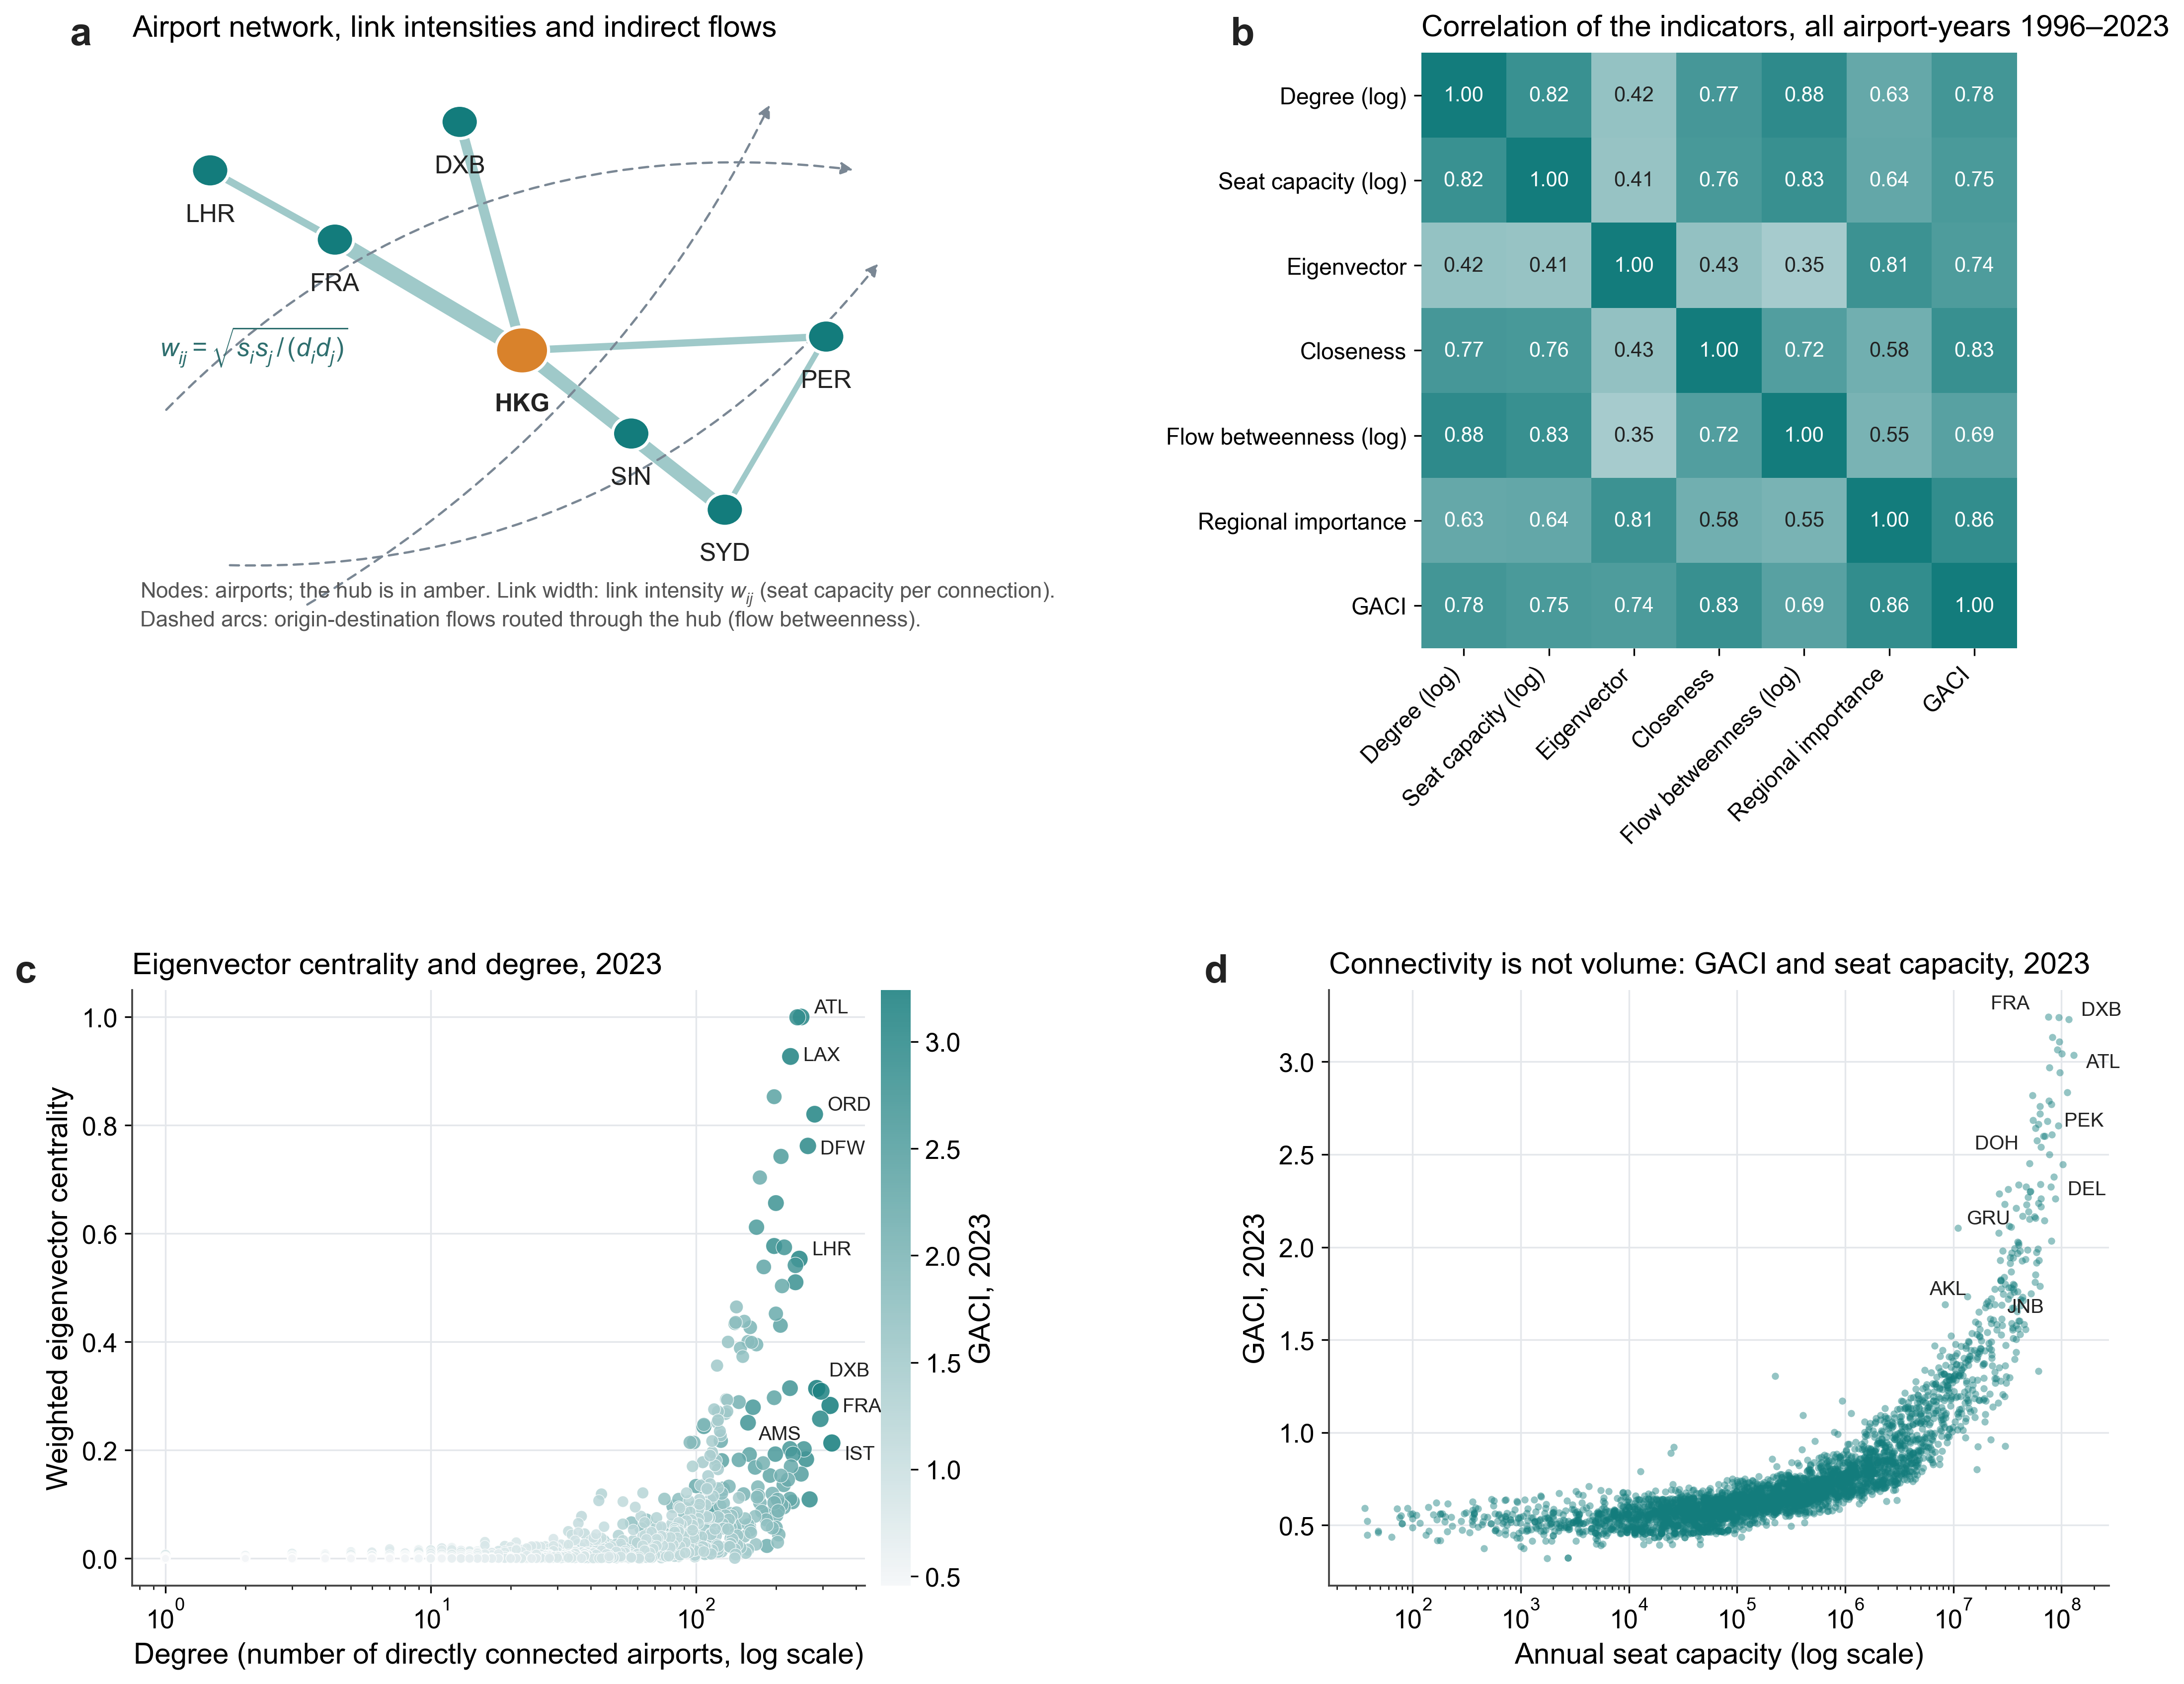
\includegraphics[width=\linewidth]{figures/FigB1_gaci_construction.png}
\caption{Construction of the connectivity index. (a) Schematic of the airport network: nodes are airports, the hub is in amber, link width is the link intensity $w_{ij}$, and dashed arcs are origin-destination flows routed through the hub. (b) Correlation matrix of the five indicators and the composite, all airport-years 1996--2023 (degree, seat capacity and flow betweenness in logs). (c) Weighted eigenvector centrality against degree, 2023, with colour and size proportional to GACI. (d) GACI against annual seat capacity, 2023. Source: authors' airport-year panel.}
\label{fig:construction}
\end{figure}

We aggregate the airport-level index to the country-year in three ways. Hub connectivity ($\mathrm{GACI}_{max}$) is the maximum across a country's airports, the connectivity of its primary gateway, and is the headline measure because the question of the paper concerns the hub. Hub quality ($\mathrm{GACI}_{cwm}$) is the seat-capacity-weighted mean, which uses the entire airport system while placing most weight on the dominant hubs. Total connectivity ($\mathrm{GACI}_{sum}$) is the sum across airports and blends hub connectivity with the size of the network. A fourth measure summarises the form of the network: the Gini coefficient of GACI across a country's airports, which is high where connectivity is concentrated in one gateway and low where it is spread across several airports. The three aggregations are on different scales and their coefficients are not comparable one for one; what we use is the pattern of signs and significance across them, and the difference between the hub and the sum, which identifies the network net of the hub.

\paragraph{Distributional outcomes}
The distribution of income comes from the World Inequality Database (WID), which provides the pretax national income of equal-split adults by decile, for the top 1 and 0.1 percent, and for the bottom 50 and middle 40 percent, together with post-tax national income shares for the bottom 50 and top 10 percent \citep{WID_2024}. The series are built on the distributional national accounts method of \citet{Piketty_2017}, which reconciles survey, tax and national-accounts data so that the group incomes sum to national income. Two properties of this construction are used throughout. First, the income share of a group is its average income times its population size divided by mean income, so the log share equals the log group income minus the log mean income up to a constant; the elasticity of a group's share is exactly the elasticity of its income minus the elasticity of mean income, and the elasticity of mean income is the share-weighted average of the group elasticities. Second, differences between group incomes can be entered as outcomes, which gives the difference of two elasticities with its standard error. From the decile data we form three groups that summarise the distribution: the bottom 30 percent (the first three deciles), the middle 40 percent (deciles four to seven), and the top 30 percent (deciles eight to ten). The grouping follows the data: as Section~\ref{sec:incidence} shows, the response of the distribution changes at the third decile. We also compute the Palma ratio, the absolute income gap between the top decile and the bottom half, and the Gini of the ten decile shares, and we use the survey-based market and disposable Gini coefficients of the Standardized World Income Inequality Database \citep{Solt_2020}, available for 166 of the economies, as a check in the appendix.

\paragraph{Instrument and other variables}
The instrument combines two components. The exposure is a country's air market access in the base year,
\begin{equation}
\mathrm{MA}^{air}_{c,1996} = \sum_{j \neq c} \frac{\mathrm{pop}_{j,1996}}{d^{air}_{cj}},
\label{eq:ma}
\end{equation}
where $d^{air}_{cj}$ is the great-circle distance in kilometres between the airport centroids of countries $c$ and $j$ (the mean coordinates of each country's airports with scheduled service) and the sum runs over every other country with population data, so that the measure is a gravity-weighted count of the world's population that can be reached by air, with the distance elasticity set to one as in \citet{Feyrer_2019}. It depends only on geography and on the 1996 distribution of world population. The shifter is a global aviation-intensity index $a_t$, the world's total scheduled seat capacity in the airline schedules of year $t$, min--max normalised to $[0,1]$ over 1996--2023, which tracks the world expansion of scheduled air service over the sample period. Their interaction, $Z_{ct}=a_t\times\ln\mathrm{MA}^{air}_{c,1996}$, is the Feyrer instrument described in Section~\ref{sec:strategy}. The maritime counterpart, $\mathrm{MA}^{sea}_{c,1996}$, replaces $d^{air}_{cj}$ with the port-to-port sea distance of the CERDI database and serves in the exclusion-restriction checks of Section~\ref{sec:robust}. Population and GDP per capita (constant 2015 US dollars) come from the World Development Indicators, as do the channel variables of Section~\ref{sec:mechanism}: industrial employment, urbanisation, trade relative to GDP, tourism receipts and international tourist arrivals. The composition of trade (the value of differentiated goods under the Rauch classification and of high value-to-weight goods) is computed from BACI. Neighbour definitions for the spillover analysis use land contiguity.

\paragraph{Sample and descriptive statistics}
The estimation sample is every country-year with WID decile incomes and a connectivity value: 178 economies and 4{,}537 country-years over 1996--2023. Table~\ref{tab:sumstat} reports summary statistics. Two features of the data matter for what follows. First, the distribution is slow moving: the within-country standard deviation of the bottom-30 share is half a point of national income against a cross-sectional standard deviation of two points. Second, hub connectivity also varies mainly across countries: its within standard deviation is 0.16 index units against 0.59 overall. Both features mean that the estimates rest on gradual within-country movements, and both explain why the inference reported below is clustered by country and, in robustness, allows for spatial correlation between countries.

\begin{table}[H]
\centering
\caption{Summary statistics, estimation sample (178 economies, 1996--2023).}
\label{tab:sumstat}
\begin{minipage}{\linewidth}
\centering
\resizebox{\linewidth}{!}{%
\begin{tabular}{lrrrrrr}
\toprule
Variable & N & Mean & SD & Within SD & Min & Max \\
\midrule
Top 30\% share of pretax income, \% & 4{,}537 & 70.442 & 7.298 & 2.030 & 50.660 & 86.740 \\
Middle 40\% (p30--70) share, \% & 4{,}537 & 24.339 & 5.443 & 1.566 & 11.310 & 40.830 \\
Bottom 30\% share, \% & 4{,}537 & 5.218 & 2.066 & 0.542 & 0.240 & 11.530 \\
Bottom 50\% share, \% & 4{,}537 & 14.826 & 4.537 & 1.241 & 5.070 & 27.930 \\
Top 10\% share, \% & 4{,}537 & 45.774 & 8.925 & 2.641 & 25.510 & 68.730 \\
Hub connectivity, GACI max & 4{,}537 & 1.264 & 0.587 & 0.155 & 0.534 & 3.626 \\
Hub quality, GACI cwm & 4{,}537 & 1.092 & 0.403 & 0.116 & 0.534 & 3.014 \\
Total connectivity, GACI sum & 4{,}537 & 14.579 & 42.351 & 5.755 & 0.545 & 510.036 \\
Gini of GACI across a country's airports & 3{,}659 & 0.119 & 0.057 & 0.020 & 0.000 & 0.374 \\
Population, millions & 4{,}537 & 40.216 & 146.076 & 13.041 & 0.011 & 1438.070 \\
GDP per capita, thousand constant 2015 US dollars & 4{,}537 & 13.905 & 19.305 & 3.426 & 0.227 & 118.383 \\
\bottomrule
\end{tabular}}
\par\vspace{3pt}\begin{flushleft}\footnotesize Within SD is the standard deviation after removing country means. Shares in percent of pretax national income (WID, equal-split adults); the WID group incomes that serve as outcomes are in constant local currency per adult and enter the regressions in logs, so their levels are not comparable across countries and are not tabulated. GACI in index units; the airport Gini is computed over the airports of each country-year (countries with at least two airports).\end{flushleft}
\end{minipage}
\end{table}


Figure~\ref{fig:maps} maps the geography of hub connectivity. Panel (a) plots every airport with scheduled service in 2023, with point size proportional to its index: the network is dense in North America, Europe and East Asia, and its largest nodes are the gateways of those regions together with Istanbul, Dubai, Jeddah and Singapore. Panel (b) aggregates to the country and shows the headline measure, $\ln\mathrm{GACI}_{max}$. Appendix Figure~\ref{fig:mapchange} maps the change in $\ln\mathrm{GACI}_{max}$ over the period, which is the variation the regressions use: hub connectivity rose most in Turkey, Korea, the Gulf, Ireland, Norway and much of South and East Asia, and fell in Russia, Ukraine, Venezuela and parts of Southern Africa. Figure~\ref{fig:airportgini} shows the form this growth took. The Gini of connectivity across a country's airports rose steadily over the period, and countries whose hubs grew most were also the countries in which connectivity became most concentrated: the correlation between the change in $\ln\mathrm{GACI}_{max}$ and the change in the airport Gini is $0.60$, and concentration rose in four fifths of the countries in which the hub grew. The connectivity growth of the past three decades was, in most countries, growth of a single gateway.

\begin{figure}[H]
\centering
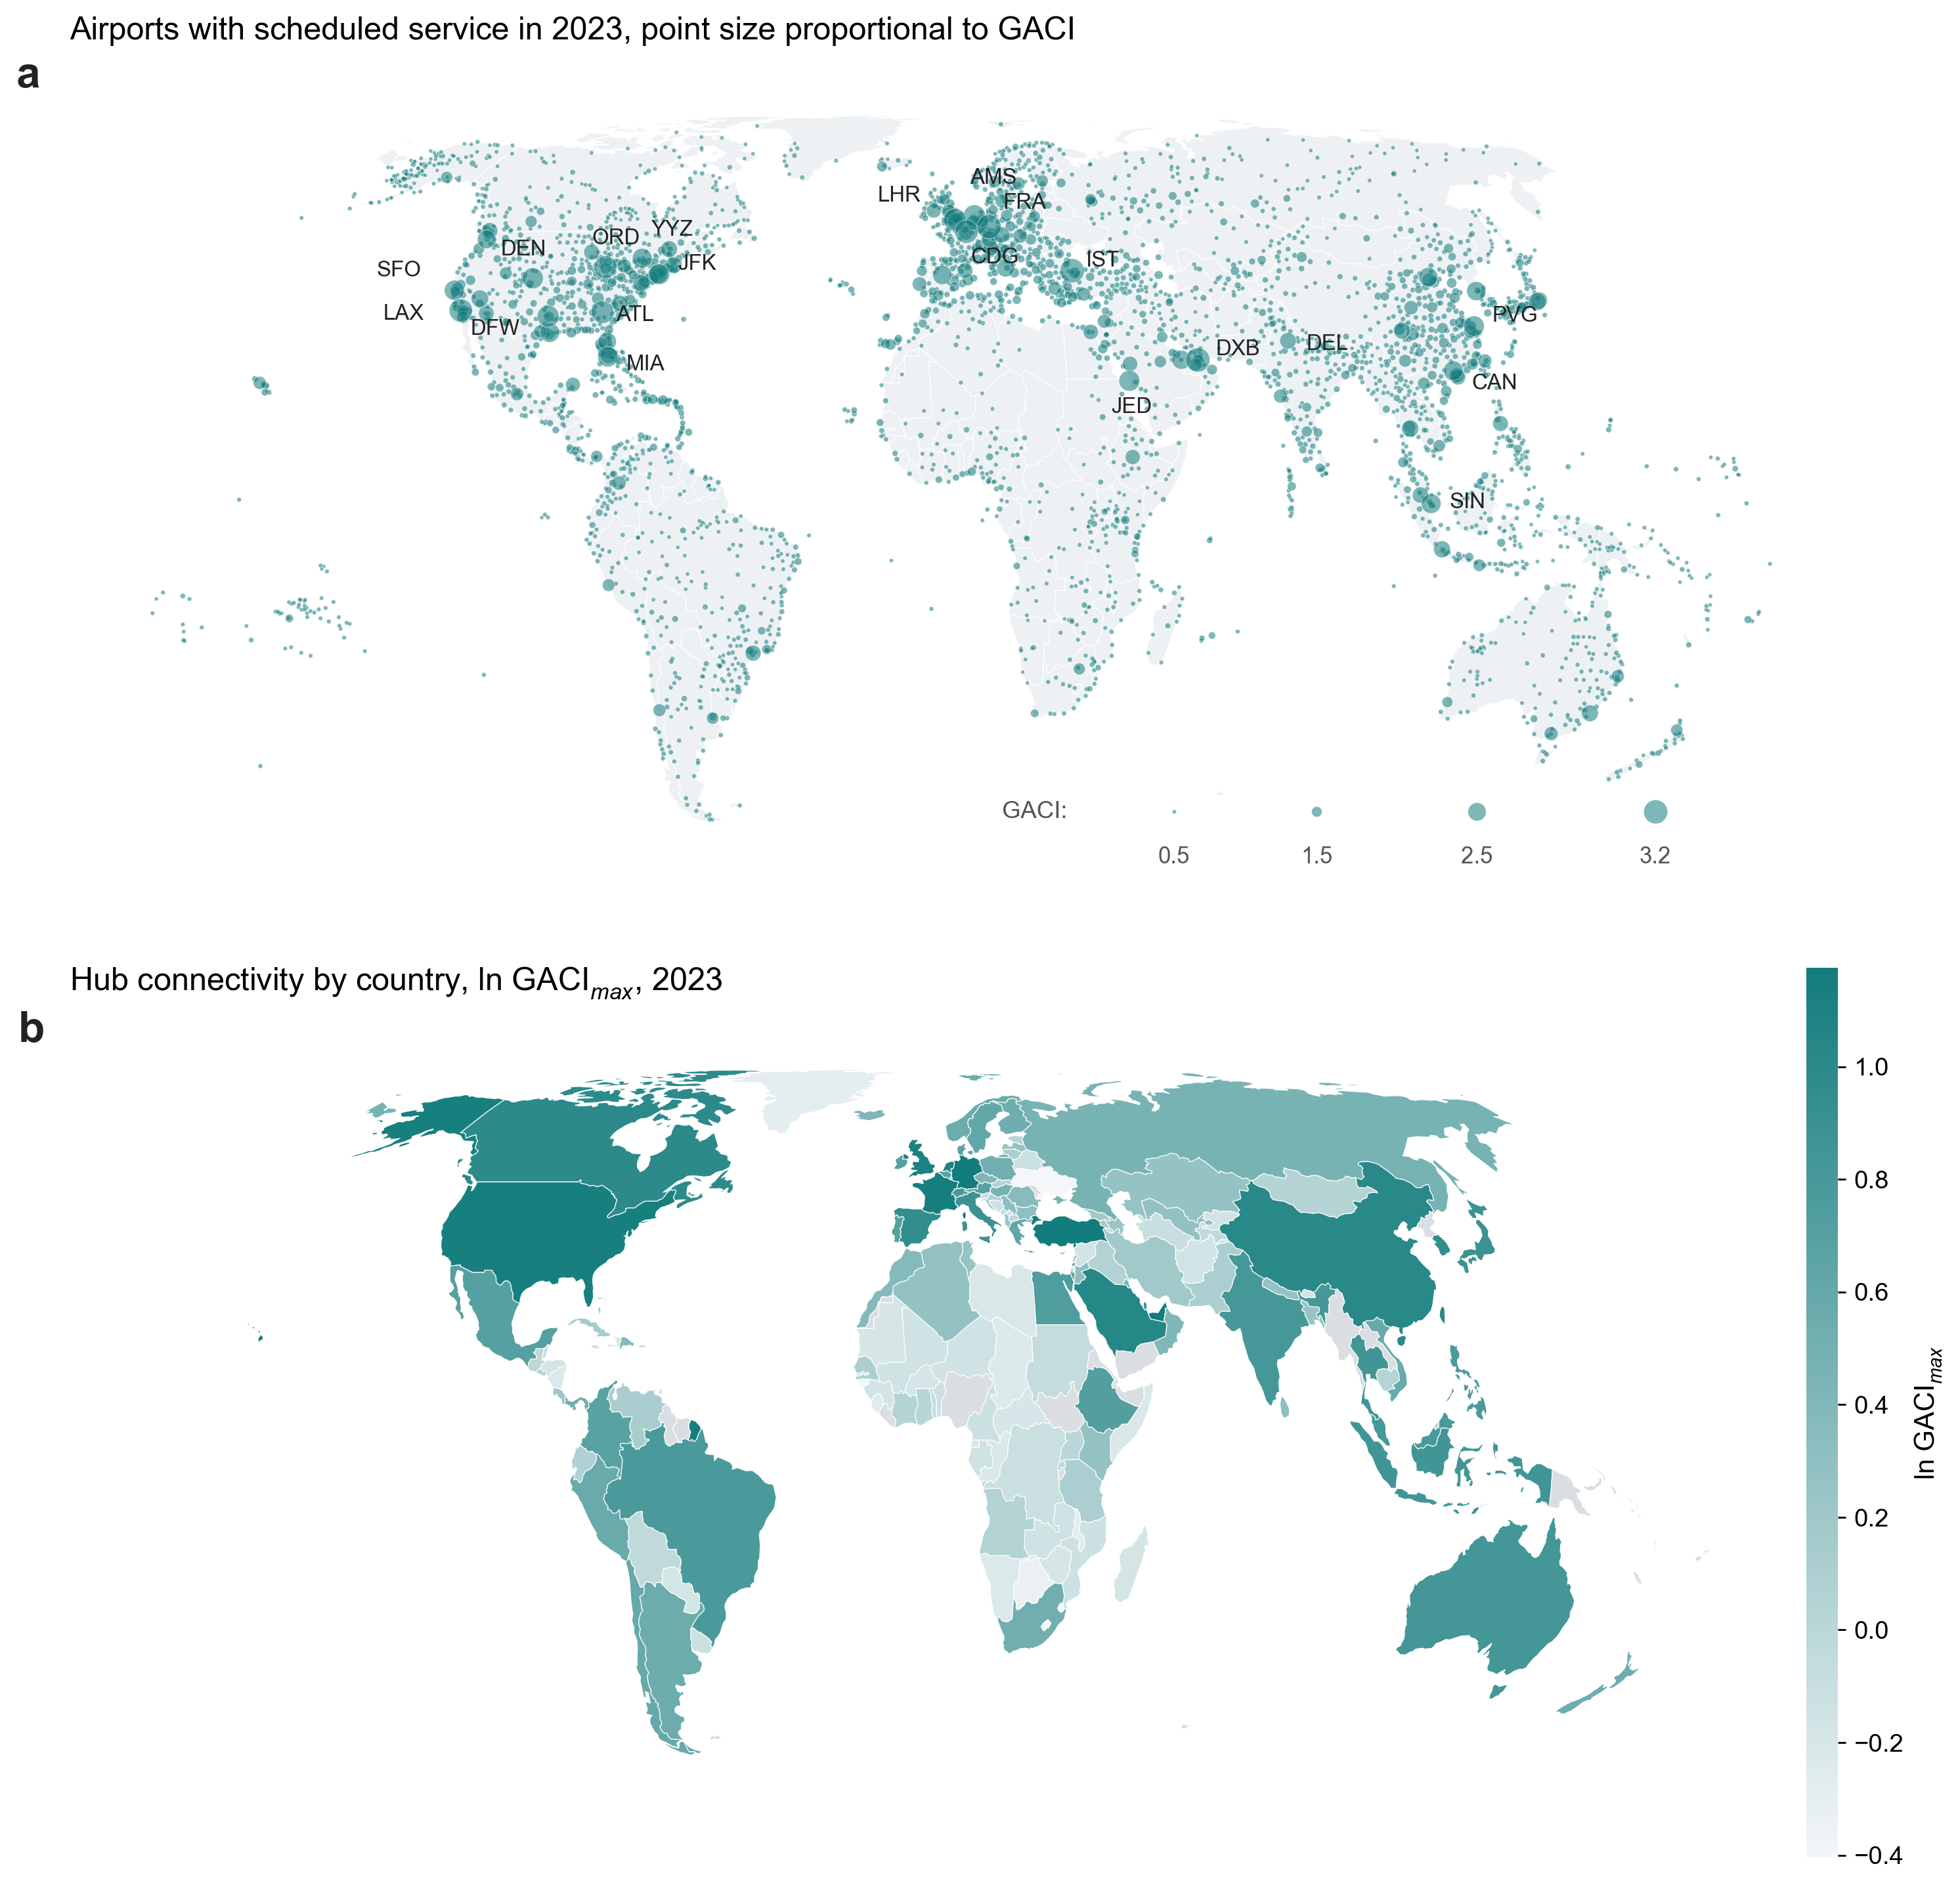
\includegraphics[width=0.92\linewidth]{figures/FigB3_maps_hubs.png}
\caption{The geography of hub connectivity, 2023. (a) Airports with scheduled service in 2023 (3{,}826 airports), point size proportional to GACI; the twenty most connected airports are labelled. (b) Hub connectivity by country, $\ln\mathrm{GACI}_{max}$, latest year; grey denotes economies outside the estimation sample. Equal Earth projection.}
\label{fig:maps}
\end{figure}

\begin{figure}[H]
\centering
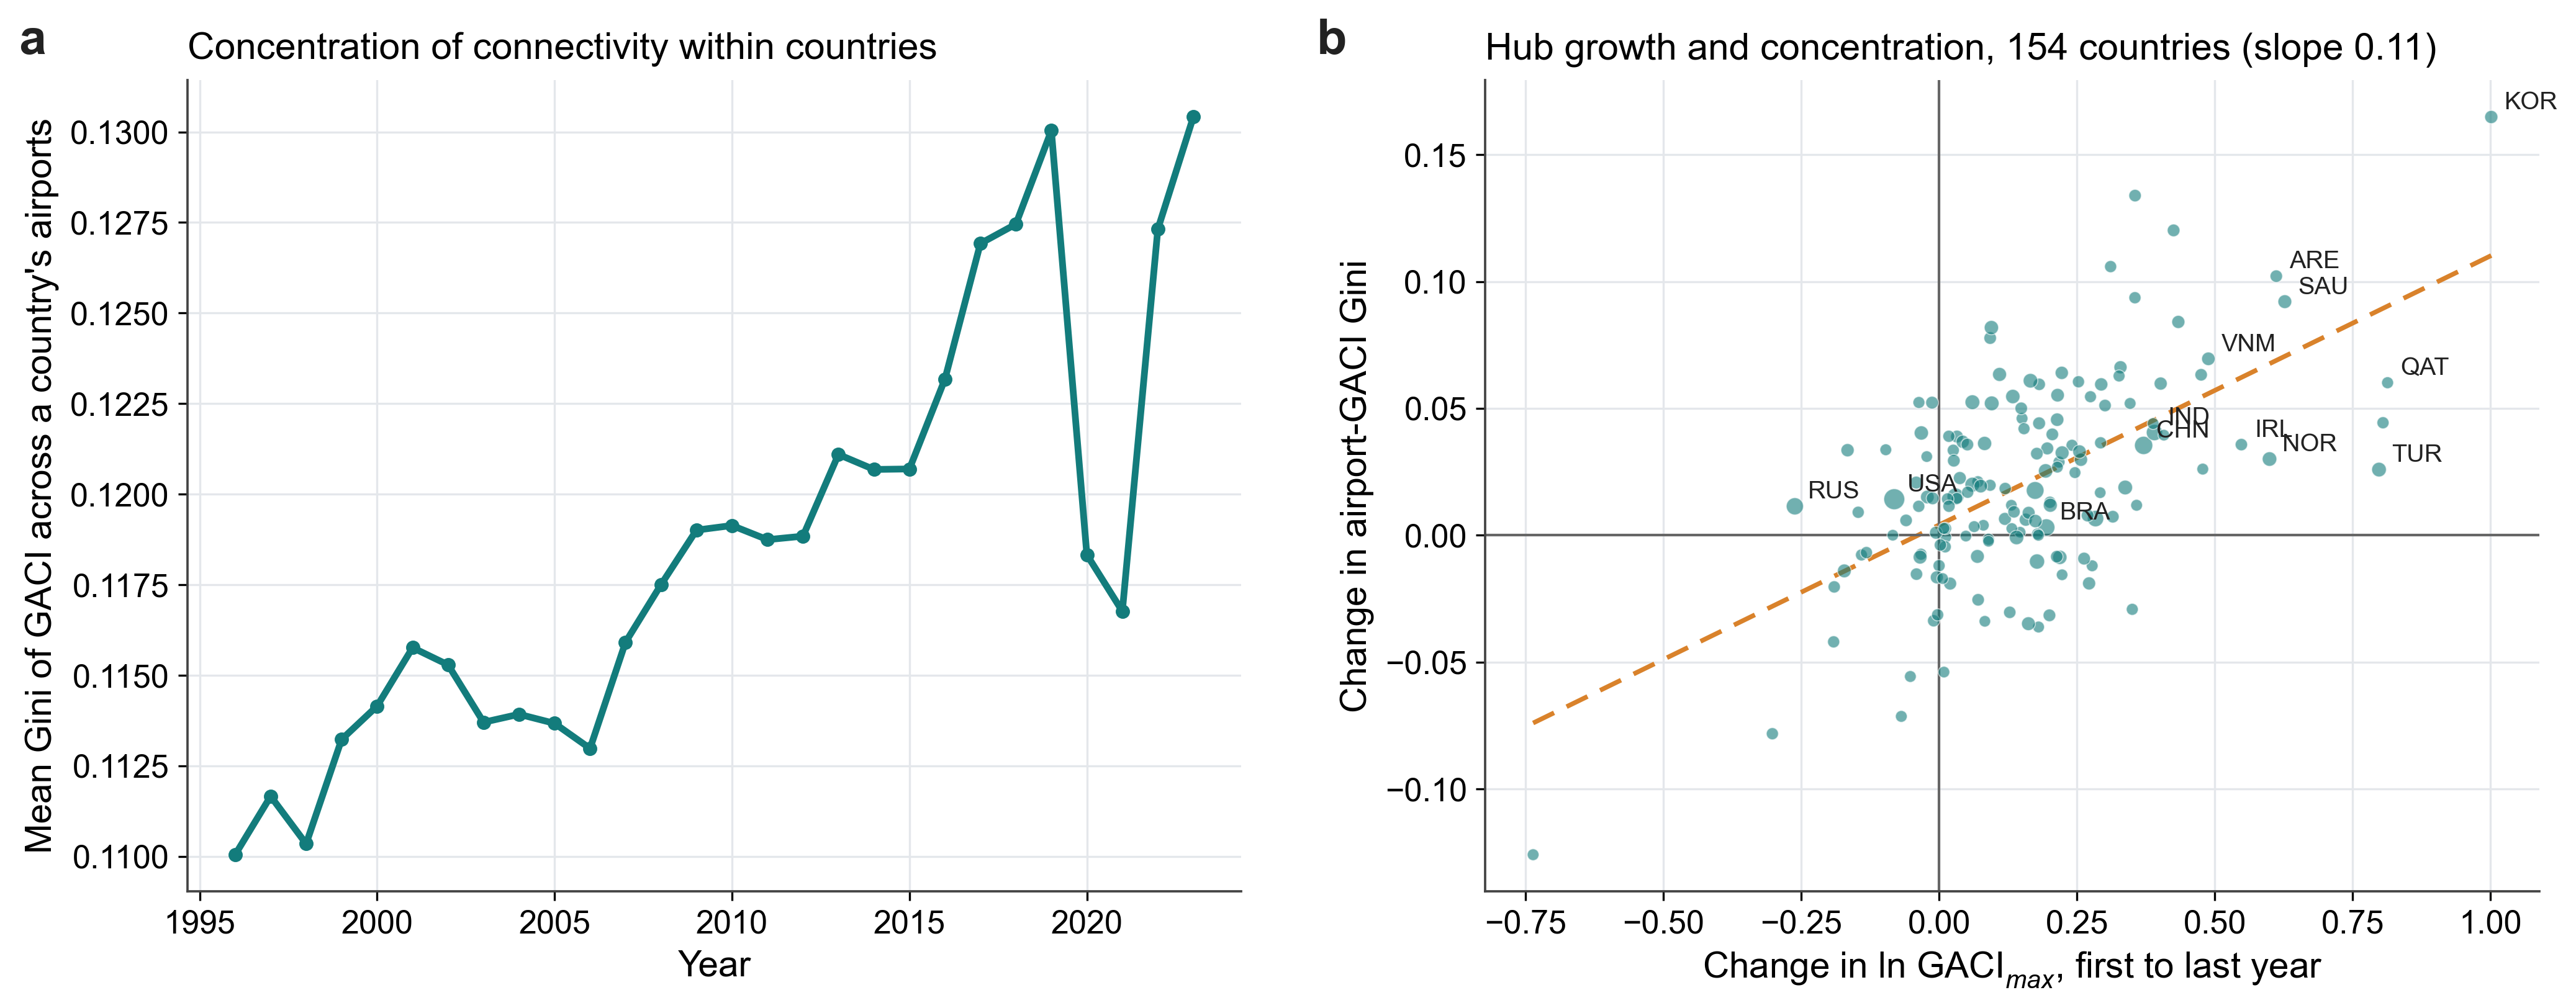
\includegraphics[width=\linewidth]{figures/FigB5_airport_gini.png}
\caption{Concentration of connectivity within countries. (a) Mean Gini of GACI across a country's airports, 1996--2023 (countries with at least two airports). (b) Change in the airport Gini against the change in $\ln\mathrm{GACI}_{max}$, first to last year, 154 countries; point size proportional to the number of airports; the dashed line is the fitted slope. Source: authors' airport-year panel.}
\label{fig:airportgini}
\end{figure}

\paragraph{A first look at incidence}
Before turning to the estimates, Figure~\ref{fig:descriptive} shows the raw pattern that motivates the paper. For the 162 countries of the estimation sample with at least fifteen years between their first and last observation, we compute the annualised growth of the average pretax income of each decile and group countries into terciles of the annualised growth of hub connectivity over the same window. Panel (a) plots the mean growth rate of each group for the high, middle and low connectivity-growth terciles, in the manner of the growth incidence curves of \citet{Ravallion_2003} and \citet{Alvaredo_2018}. Countries whose hubs grew fastest grew faster at every point of the distribution, but the gap rises with rank above the bottom: panel (b) shows that the high-minus-low difference is about 1.6 percentage points per year for the bottom decile, between 1.8 and 2.0 points from the third to the ninth decile, 2.1 points for the top decile and 2.4 points for the top percentile. The raw curve is descriptive and confounded by everything that moves both connectivity and growth; the rest of the paper asks whether the tilt survives a design that isolates exogenous variation in connectivity.

\begin{figure}[H]
\centering
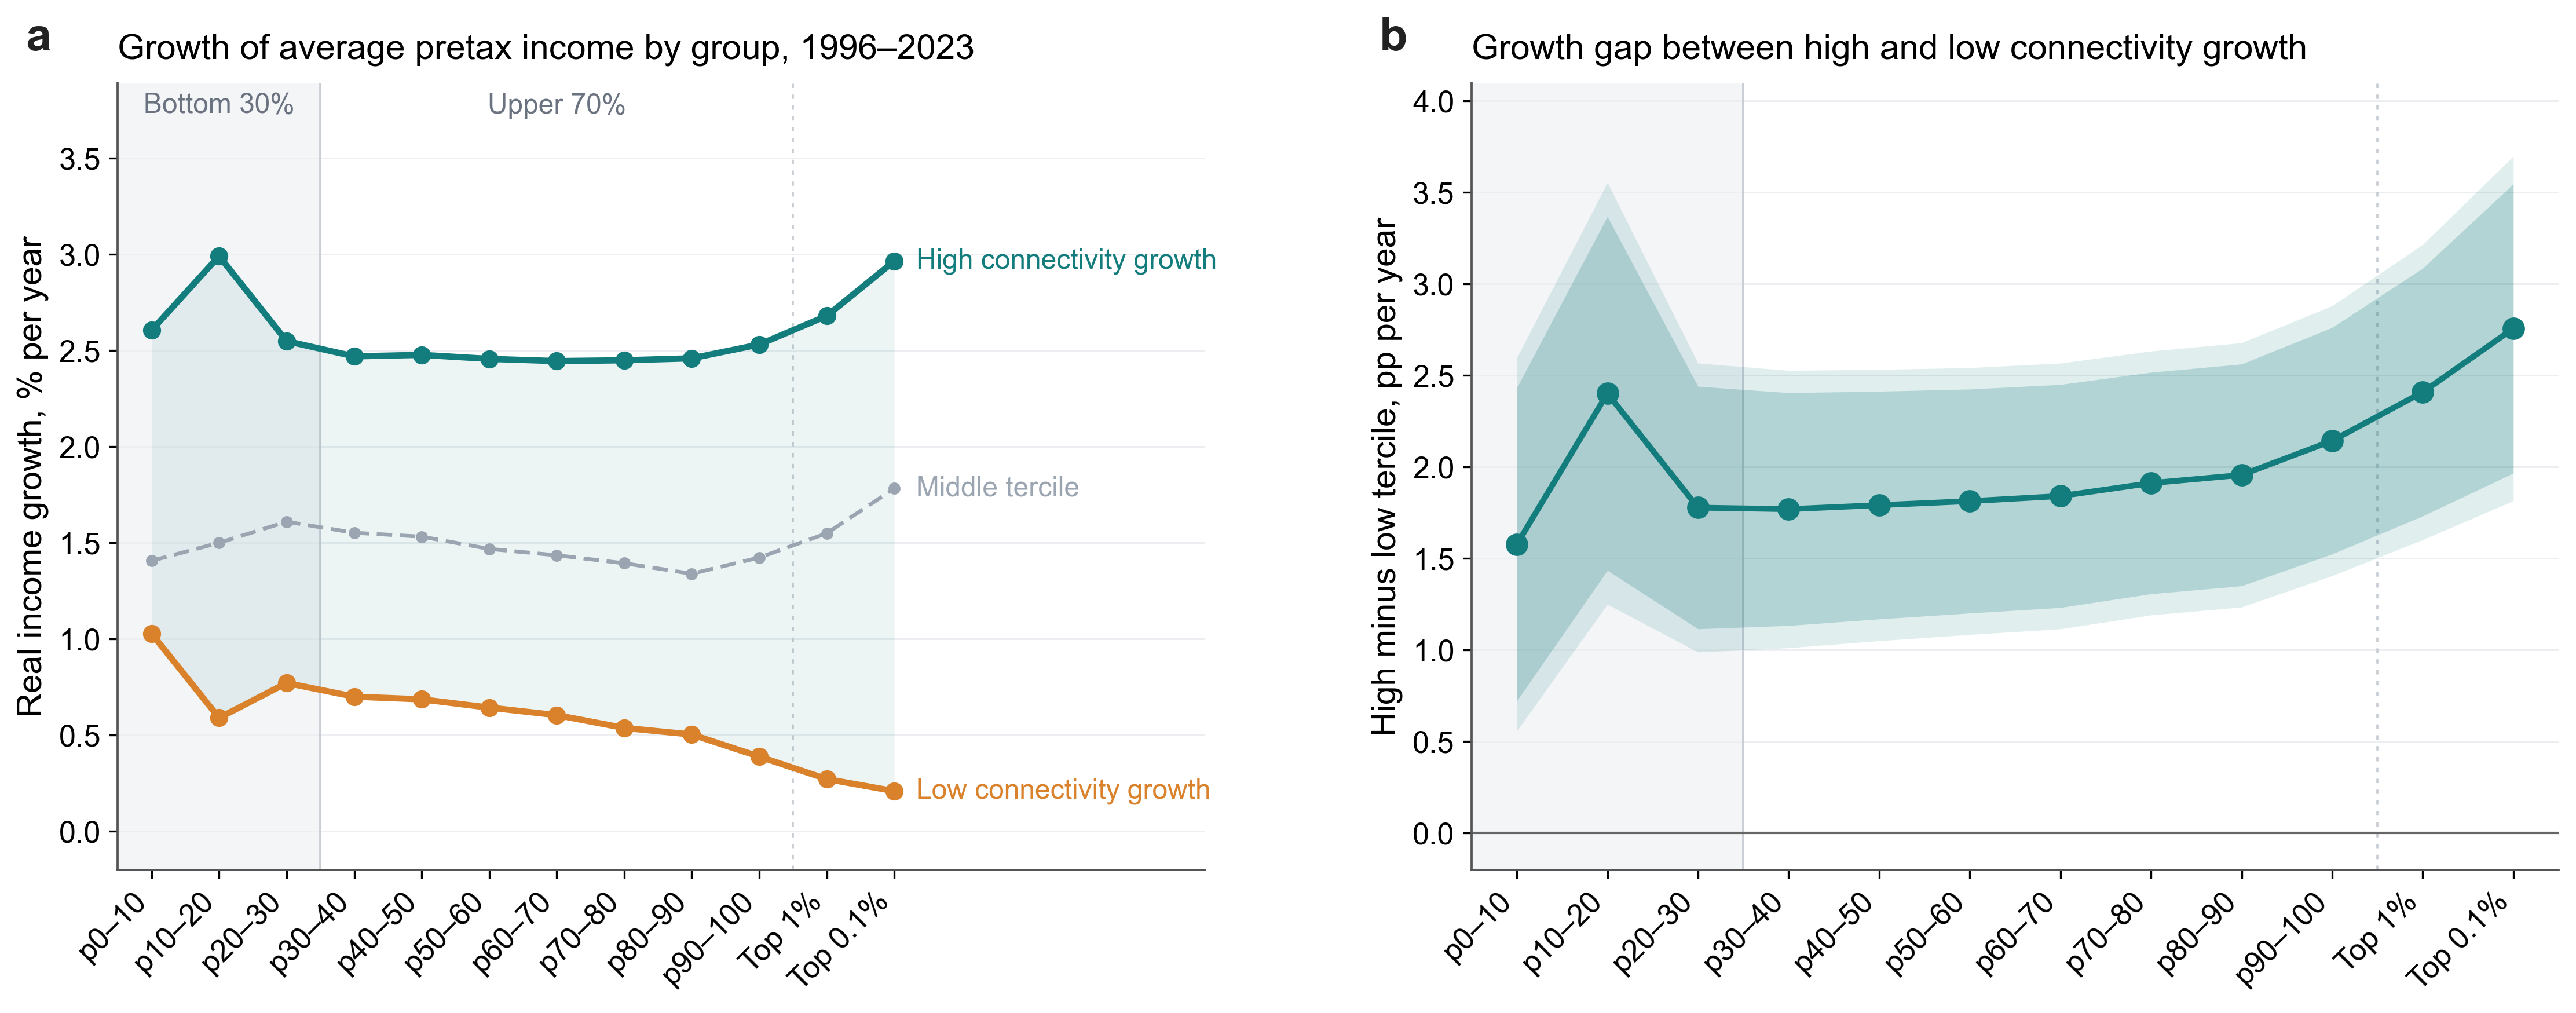
\includegraphics[width=\linewidth]{figures/FigW1_descriptive.png}
\caption{Descriptive growth incidence by hub-connectivity growth, 1996--2023. (a) Mean annualised real growth of average pretax income by WID group for countries in the high, middle and low terciles of annualised growth in $\ln\mathrm{GACI}_{max}$ (54 countries per tercile; the 162 countries of the estimation sample with at least fifteen years between their first and last observation); the shaded area between the high and low terciles is the growth gap. (b) Difference between the high and low terciles; the dark and light bands are 90 and 95 percent confidence intervals. The grey panel marks the bottom 30 percent of the distribution. Source: WID and authors' connectivity panel.}
\label{fig:descriptive}
\end{figure}

%=======================================================================
\section{Empirical strategy}
\label{sec:strategy}
%=======================================================================
To estimate the impact of hub connectivity on the distribution of income, we estimate the following model:
\begin{equation}
y_{ct} = \beta\,\ln\mathrm{GACI}_{ct} + \gamma\,\ln\text{pop}_{ct} + \alpha_c + \delta_t + \varepsilon_{ct},
\label{eq:main}
\end{equation}
where $y_{ct}$ is the natural logarithm of a distributional outcome of country $c$ in year $t$: the average pretax income of a group of the distribution, its income share, or the difference between two group incomes. $\ln\mathrm{GACI}_{ct}$ is the natural logarithm of hub connectivity ($\mathrm{GACI}_{max}$) in the headline specification, and of hub quality ($\mathrm{GACI}_{cwm}$) or total connectivity ($\mathrm{GACI}_{sum}$) in the alternatives. The model includes country fixed effects ($\alpha_c$) and year fixed effects ($\delta_t$). Population is the only time-varying control, for the same reason as in the companion papers: the country fixed effects absorb all time-invariant determinants of the distribution, and the natural time-varying candidates, GDP per capita, urbanisation, the sectoral structure and trade, are themselves outcomes of connectivity (Section~\ref{sec:mechanism}), so conditioning on them would control away part of the effect of interest. They enter instead as channels. Because $\beta$ is an elasticity, a coefficient of $-0.9$ on the bottom-30 share means that a 10 percent increase in hub connectivity lowers the share by 9 percent, or about half a point of national income at the sample mean of 5.2 percent.

Identifying the causal effect of connectivity on the distribution is difficult for two reasons. First, connectivity is poorly represented by a binary treatment. A country's hub gains connectivity continuously, through frequencies, partner growth and the growth of the partners' own networks, rather than through discrete, datable events; a continuous, network-based index that embeds partner-of-partner connections is the appropriate measurement. Second, the variation that does exist is endogenous: airlines add capacity where income is growing, and the reforms that attract them may also change the distribution of income directly. We therefore instrument connectivity with the Feyrer interaction
\begin{equation}
Z_{ct} = a_t \times \ln\mathrm{MA}^{air}_{c,1996},
\label{eq:iv}
\end{equation}
where $a_t$ is the global aviation-intensity index and $\mathrm{MA}^{air}_{c,1996}$ is the country's air market access in the base year \citep{Feyrer_2019}. The logic is that of \citet{Feyrer_2019}: as aviation expanded worldwide, countries whose geography placed them nearer, by air, to the rest of the world's population gained connectivity by more, for reasons that have nothing to do with their own income distribution. The instrument has the shift-share structure of \citet{GoldsmithPinkham_2020}, \citet{Adao_2019} and \citet{Borusyak_2022} with a single global shifter and a predetermined exposure. Country fixed effects absorb the exposure, year fixed effects absorb the shifter, and identification rests on their interaction alone. The identifying assumption is that, conditional on the fixed effects, countries with higher baseline air market access did not experience differential distributional trends for reasons other than connectivity.

The exclusion restriction deserves to be stated in terms of the threats to it. The shifter is global and the exposure is a fixed geographic characteristic, so the instrument can fail only if some other global trend over 1996--2023 benefited countries in proportion to their air market access and affected the distribution of income directly. Three candidates are plausible. The first is trade globalisation: a country near the world's population by air is also near it by sea, and the expansion of maritime trade over the period could have changed the distribution through the channels the trade literature identifies. This is the threat \citet{Feyrer_2019} addresses by separating air from sea distance, and we follow him: the maritime market access $\mathrm{MA}^{sea}_{c,1996}$ of Equation~\eqref{eq:ma}, interacted with the same shifter, is added as a control, so that identification comes from the component of air market access that sea market access does not share. The second is convergence: countries that were poorer or larger in 1996 may have followed different distributional paths over the period for reasons unrelated to aviation, and if income or size correlates with air market access the instrument would pick them up; we add the interactions of baseline GDP per capita and of land area with the shifter. The third is reverse timing, that airlines add capacity where incomes are already growing; this is the endogeneity the instrument is designed to remove, since the shifter is world capacity rather than the country's own. Section~\ref{sec:robust} reports the estimates under each control. The instrument also requires that the base-year exposure not be an outcome of the distribution; air market access in 1996 is a function of other countries' population and of distance, neither of which a country's income distribution affects.

The first-stage regression is
\begin{equation}
\ln\mathrm{GACI}_{ct} = \pi_1 Z_{ct} + \pi_2 \ln\text{pop}_{ct} + \mu_c + \lambda_t + \nu_{ct},
\label{eq:first}
\end{equation}
and the second stage replaces $\ln\mathrm{GACI}_{ct}$ in Equation~\eqref{eq:main} with its fitted value. We report the Kleibergen--Paap $rk$ Wald statistic (KP $F$) for every 2SLS estimate; in the full sample it is $21.1$. Because the distribution and connectivity are both persistent and move slowly, the errors of Equation~\eqref{eq:main} are serially correlated within countries, and we cluster standard errors by country throughout. Countries are also spatially dependent, so in robustness we report Conley standard errors \citep{Conley_1999} with a Bartlett kernel in great-circle distance between country centroids at cutoffs of 1{,}000 and 2{,}000 km, allowing arbitrary within-country serial correlation, and two-way clustering by country and year. For the split-sample estimates, whose first stages are weaker, we also report the $p$-value of the instrument in the reduced form, which does not depend on first-stage strength.

For additional analyses, we examine (1) the incidence of connectivity across the income distribution, (2) growth and its incidence by baseline hub size, (3) the mechanisms through which hub connectivity acts on the distribution, and (4) the aggregate contribution of connectivity growth to the distribution over 1996--2023.

For (1), we estimate Equation~\eqref{eq:main} separately for the log average pretax income of each WID group $g$ (ten deciles, the top 1 and top 0.1 percent, the bottom 50 and the middle 40 percent, and the bottom 30, middle 40 and top 30 percent) and for its log income share. Because the WID groups exhaust national income, the log income share is the log group income minus the log mean income of all adults, so the share elasticity is the group elasticity minus the mean-income elasticity, and all groups are estimated on the same sample. The set of group elasticities plotted against rank is the instrumented counterpart of the growth incidence curve \citep{Ravallion_2003}. To test differences between groups exactly, we regress the difference of two group outcomes (for example, the log income of the top 30 percent minus the log income of the bottom 30 percent) on instrumented connectivity, which gives the difference of the two elasticities with its standard error.

For (2), we ask whether connectivity raises income and changes its distribution together, and where. We split countries on their baseline hub connectivity ($\mathrm{GACI}_{max}$ in 1996 or the earliest observed year) at the median and into terciles and estimate Equation~\eqref{eq:main} by 2SLS within each group for GDP per capita, mean income, the income and share of the bottom 30 percent and the top-30-minus-bottom-30 gap. We use split samples rather than an interaction model because the instrument's power differs sharply across groups: the Feyrer interaction moves the connectivity of hubs that are integrating into the network and has little purchase on hubs that were already among the world's largest in 1996. Reporting the first-stage statistic for each group makes this visible, and we interpret only groups in which the instrument has power.

For (3), we ask five questions, each with a regression. First, which connectivity carries the pattern: we enter hub connectivity together with total connectivity or with the connectivity of the country's other airports as a control, and we instrument the hub's eigenvector centrality while controlling for its seat capacity. Second, who gains: the incidence regressions of (1). Third, whether the growth channels that connectivity opens transmit the effect: for a channel variable $\mathrm{M}_{ct}$ (GDP per capita, differentiated-goods trade, high value-to-weight trade, tourist arrivals, industrial employment) we estimate
\begin{equation}
\mathrm{M}_{ct} = a\,\ln\mathrm{GACI}_{ct} + \kappa\,\ln\text{pop}_{ct} + \xi_c + \zeta_t + \phi_{ct},
\label{eq:mec1}
\end{equation}
\begin{equation}
y_{ct} = \beta^{d}\,\ln\mathrm{GACI}_{ct} + \theta\,\mathrm{M}_{ct} + \gamma\,\ln\text{pop}_{ct} + \alpha_c + \delta_t + \varepsilon_{ct},
\label{eq:mec2}
\end{equation}
with connectivity instrumented in both equations and $\mathrm{M}_{ct}$ entered in the second stage of Equation~\eqref{eq:mec2} as a control. The total effect of Equation~\eqref{eq:main} then decomposes exactly into a direct and a transmitted part, $\beta=\beta^{d}+a\theta$, when both are estimated on the channel's sample: $\beta^{d}$ is the effect of the hub with the channel held fixed and $a\theta$ is the part that runs through the connectivity-induced change in $\mathrm{M}$, in the manner of the covariate decomposition of \citet{Gelbach_2016}. Because $\mathrm{M}_{ct}$ is itself an outcome of connectivity and a single instrument is used, $\theta$ is identified only under the assumption that the channel coefficient is not confounded, so we present the decomposition as a descriptive accounting rather than as causal mediation. What it can show is whether the exclusion of the bottom survives, shrinks or grows when the growth that connectivity generates is held fixed. Fourth, where the pattern is found: split samples by the concentration of the airport network, urbanisation, baseline income, tourism dependence and era, and a spillover regression in which own connectivity and the leave-out mean of contiguous neighbours' connectivity enter jointly, each instrumented by its own shifter. Fifth, whether redistribution offsets the outcome: the pretax and post-tax shares of the bottom 50 and top 10 percent, and their difference.

For (4), we quantify the aggregate contribution of connectivity growth by multiplying each country's observed change in $\ln\mathrm{GACI}_{max}$ between its first and last year with data by the 2SLS elasticities for mean income and for the income and share of each group, and aggregating across countries with and without population weights (Section~\ref{sec:aggregate}).

%=======================================================================
\section{Main results}
\label{sec:results}
%=======================================================================
\subsection{Hub connectivity, income and the bottom of the distribution}
\label{sec:headline}
We first ask whether hub connectivity raised income and where the income arrived. Table~\ref{tab:main} reports, for each of our three measures of connectivity, three lines side by side: the first-stage relevance of the instrument, the OLS association, and the instrumented (2SLS) estimate, for five outcomes that summarise the distribution: mean income, the average income of the top 30 percent, the average income of the bottom 30 percent, the bottom-30 share, and the gap between the top and bottom 30 percent. Reading down each panel shows how isolating exogenous variation changes the picture. The three measures agree in sign and significance, and we adopt hub connectivity ($\ln\mathrm{GACI}_{max}$) as the headline because the hypotheses concern the hub; hub quality and total connectivity serve as robustness measures and, in Section~\ref{sec:mechanism}, to separate the hub from the network.

\begin{table}[H]
\centering
\caption{Main results: OLS, first stage, and 2SLS, by connectivity measure.}
\label{tab:main}
\begin{minipage}{\linewidth}
\centering
\resizebox{\linewidth}{!}{%
\begin{tabular}{lccccc}
\toprule
 & Mean income & Top-30\% income & Bottom-30\% income & Bottom-30\% share & Top-30 minus bottom-30 \\
 & $\ln y$ & $\ln y_{70-100}$ & $\ln y_{0-30}$ & $\ln s_{0-30}$ & $\ln y_{70-100}-\ln y_{0-30}$ \\
\midrule
\multicolumn{6}{l}{\emph{Panel A. Hub connectivity, $\ln\mathrm{GACI}_{max}$ (headline)}}\\
First stage: instrument coef. & \multicolumn{5}{l}{0.163\sym{***}\ \ (0.036),\ \ KP $F=21.1$} \\
OLS & 0.731\sym{***} & 0.752\sym{***} & 0.728\sym{***} & -0.003 & 0.023 \\
 & (0.122) & (0.117) & (0.148) & (0.065) & (0.084) \\
2SLS & 1.320\sym{***} & 1.361\sym{***} & 0.410 & -0.910\sym{*} & 0.951\sym{*} \\
 & (0.420) & (0.415) & (0.631) & (0.498) & (0.573) \\
\addlinespace
\multicolumn{6}{l}{\emph{Panel B. Hub quality, $\ln\mathrm{GACI}_{cwm}$}}\\
First stage: instrument coef. & \multicolumn{5}{l}{0.140\sym{***}\ \ (0.033),\ \ KP $F=18.6$} \\
OLS & 0.761\sym{***} & 0.773\sym{***} & 0.811\sym{***} & 0.050 & -0.038 \\
 & (0.129) & (0.126) & (0.156) & (0.073) & (0.093) \\
2SLS & 1.539\sym{***} & 1.586\sym{***} & 0.477 & -1.061\sym{*} & 1.108 \\
 & (0.498) & (0.491) & (0.735) & (0.587) & (0.673) \\
\addlinespace
\multicolumn{6}{l}{\emph{Panel C. Total connectivity, $\ln\mathrm{GACI}_{sum}$}}\\
First stage: instrument coef. & \multicolumn{5}{l}{0.306\sym{***}\ \ (0.083),\ \ KP $F=13.5$} \\
OLS & 0.179\sym{***} & 0.180\sym{***} & 0.173\sym{***} & -0.006 & 0.007 \\
 & (0.032) & (0.032) & (0.038) & (0.018) & (0.023) \\
2SLS & 0.704\sym{***} & 0.725\sym{***} & 0.218 & -0.485\sym{*} & 0.507\sym{*} \\
 & (0.264) & (0.264) & (0.346) & (0.265) & (0.305) \\
\addlinespace
\midrule
Country, Year FE & Yes & Yes & Yes & Yes & Yes \\
Observations & 4{,}537 & 4{,}537 & 4{,}537 & 4{,}537 & 4{,}537 \\
\bottomrule
\end{tabular}}
\par\vspace{3pt}\begin{flushleft}\footnotesize Each panel instruments its connectivity measure with the Feyrer interaction. The first-stage row regresses the connectivity measure on the instrument with log population and two-way fixed effects. The last column is a difference outcome and gives the exact difference of the two elasticities with its standard error. Country-year panel of 178 economies, 1996--2023. All regressions include country and year fixed effects and log population. 2SLS instruments $\ln\mathrm{GACI}_{max}$ with the Feyrer interaction $Z_{ct}=a_t\times\ln\mathrm{MA}^{air}_{c,1996}$; KP $F$ is the Kleibergen--Paap $rk$ Wald statistic. Group incomes are the log average pretax national income of the group (WID, equal-split adults); shares are log income shares, computed as log group income minus log mean income so that all groups use the same sample. Standard errors clustered by country in parentheses. \sym{*}~$p<0.10$, \sym{**}~$p<0.05$, \sym{***}~$p<0.01$.\end{flushleft}
\end{minipage}
\end{table}


Panel A uses hub connectivity. The instrument is a strong predictor of connectivity: it enters the first stage with the expected positive sign ($0.163$, $p<0.01$) and a Kleibergen--Paap statistic of $21.1$. In OLS, a one percent increase in hub connectivity is associated with a $0.73$ percent increase in mean income, and the association is the same for the top and the bottom 30 percent, so that the bottom-30 share does not move ($-0.003$). The 2SLS estimates separate the groups. Mean income rises with an elasticity of $1.32$ ($p<0.01$) and the income of the top 30 percent with an elasticity of $1.36$ ($p<0.01$), but the income of the bottom 30 percent does not respond ($0.41$, standard error $0.63$). The bottom-30 share therefore falls, with an elasticity of $-0.91$ ($p<0.10$), and the gap between the top and bottom 30 percent widens by $0.95$ ($p<0.10$). A coefficient of $-0.91$ means that a 10 percent increase in hub connectivity lowers the share of the bottom 30 percent by about 9 percent, or half a point of national income at the sample mean of 5.2 percent; one within-country standard deviation of hub connectivity, about 12 percent of the mean, lowers it by 0.6 points, which is more than the within-country standard deviation of the share itself. These estimates bear directly on \textbf{Hypothesis~1}, which predicts that hub connectivity increases mean income, and \textbf{Hypothesis~1} is supported. They also give the first evidence on \textbf{Hypothesis~2}: the income reaches the top of the distribution and not its bottom.

That the 2SLS estimate for mean income exceeds the OLS estimate is consistent with measurement error in a composite index and with the timing of airline capacity, which follows income with a lag so that contemporaneous OLS understates the response; the instrument isolates the variation in connectivity that arrives through the global network. That the 2SLS estimates for the top and the bottom diverge while the OLS estimates do not is the substantive finding: the connectivity that a country acquires through the world's expansion of aviation is received by the upper part of its distribution.

Panel B uses hub quality ($\ln\mathrm{GACI}_{cwm}$), the capacity-weighted mean across the airport system, and Panel C total connectivity ($\ln\mathrm{GACI}_{sum}$). The signs and significance carry over: mean income rises with elasticities of $1.54$ and $0.70$ (both $p<0.01$), the bottom-30 income does not respond, and the bottom-30 share falls with elasticities of $-1.06$ and $-0.49$ (both $p<0.10$). The first stage is weaker for the sum ($F=13.5$) because the sum blends the hub with the rest of the network. The three measures are on different scales and cannot be compared coefficient for coefficient; what carries over is the common pattern, so that the support for \textbf{Hypothesis~1} and the first evidence on \textbf{Hypothesis~2} are not artefacts of any one aggregation of connectivity.

%=======================================================================
\subsection{Incidence across the income distribution}
\label{sec:incidence}
The three-group summary hides where the distribution divides, so we next ask which deciles move. Table~\ref{tab:incidence} and Figure~\ref{fig:incidence} report the 2SLS elasticity of the average pretax income of each WID group (left columns) and of its income share (right columns) to hub connectivity; each cell is a separate regression on the same sample of 4{,}537 country-years (4{,}534 and 4{,}536 for the two lowest deciles, whose average income is undefined where it is non-positive), so the coefficients are directly comparable across rows.

\begin{table}[p]
\centering
\caption{Incidence of hub connectivity across the income distribution (2SLS, Feyrer instrument).}
\label{tab:incidence}
\begin{threeparttable}
\small
\begin{tabular}{lcccc}
\toprule
 & \multicolumn{2}{c}{Average income of the group} & \multicolumn{2}{c}{Income share of the group} \\
\cmidrule(lr){2-3}\cmidrule(lr){4-5}
WID group & Coef. & (s.e.) & Coef. & (s.e.) \\
\midrule
\multicolumn{5}{l}{\emph{Panel A. Elasticity to $\ln\mathrm{GACI}_{max}$, 2SLS}}\\
p0--10 & 0.245 & (1.167) & -1.073 & (1.050) \\
p10--20 & -0.677 & (1.375) & -1.995 & (1.346) \\
p20--30 & 0.590 & (0.575) & -0.730\sym{*} & (0.416) \\
p30--40 & 0.974\sym{*} & (0.523) & -0.346 & (0.290) \\
p40--50 & 1.073\sym{**} & (0.498) & -0.247 & (0.246) \\
p50--60 & 1.195\sym{**} & (0.486) & -0.125 & (0.201) \\
p60--70 & 1.275\sym{***} & (0.474) & -0.045 & (0.157) \\
p70--80 & 1.346\sym{***} & (0.461) & 0.026 & (0.118) \\
p80--90 & 1.363\sym{***} & (0.448) & 0.043 & (0.091) \\
p90--100 & 1.381\sym{***} & (0.418) & 0.061 & (0.165) \\
Top 1\% & 1.359\sym{***} & (0.445) & 0.039 & (0.297) \\
Top 0.1\% & 0.924\sym{*} & (0.546) & -0.396 & (0.483) \\
Bottom 30\% & 0.410 & (0.631) & -0.910\sym{*} & (0.498) \\
Middle 40\% (p30--70) & 1.166\sym{**} & (0.487) & -0.154 & (0.206) \\
Top 30\% & 1.361\sym{***} & (0.415) & 0.041 & (0.093) \\
Bottom 50\% & 0.901\sym{*} & (0.526) & -0.419 & (0.309) \\
All adults (mean income) & 1.320\sym{***} & (0.420) & -- &  \\
\addlinespace
\multicolumn{5}{l}{\emph{Panel B. Differences between groups (difference outcomes)}}\\
Top 30\% minus bottom 30\% & 0.951\sym{*} & (0.573) & & \\
Top half minus bottom half & 0.452 & (0.354) & & \\
p90--100 minus bottom 50\% & 0.481 & (0.462) & & \\
Top 1\% minus p90--100 & -0.022 & (0.186) & & \\
\midrule
First-stage KP $F$ & \multicolumn{2}{c}{21.1} & \multicolumn{2}{c}{21.1} \\
Observations & \multicolumn{2}{c}{4{,}537} & \multicolumn{2}{c}{4{,}537} \\
\bottomrule
\end{tabular}
\begin{tablenotes}\small
\item Each cell is a separate regression on the same sample; the average income of the bottom two deciles is undefined (non-positive) in 3 and 1 country-years, so those rows use 4{,}534 and 4{,}536 observations. Panel B regresses the difference of two group outcomes on instrumented connectivity. Country-year panel of 178 economies, 1996--2023. All regressions include country and year fixed effects and log population. 2SLS instruments $\ln\mathrm{GACI}_{max}$ with the Feyrer interaction $Z_{ct}=a_t\times\ln\mathrm{MA}^{air}_{c,1996}$; KP $F$ is the Kleibergen--Paap $rk$ Wald statistic. Group incomes are the log average pretax national income of the group (WID, equal-split adults); shares are log income shares, computed as log group income minus log mean income so that all groups use the same sample. Standard errors clustered by country in parentheses. \sym{*}~$p<0.10$, \sym{**}~$p<0.05$, \sym{***}~$p<0.01$.
\end{tablenotes}
\end{threeparttable}
\end{table}


\begin{figure}[H]
\centering
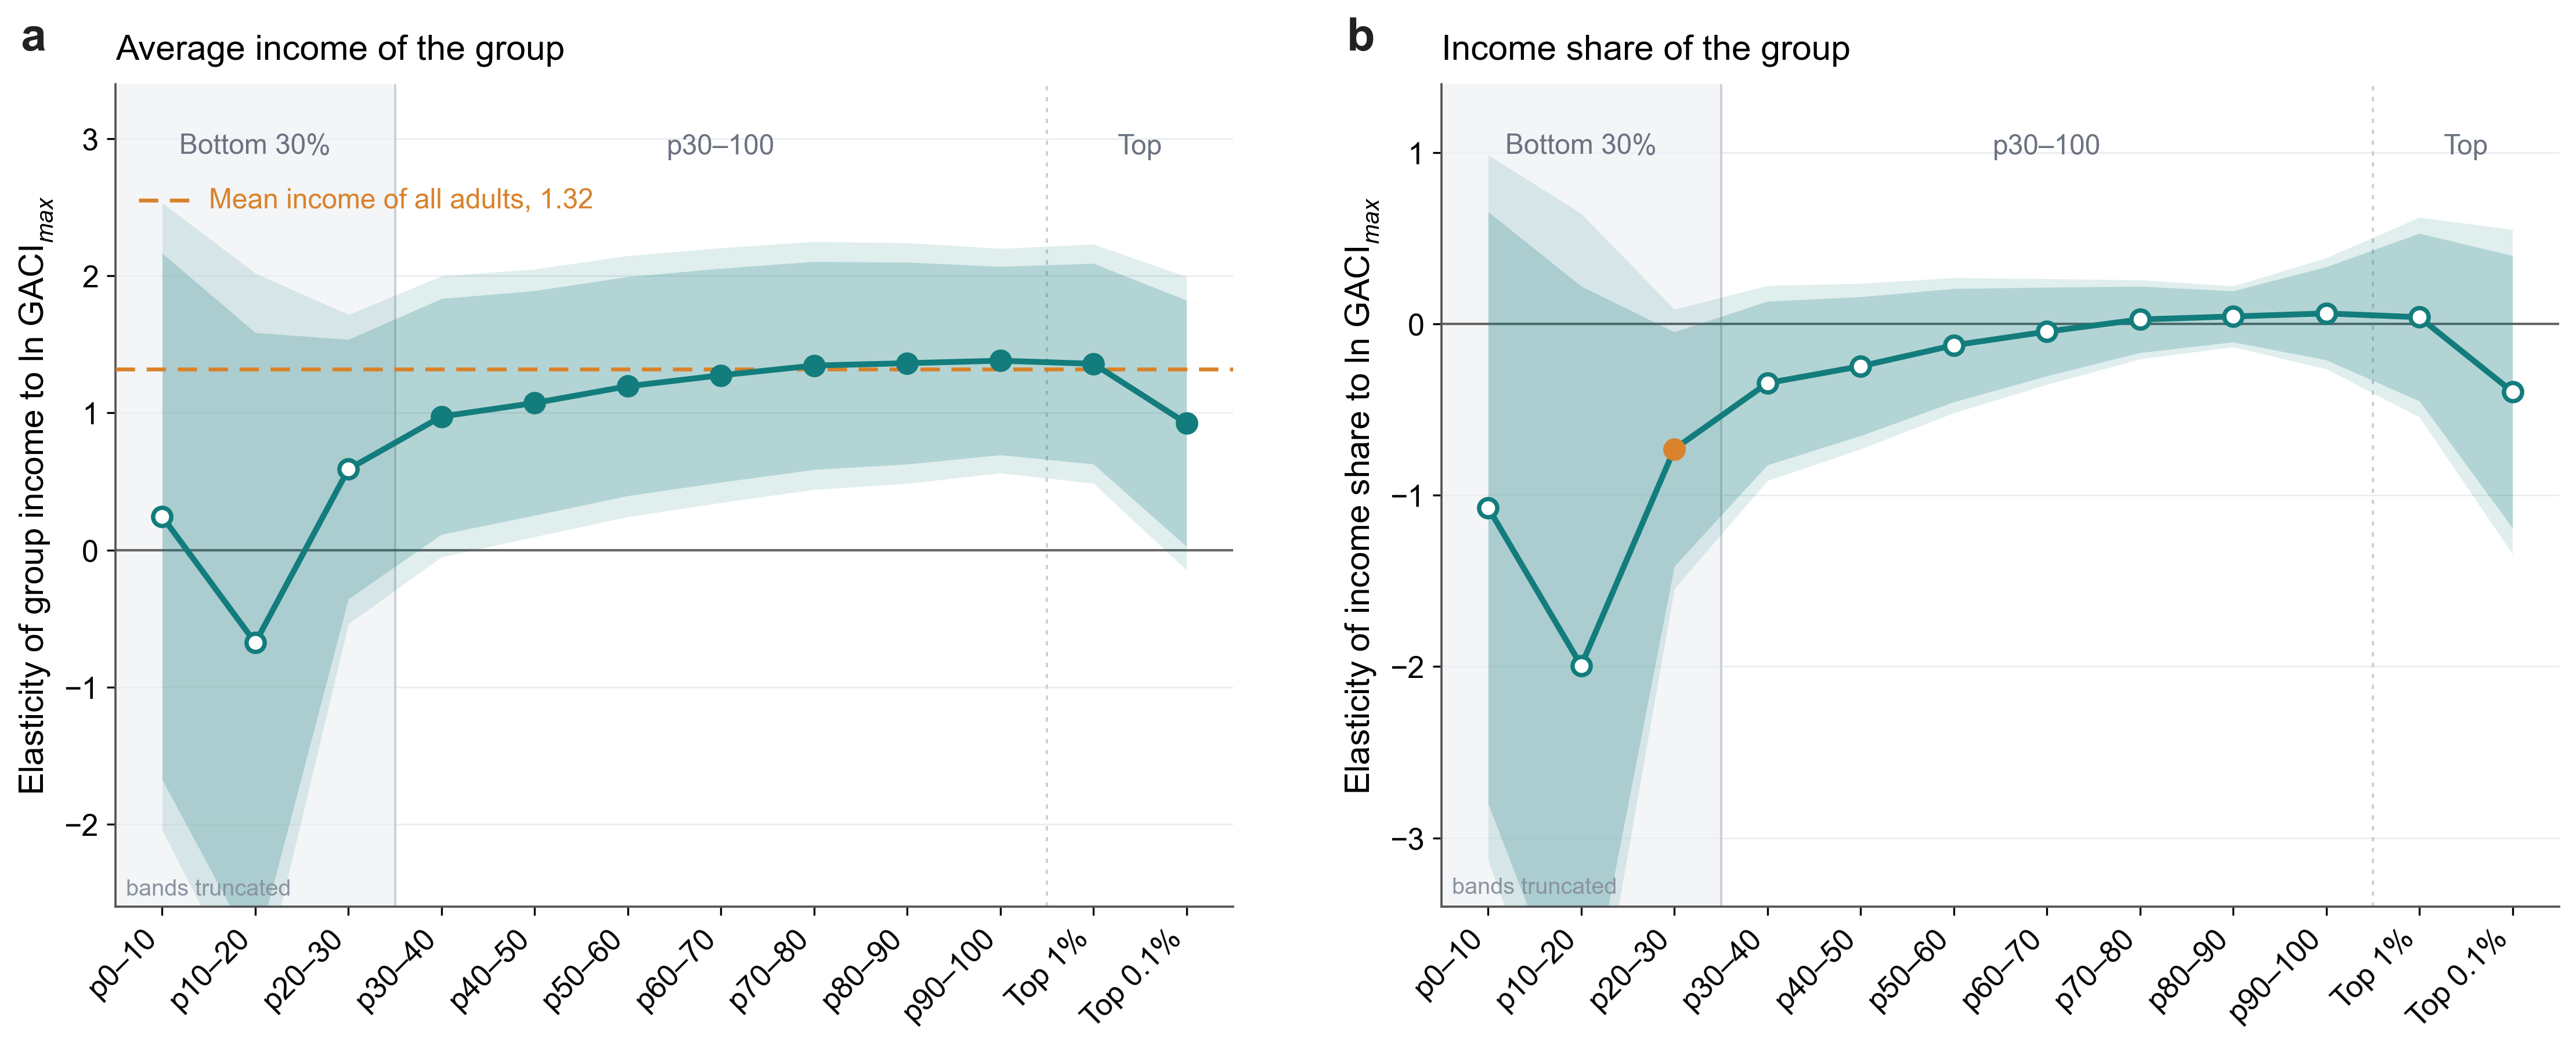
\includegraphics[width=\linewidth]{figures/FigW2_incidence.png}
\caption{Incidence of hub connectivity across the income distribution (2SLS, Feyrer instrument). (a) Elasticity of the average pretax income of each WID group to $\ln\mathrm{GACI}_{max}$; the dashed line is the elasticity of mean income of all adults. (b) Elasticity of the group's income share. The line connects the point estimates of Table~\ref{tab:incidence}; the dark and light bands are 90 and 95 percent confidence intervals clustered by country, truncated at the axis limits for the two lowest deciles. Filled markers denote $p<0.10$; amber markers denote significant negative estimates. The grey panel marks the bottom 30 percent of the distribution.}
\label{fig:incidence}
\end{figure}

The pattern is a step. Mean income of all adults rises with an elasticity of $1.32$ ($p<0.01$). From the fourth decile upward, group incomes rise with the mean: $0.97$ for p30--40 ($p<0.10$), $1.07$ for p40--50 ($p<0.05$), $1.20$ for p50--60 ($p<0.05$), and between $1.28$ and $1.38$ for the four deciles from p60--70 to p90--100 (all $p<0.01$). The top percentile rises by $1.36$ ($p<0.01$), the same as the top decile, and the difference between the two is $-0.02$ with a standard error of $0.19$. Because these groups rise at the rate of the mean, their shares do not change: every share elasticity from the fourth decile to the top percentile lies between $-0.35$ and $0.06$ and none is distinguishable from zero. Below the fourth decile the picture is different. The incomes of the three lowest deciles do not respond ($0.25$, $-0.68$ and $0.59$, none significant), and their shares fall: by $-1.07$ for the bottom decile (standard error $1.05$), $-2.00$ for the second ($1.35$) and $-0.73$ for the third ($p<0.10$). The share estimates for the two lowest deciles are imprecise, because their incomes are small and the least precisely measured part of the distribution, so the significant share loss is located at the third decile and in the aggregate: the bottom 30 percent has an income elasticity of $0.41$ (standard error $0.63$) and a share elasticity of $-0.91$ ($p<0.10$). Panel B reports the differences exactly: the top 30 percent's income rises by $0.95$ more than the bottom 30 percent's ($p<0.10$), whereas the differences between the top half and the bottom half ($0.45$), between the top decile and the bottom half ($0.48$) and between the top percentile and the top decile ($-0.02$) are not distinguishable from zero. The distribution divides at the third decile: above it no share moves, below it the shares fall, and no division appears anywhere else.

Two features of the step identify the mechanism. First, the growth that connectivity generates is not ordinary growth in the sense of \citet{Dollar_2016}: under their benchmark every decile would rise one-for-one with the mean, whereas here the three lowest deciles do not rise at all. Second, the top does not pull away from the rest. The top percentile and the top 0.1 percent do not gain relative to the top decile, and the shares of the top 10 and top 30 percent do not change. The response is broad across the upper seventy percent and absent at the bottom, the shape that sorting into the market economy of the connected place predicts, and not the concentration at the very top that skill-biased demand for the highest earners or innovation rents would produce \citep{Aghion_2018}. These results bear directly on \textbf{Hypothesis~2}, which predicts that the income arrives across the upper part of the distribution at the rate of the mean and does not arrive at the bottom, whose share falls, and that the top percentile does not gain relative to the top decile. \textbf{Hypothesis~2} is supported on all three counts.

%=======================================================================
\subsection{Growth and its incidence by baseline hub size}
\label{sec:growthstage}
The companion paper finds the largest income gains from connectivity in the least developed economies. We ask whether the bottom of the distribution is left out in the same economies, and whether growth and its incidence move together. Table~\ref{tab:growth_stage} splits countries on the connectivity of their hub in 1996 and reports, within each group, the 2SLS and OLS elasticities of GDP per capita, mean income, the income and share of the bottom 30 percent and the top-30-minus-bottom-30 gap, together with the first-stage statistic.

\begin{table}[p]
\centering
\caption{Growth and its incidence by baseline hub size (countries grouped on $\mathrm{GACI}_{max}$ in 1996).}
\label{tab:growth_stage}
\begin{minipage}{\linewidth}
\centering
\resizebox{\linewidth}{!}{%
\begin{tabular}{lcccccc}
\toprule
 & ln GDP p.c. & Mean income & Bottom-30\% income & Bottom-30\% share & Top-30 minus bottom-30 & KP $F$ / N \\
\midrule
\multicolumn{7}{l}{\emph{Panel A. Median split on $\mathrm{GACI}_{max}$ in 1996}}\\
Below median (smaller hubs): 2SLS & 1.748\sym{***} & 1.664\sym{***} & 1.403\sym{**} & -0.261 & 0.215 & 33.4 \\
 & (0.402) & (0.358) & (0.537) & (0.364) & (0.457) & N = 2{,}170 \\
\quad OLS & 0.855\sym{***} & 0.945\sym{***} & 0.931\sym{***} & -0.014 & 0.025 \\
 & (0.184) & (0.205) & (0.282) & (0.108) & (0.150) \\
Above median (larger hubs): 2SLS & 1.804 & 1.870 & -2.987 & -4.857 & 5.322 & 1.0 \\
 & (1.751) & (2.052) & (5.216) & (5.454) & (6.002) & N = 2{,}367 \\
\quad OLS & 0.821\sym{***} & 0.665\sym{***} & 0.641\sym{***} & -0.023 & 0.056 \\
 & (0.156) & (0.172) & (0.172) & (0.090) & (0.106) \\
\addlinespace\multicolumn{7}{l}{\emph{Panel B. Terciles}}\\
Low: 2SLS & 2.371\sym{***} & 2.123\sym{***} & 2.737\sym{***} & 0.614 & -0.882\sym{*} & 26.4 \\
 & (0.538) & (0.430) & (0.630) & (0.384) & (0.488) & N = 1{,}417 \\
\quad OLS & 1.206\sym{***} & 1.257\sym{***} & 1.475\sym{***} & 0.218 & -0.305\sym{*} \\
 & (0.121) & (0.119) & (0.188) & (0.135) & (0.174) \\
Middle: 2SLS & 1.176\sym{**} & 1.099\sym{*} & -0.449 & -1.548\sym{**} & 1.779\sym{**} & 9.4 \\
 & (0.574) & (0.628) & (0.851) & (0.623) & (0.718) & N = 1{,}513 \\
\quad OLS & 0.716\sym{***} & 0.611\sym{***} & 0.482\sym{*} & -0.129 & 0.201\sym{*} \\
 & (0.205) & (0.212) & (0.253) & (0.080) & (0.110) \\
High: 2SLS & -1.380 & -0.114 & -9.729 & -9.615 & 10.584 & 0.2 \\
 & (6.853) & (4.510) & (27.510) & (24.357) & (26.807) & N = 1{,}607 \\
\quad OLS & 0.735\sym{***} & 0.654\sym{***} & 0.608\sym{***} & -0.046 & 0.081 \\
 & (0.196) & (0.195) & (0.187) & (0.117) & (0.135) \\
\addlinespace\multicolumn{7}{l}{\emph{Reference}}\\
Full sample: 2SLS & 1.471\sym{***} & 1.320\sym{***} & 0.410 & -0.910\sym{*} & 0.951\sym{*} & 21.1 \\
 & (0.410) & (0.420) & (0.631) & (0.498) & (0.573) & N = 4{,}537 \\
\quad OLS & 0.810\sym{***} & 0.731\sym{***} & 0.728\sym{***} & -0.003 & 0.023 \\
 & (0.113) & (0.122) & (0.148) & (0.065) & (0.084) \\
\bottomrule
\end{tabular}}
\par\vspace{3pt}\begin{flushleft}\footnotesize Countries are grouped on their earliest observed $\mathrm{GACI}_{max}$ (1996 for most). GDP per capita from the World Development Indicators (constant 2015 US dollars). The instrument has no power among the largest hubs (upper half, top tercile), which are shown for completeness. Country-year panel of 178 economies, 1996--2023. All regressions include country and year fixed effects and log population. 2SLS instruments $\ln\mathrm{GACI}_{max}$ with the Feyrer interaction $Z_{ct}=a_t\times\ln\mathrm{MA}^{air}_{c,1996}$; KP $F$ is the Kleibergen--Paap $rk$ Wald statistic. Group incomes are the log average pretax national income of the group (WID, equal-split adults); shares are log income shares, computed as log group income minus log mean income so that all groups use the same sample. Standard errors clustered by country in parentheses. \sym{*}~$p<0.10$, \sym{**}~$p<0.05$, \sym{***}~$p<0.01$.\end{flushleft}
\end{minipage}
\end{table}


The first-stage column disciplines what can be read. The instrument has power among the smaller hubs, with $F$ of $33.4$ below the median and $26.4$ and $9.4$ in the low and middle terciles, and none among the larger hubs ($F$ of $1.0$ in the upper half and $0.2$ in the top tercile). This is a substantive fact rather than a nuisance: the global expansion of aviation moved the connectivity of hubs that were joining the network, not of the hubs that already anchored it, so the estimates describe hubs in their integrating phase. Within that phase the picture has two stages. Below the median, a one percent increase in hub connectivity raises GDP per capita by $1.75$ percent and mean income by $1.66$ percent ($p<0.01$), and the income of the bottom 30 percent rises by $1.40$ percent ($p<0.05$), so that its share does not fall ($-0.26$, standard error $0.36$). The terciles show that this average conceals a sequence. In the lowest tercile, where the hub is smallest, connectivity raises GDP per capita by $2.37$ percent and the income of the bottom 30 percent by $2.74$ percent (both $p<0.01$), more than mean income ($2.12$), so that the bottom's share rises ($0.61$) and the top-minus-bottom gap narrows ($-0.88$, $p<0.10$). In the middle tercile, where the hub is integrating from a moderate base, the growth response is smaller ($1.18$ for GDP per capita, $p<0.05$) and it bypasses the bottom: the income of the bottom 30 percent does not respond ($-0.45$), its share falls by $-1.55$ ($p<0.05$) and the gap widens by $1.78$ ($p<0.05$). Appendix Table~\ref{tab:a_stagedefs} shows the same sequence in quartiles and by baseline income. The sequence is the one the sorting mechanism implies: when a country first acquires international connectivity, the gain is broad and the bottom gains most; as the hub becomes a gateway, the gain concentrates in the part of the economy that the gateway connects to the world. These results bear on \textbf{Hypothesis~4}, which predicts that the bottom's loss is concentrated in hubs integrating from a moderate base, and support it.

%=======================================================================
\subsection{Mechanism: the hub, the channels, and the form of the network}
\label{sec:mechanism}
We now ask five questions about how hub connectivity leaves the bottom of the distribution out, each answered by a table. Together they describe a single chain: the pattern is carried by the hub rather than by the network (I); it takes the form of the upper seventy percent rising with the mean while the bottom thirty is bypassed (II); the exclusion is not transmitted by the growth channels that connectivity opens, each of which on its own raises the bottom's share, so that it is the direct effect of the hub net of the growth it generates (III); the bottom loses where connectivity is concentrated in one gateway and gains where it is dispersed, and the pattern does not cross borders (IV); and it is not offset by redistribution (V).

\paragraph{(I) Which connectivity carries the pattern?}
Table~\ref{tab:hub_network} separates the hub from the network for three outcomes: the bottom-30 share, the top-minus-bottom gap and mean income. Column (1) repeats the baseline. Column (2) adds total connectivity as a control: the coefficient on instrumented hub connectivity on the bottom-30 share moves from $-0.91$ to $-1.23$ ($p<0.10$), while total connectivity, which now measures the network net of the hub, enters at $+0.17$ ($p<0.10$). Holding the network fixed, the hub is the source of the bottom's loss and the rest of the network is, if anything, the source of its gain: a country whose connectivity grows through its secondary cities does not experience the exclusion that a country whose connectivity grows through its gateway does. Mean income, by contrast, responds to the hub alone ($1.34$ with the sum controlled, $p<0.05$) and not to the rest of the network ($-0.01$). Column (3) looks inside the hub. Instrumenting the hub's eigenvector centrality, its integration with the global core of the network, and controlling for its seat capacity gives $-0.35$ on centrality ($p<0.05$) and $+0.43$ on capacity ($p<0.10$) for the bottom-30 share, and the mirror image for the gap: it is the hub's integration with the world's core, not the volume of traffic it handles, that leaves the bottom out. These results bear on the first part of \textbf{Hypothesis~3}, that the pattern is specific to the hub, and support it.

\begin{table}[p]
\centering
\caption{Mechanism (I): which connectivity carries the effect?}
\label{tab:hub_network}
\begin{threeparttable}
\footnotesize
\begin{tabular}{lccc}
\toprule
 & (1) & (2) & (3) \\
 & Baseline & Hub + network & Core integration \\
\midrule
\multicolumn{4}{l}{\emph{Dependent variable: Bottom-30\% share}}\\
$\ln\mathrm{GACI}_{max}$ (hub), instrumented & -0.910\sym{*} & -1.228\sym{*} &  \\
 & (0.498) & (0.699) &  \\
$\ln\mathrm{GACI}_{sum}$ (whole network), control &  & 0.169\sym{*} &  \\
 &  & (0.100) &  \\
ln hub eigenvector centrality, instrumented &  &  & -0.345\sym{**} \\
 &  &  & (0.175) \\
ln hub seat capacity, control &  &  & 0.430\sym{*} \\
 &  &  & (0.220) \\
KP $F$ & 21.1 & 15.1 & 18.8 \\
Observations & 4{,}537 & 4{,}537 & 4{,}537 \\
\addlinespace
\multicolumn{4}{l}{\emph{Dependent variable: Top-30 minus bottom-30 income}}\\
$\ln\mathrm{GACI}_{max}$ (hub), instrumented & 0.951\sym{*} & 1.282 &  \\
 & (0.573) & (0.797) &  \\
$\ln\mathrm{GACI}_{sum}$ (whole network), control &  & -0.176 &  \\
 &  & (0.114) &  \\
ln hub eigenvector centrality, instrumented &  &  & 0.360\sym{*} \\
 &  &  & (0.201) \\
ln hub seat capacity, control &  &  & -0.449\sym{*} \\
 &  &  & (0.251) \\
KP $F$ & 21.1 & 15.1 & 18.8 \\
Observations & 4{,}537 & 4{,}537 & 4{,}537 \\
\addlinespace
\multicolumn{4}{l}{\emph{Dependent variable: Mean income}}\\
$\ln\mathrm{GACI}_{max}$ (hub), instrumented & 1.320\sym{***} & 1.343\sym{**} &  \\
 & (0.420) & (0.563) &  \\
$\ln\mathrm{GACI}_{sum}$ (whole network), control &  & -0.012 &  \\
 &  & (0.081) &  \\
ln hub eigenvector centrality, instrumented &  &  & 0.157 \\
 &  &  & (0.138) \\
ln hub seat capacity, control &  &  & -0.016 \\
 &  &  & (0.179) \\
KP $F$ & 21.1 & 15.1 & 18.8 \\
Observations & 4{,}537 & 4{,}537 & 4{,}537 \\
\addlinespace
\bottomrule
\end{tabular}
\begin{tablenotes}\small
\item Column (2) adds total connectivity as a control; column (3) instruments the hub's eigenvector centrality (integration with the global core) and controls for its seat capacity. Specification as in Table~\ref{tab:main}: country and year fixed effects, log population, $\ln\mathrm{GACI}_{max}$ instrumented by the Feyrer interaction; standard errors clustered by country in parentheses. \sym{*}~$p<0.10$, \sym{**}~$p<0.05$, \sym{***}~$p<0.01$.
\end{tablenotes}
\end{threeparttable}
\end{table}


\paragraph{(II) Who gains?}
Section~\ref{sec:incidence} answers this question, and Figure~\ref{fig:incidence} shows it: from the fourth decile to the top percentile every group rises at the rate of mean income, the three lowest deciles do not rise, and the distribution divides at the third decile.

\paragraph{(III) Is the exclusion carried by the growth channels?}
Connectivity raises GDP per capita with an elasticity of $1.47$, differentiated-goods trade by $2.33$, high value-to-weight trade by $2.09$, international tourist arrivals by $3.75$ and the industrial employment share by 16 points (Table~\ref{tab:channels}, column $a$; all $p<0.10$ or better), the channels that the aviation literature and the companion papers identify. Table~\ref{tab:channels} asks whether these induced changes transmit the bottom's loss, by decomposing the effect of hub connectivity on the bottom-30 share (Panel A), the bottom-30 income (Panel B) and mean income (Panel C) into the part that runs through each channel and the direct effect of the hub with the channel held fixed. The answer is that they do not transmit it; they work against it. Every channel, taken on its own, raises the bottom's share: the coefficient on GDP per capita in the share equation is $0.34$ ($p=0.06$), on differentiated and high value-to-weight trade $0.09$ and $0.08$ ($p<0.10$), on tourist arrivals $0.08$ and on industrial employment $0.010$ per point (both $p<0.01$). The transmitted part of the hub effect is therefore positive, between $0.17$ and $0.51$, and the direct effect of the hub, net of the growth it generates, is larger in magnitude than the total: $-1.42$ with GDP per capita held fixed against a total of $-0.91$, $-1.15$ and $-1.11$ with the two trade channels held fixed against $-0.94$, $-1.43$ with tourism against $-1.13$, and $-1.15$ with industrial employment against $-0.99$ (all $p<0.10$). Holding all five channels fixed at once gives a direct effect of $-2.25$ (standard error $1.21$) against a total of $-1.32$ on the 3{,}360 country-years with every channel observed. Panel B shows the same from the side of income: the bottom 30 percent's income does not respond to hub connectivity in total ($0.41$), but with GDP per capita held fixed the direct effect is $-1.46$ ($p<0.10$) and with all five channels fixed $-2.32$, so the growth that connectivity generates does reach the bottom and the hub takes back as much as it brings. Panel C confirms that the channels are the growth: GDP per capita absorbs the entire effect on mean income (direct $-0.04$), and each other channel absorbs between a fifth and two fifths of it. Because the channels are themselves outcomes of connectivity, the decomposition is an accounting under the assumption that the channel coefficients are not confounded, and it cannot rank the channels. What it establishes is the sign: if the bottom were excluded because tourism, high-value trade or industry did not employ it, holding those channels fixed would absorb the exclusion, whereas it enlarges it. The exclusion is the direct footprint of the hub, not a by-product of the growth it induces. This bears on the second part of \textbf{Hypothesis~3} and supports it.

\begin{table}[p]
\centering
\caption{Mechanism (III): is the exclusion of the bottom carried by the growth channels? Decomposition of the hub effect.}
\label{tab:channels}
\begin{minipage}{\linewidth}
\centering
\resizebox{\linewidth}{!}{%
\begin{tabular}{lccccccr}
\toprule
Channel $M$ & $a$: $\mathrm{GACI}_{max}\rightarrow M$ & $\theta$: $M\rightarrow$ outcome & Indirect $a\theta$ & Direct (hub) & Total & KP $F$ & N \\
\midrule
\multicolumn{8}{l}{\emph{Panel A. Bottom-30\% share}}\\
ln GDP per capita & 1.471\sym{***} (0.410) & 0.344\sym{*} (0.182) & 0.505 & -1.416\sym{*} (0.771) & -0.910\sym{*} (0.498) & 11.9 & 4{,}537 \\
ln differentiated-goods trade & 2.333\sym{***} (0.875) & 0.091\sym{*} (0.051) & 0.212 & -1.153\sym{*} (0.620) & -0.941\sym{*} (0.498) & 15.0 & 4{,}529 \\
ln high value-to-weight trade & 2.093\sym{**} (0.891) & 0.081\sym{*} (0.044) & 0.169 & -1.110\sym{*} (0.590) & -0.941\sym{*} (0.498) & 16.1 & 4{,}529 \\
ln international tourist arrivals & 3.749\sym{**} (1.478) & 0.082\sym{***} (0.031) & 0.306 & -1.434\sym{*} (0.757) & -1.128\sym{*} (0.641) & 15.5 & 3{,}516 \\
Employment in industry, \% & 15.96\sym{*} (8.38) & 0.010\sym{***} (0.004) & 0.166 & -1.153\sym{**} (0.564) & -0.987\sym{*} (0.526) & 16.7 & 4{,}317 \\
All five channels jointly & & & 0.927 & -2.245\sym{*} (1.214) & -1.319\sym{*} (0.711) & 8.4 & 3{,}360 \\
\addlinespace
\multicolumn{8}{l}{\emph{Panel B. Bottom-30\% income}}\\
ln GDP per capita & 1.471\sym{***} (0.410) & 1.272\sym{***} (0.192) & 1.870 & -1.461\sym{*} (0.800) & 0.410 (0.631) & 11.9 & 4{,}537 \\
ln differentiated-goods trade & 2.333\sym{***} (0.875) & 0.298\sym{***} (0.078) & 0.694 & -0.325 (0.762) & 0.370 (0.630) & 15.0 & 4{,}529 \\
ln high value-to-weight trade & 2.093\sym{**} (0.891) & 0.282\sym{***} (0.066) & 0.589 & -0.220 (0.715) & 0.370 (0.630) & 16.1 & 4{,}529 \\
ln international tourist arrivals & 3.749\sym{**} (1.478) & 0.162\sym{***} (0.038) & 0.606 & -0.252 (0.869) & 0.354 (0.778) & 15.5 & 3{,}516 \\
Employment in industry, \% & 15.96\sym{*} (8.38) & 0.024\sym{***} (0.007) & 0.389 & -0.211 (0.660) & 0.179 (0.654) & 16.7 & 4{,}317 \\
All five channels jointly & & & 2.316 & -2.316\sym{*} (1.262) & 0.000 (0.841) & 8.4 & 3{,}360 \\
\addlinespace
\multicolumn{8}{l}{\emph{Panel C. Mean income}}\\
ln GDP per capita & 1.471\sym{***} (0.410) & 0.928\sym{***} (0.061) & 1.365 & -0.045 (0.246) & 1.320\sym{***} (0.420) & 11.9 & 4{,}537 \\
ln differentiated-goods trade & 2.333\sym{***} (0.875) & 0.207\sym{***} (0.045) & 0.483 & 0.828\sym{*} (0.428) & 1.311\sym{***} (0.421) & 15.0 & 4{,}529 \\
ln high value-to-weight trade & 2.093\sym{**} (0.891) & 0.201\sym{***} (0.039) & 0.420 & 0.891\sym{**} (0.415) & 1.311\sym{***} (0.421) & 16.1 & 4{,}529 \\
ln international tourist arrivals & 3.749\sym{**} (1.478) & 0.080\sym{***} (0.026) & 0.300 & 1.182\sym{**} (0.494) & 1.482\sym{***} (0.478) & 15.5 & 3{,}516 \\
Employment in industry, \% & 15.96\sym{*} (8.38) & 0.014\sym{***} (0.005) & 0.223 & 0.942\sym{**} (0.406) & 1.165\sym{***} (0.422) & 16.7 & 4{,}317 \\
All five channels jointly & & & 1.389 & -0.071 (0.278) & 1.318\sym{***} (0.499) & 8.4 & 3{,}360 \\
\bottomrule
\end{tabular}}
\par\vspace{3pt}\begin{flushleft}\footnotesize Each row decomposes the 2SLS effect of $\ln\mathrm{GACI}_{max}$ on the outcome into the part transmitted by channel $M$ and the direct effect that remains with $M$ held fixed: Total $=$ Direct $+$ Indirect, where $a$ is the 2SLS effect of instrumented connectivity on $M$, $\theta$ is the coefficient on $M$ when it is added to the second stage, and the total is re-estimated on the channel's sample so that the identity holds exactly. The joint row holds all five channels fixed; its indirect column is the sum of the five indirect effects (total minus direct). Because the channels are themselves outcomes of connectivity, the decomposition is a Gelbach-type accounting under the assumption that the channel coefficient is not confounded, and is reported as descriptive. KP $F$ refers to the direct regression. Channels from the World Development Indicators and BACI. Country-year panel of 178 economies, 1996--2023. All regressions include country and year fixed effects and log population. 2SLS instruments $\ln\mathrm{GACI}_{max}$ with the Feyrer interaction $Z_{ct}=a_t\times\ln\mathrm{MA}^{air}_{c,1996}$; KP $F$ is the Kleibergen--Paap $rk$ Wald statistic. Group incomes are the log average pretax national income of the group (WID, equal-split adults); shares are log income shares, computed as log group income minus log mean income so that all groups use the same sample. Standard errors clustered by country in parentheses. \sym{*}~$p<0.10$, \sym{**}~$p<0.05$, \sym{***}~$p<0.01$.\end{flushleft}
\end{minipage}
\end{table}


\paragraph{(IV) Where is the pattern found?}
Table~\ref{tab:splits} and Figure~\ref{fig:where} split the sample along the dimensions the sorting mechanism singles out, and report for each subsample the first-stage statistic and the reduced-form $p$-value of the instrument for the bottom-30 share, which does not depend on first-stage strength. The form of the network is decisive. In economies whose connectivity was concentrated in one gateway in the base year (airport Gini above the median; the split uses the 161 economies with at least two airports), a rise in hub connectivity lowers the income of the bottom 30 percent ($-2.23$, $p<0.10$) and its share ($-2.17$, $p<0.05$; reduced-form $p=0.001$), widens the gap ($2.50$, $p<0.05$) and does not raise mean income ($-0.06$). In economies whose connectivity was dispersed across several airports, the same rise in hub connectivity raises mean income by $3.01$ percent and the income of the bottom 30 percent by $3.40$ percent (both $p<0.01$, with reduced-form $p$-values below 0.001 for the two income outcomes), so that the bottom's share does not fall ($0.39$) and the gap does not widen ($-0.64$). The first stage is above ten in both halves. Urbanisation gives the same contrast: above the median, the bottom-30 share falls ($-2.33$, $p<0.05$) and the gap widens; below it, mean income and the bottom's income rise by $2.5$ and $2.8$ percent ($p<0.01$) with no change in share. Baseline income repeats it in weaker form. The pattern is present in the 1996--2007 era, when the global expansion of aviation was fastest ($-1.48$ on the bottom-30 share, $p<0.01$), and not in 2010--2023, when the instrument moved connectivity less. Tourism dependence does not separate the economies: the bottom's share falls in both halves and neither is significant. The last two rows enter own connectivity together with the leave-out mean of contiguous neighbours' connectivity, each instrumented by its own shifter: the own effect on the bottom-30 share is $-1.49$ ($p<0.10$) and the neighbours' is $+0.64$ (standard error $0.55$); a neighbouring country's hub does not exclude the domestic bottom and, if anything, raises its income ($1.25$, $p<0.10$). The pattern is a property of the country's own gateway.

\begin{table}[H]
\centering
\caption{Mechanism (IV): where is the effect found? Split samples (2SLS, Feyrer instrument).}
\label{tab:splits}
\begin{minipage}{\linewidth}
\centering
\resizebox{\linewidth}{!}{%
\begin{tabular}{lcccccrr}
\toprule
 & Bottom-30\% share & Bottom-30\% income & Mean income & Top-30 minus bottom-30 & KP $F$ & RF $p$ & N \\
\midrule
Airport network concentrated (above median) & -2.174\sym{**} & -2.231\sym{*} & -0.057 & 2.504\sym{**} & 10.7 & 0.001 & 2{,}180 \\
 & (0.997) & (1.312) & (0.561) & (1.135) \\
Airport network dispersed (below median) & 0.388 & 3.402\sym{***} & 3.014\sym{***} & -0.644 & 10.3 & 0.450 & 2{,}018 \\
 & (0.519) & (1.042) & (0.842) & (0.642) \\
Urbanisation above median & -2.329\sym{**} & -1.423 & 0.906 & 2.603\sym{**} & 8.0 & 0.003 & 2{,}303 \\
 & (1.151) & (1.403) & (0.595) & (1.291) \\
Urbanisation below median & 0.243 & 2.750\sym{***} & 2.507\sym{***} & -0.432 & 11.7 & 0.670 & 2{,}234 \\
 & (0.567) & (0.905) & (0.703) & (0.679) \\
Baseline GDP per capita above median & -1.193\sym{*} & -0.548 & 0.646 & 1.359\sym{*} & 16.6 & 0.041 & 2{,}282 \\
 & (0.664) & (0.813) & (0.399) & (0.766) \\
Baseline GDP per capita below median & -0.709 & 2.562\sym{**} & 3.270\sym{***} & 0.533 & 5.4 & 0.372 & 2{,}255 \\
 & (0.915) & (1.173) & (1.155) & (1.035) \\
Tourism-dependent (above median) & -1.623 & 0.370 & 1.993\sym{**} & 1.600 & 7.2 & 0.090 & 2{,}099 \\
 & (1.281) & (1.301) & (0.763) & (1.428) \\
Not tourism-dependent (below median) & -0.369 & 0.337 & 0.706 & 0.452 & 12.1 & 0.349 & 2{,}181 \\
 & (0.377) & (0.648) & (0.507) & (0.444) \\
1996--2007 & -1.484\sym{***} & 0.466 & 1.950\sym{***} & 1.619\sym{**} & 19.2 & 0.003 & 1{,}860 \\
 & (0.557) & (0.654) & (0.488) & (0.630) \\
2010--2023 excluding 2020--21 & 0.123 & 1.026 & 0.903\sym{*} & -0.108 & 16.1 & 0.780 & 2{,}011 \\
 & (0.437) & (0.697) & (0.526) & (0.491) \\
\addlinespace
\multicolumn{8}{l}{\emph{Own and contiguous neighbours' connectivity, jointly instrumented (bottom-30\% share)}}\\
Own $\ln\mathrm{GACI}_{max}$ & -1.492\sym{*} & -0.724 & 0.768 & 1.735\sym{*} \\
 & (0.798) & (0.961) & (0.563) & (0.900) \\
Neighbours' ln GACI (contiguity, leave-out mean) & 0.639 & 1.246\sym{*} & 0.607 & -0.861 \\
 & (0.554) & (0.657) & (0.400) & (0.661) \\
\bottomrule
\end{tabular}}
\par\vspace{3pt}\begin{flushleft}\footnotesize Splits at the median of each country's earliest observed value: the Gini of GACI across its airports (network concentration), urbanisation, GDP per capita, and tourism receipts as a share of exports. RF $p$ is the $p$-value of the instrument in the reduced form for the bottom-30\% share, which does not depend on first-stage strength. The last two rows instrument own connectivity with the own shifter and the leave-out mean of contiguous neighbours' ln GACI with their shifters. Country-year panel of 178 economies, 1996--2023. All regressions include country and year fixed effects and log population. 2SLS instruments $\ln\mathrm{GACI}_{max}$ with the Feyrer interaction $Z_{ct}=a_t\times\ln\mathrm{MA}^{air}_{c,1996}$; KP $F$ is the Kleibergen--Paap $rk$ Wald statistic. Group incomes are the log average pretax national income of the group (WID, equal-split adults); shares are log income shares, computed as log group income minus log mean income so that all groups use the same sample. Standard errors clustered by country in parentheses. \sym{*}~$p<0.10$, \sym{**}~$p<0.05$, \sym{***}~$p<0.01$.\end{flushleft}
\end{minipage}
\end{table}


\begin{figure}[H]
\centering
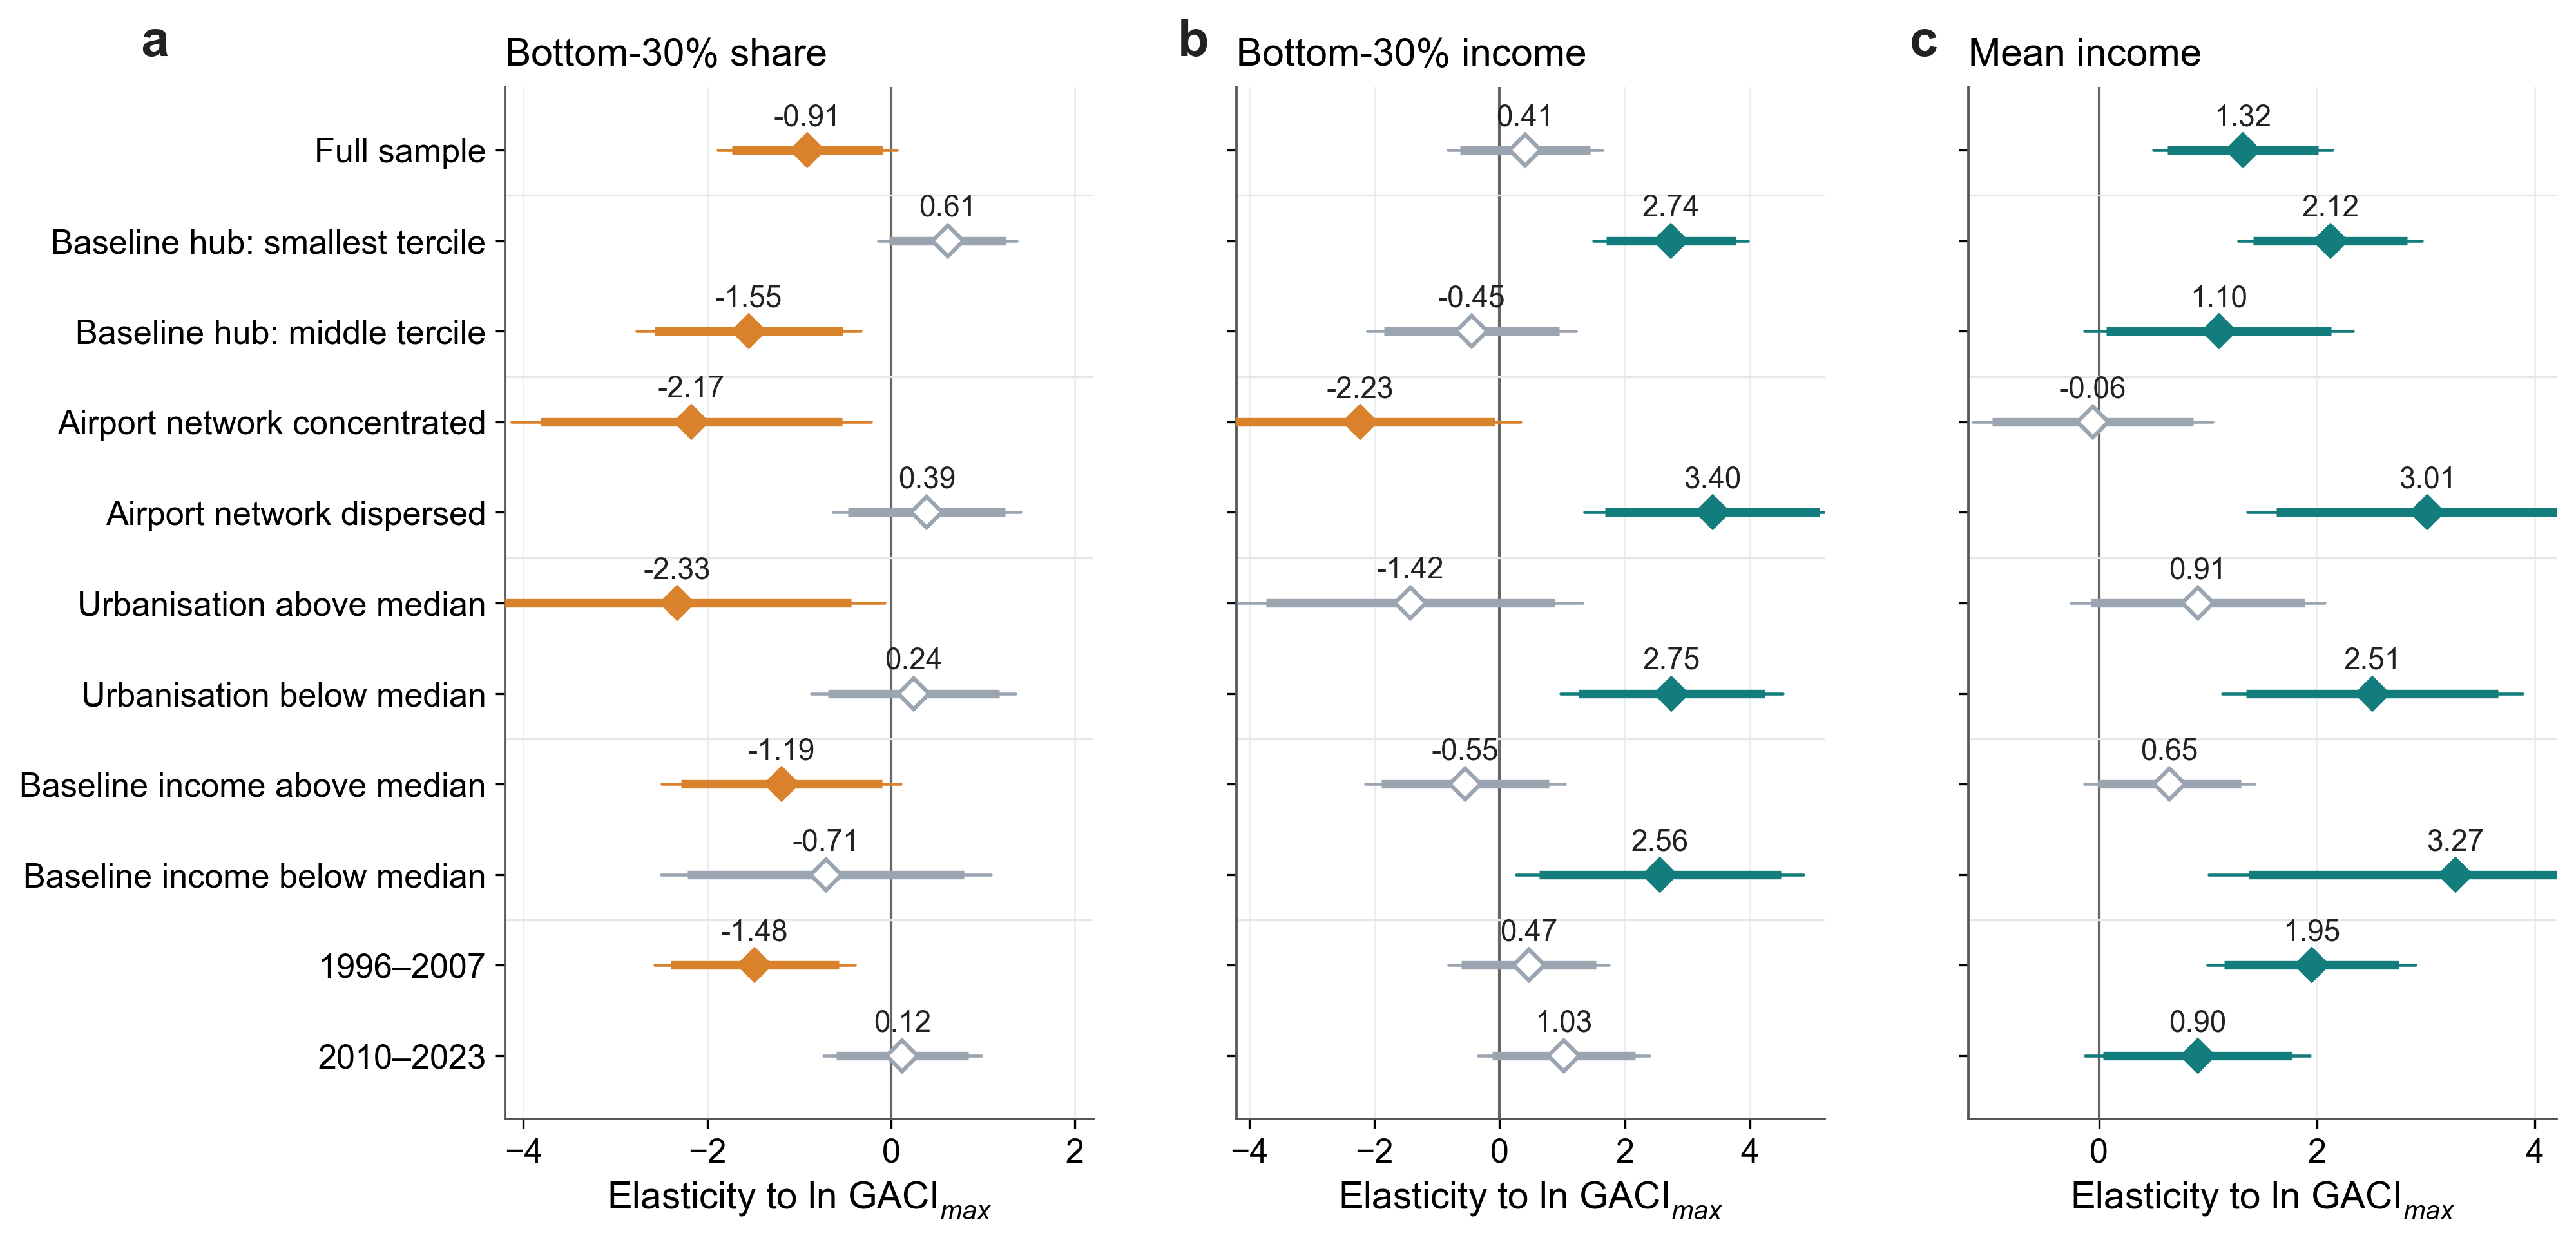
\includegraphics[width=\linewidth]{figures/FigW3_where.png}
\caption{Where the income arrives: split-sample 2SLS elasticities to $\ln\mathrm{GACI}_{max}$. (a) Bottom-30\% share. (b) Bottom-30\% income. (c) Mean income. Rows are the full sample, terciles of baseline hub size, and median splits on the concentration of the airport network, urbanisation and baseline income, and the two eras. Diamonds are point estimates; thick bars are 90 percent and thin bars 95 percent confidence intervals clustered by country; filled markers denote $p<0.10$, teal for positive and amber for negative estimates. First-stage statistics and reduced-form $p$-values are in Tables~\ref{tab:growth_stage} and \ref{tab:splits}.}
\label{fig:where}
\end{figure}

\paragraph{(V) Is the pattern offset by redistribution?}
Finally, Table~\ref{tab:redistribution} asks whether taxes and transfers offset the market outcome, using the WID's post-tax national income shares. They do not. The pretax share of the bottom half falls by $-0.42$ (standard error $0.31$) and its post-tax share by $-0.63$ ($p<0.05$); the difference, the redistribution the bottom half receives, falls by $-0.21$ (reduced-form $p=0.07$). The top decile's pretax share does not change ($0.06$) while its post-tax share rises by $0.18$, and the difference rises by $0.12$ ($p<0.05$). Taxes and transfers in the economies whose hubs integrated did not expand toward the bottom to meet its exclusion from market growth; they moved, if anything, in the other direction, which is the pattern the evidence on globalisation and the tax burden would predict \citep{Egger_2019,Kleven_2013}. This completes the test of \textbf{Hypothesis~4}: the bottom loses where connectivity is concentrated and gains where it is dispersed, the loss is concentrated in urbanised economies and in hubs integrating from a moderate base, it does not cross borders, and it is not offset by redistribution.

\begin{table}[H]
\centering
\caption{Mechanism (V): is the effect offset by redistribution? Pretax and post-tax income shares (WID).}
\label{tab:redistribution}
\begin{threeparttable}
\small
\begin{tabular}{lcccc}
\toprule
 & \multicolumn{2}{c}{OLS} & \multicolumn{2}{c}{2SLS} \\
\cmidrule(lr){2-3}\cmidrule(lr){4-5}
 & Coef. & (s.e.) & Coef. & (s.e.) \\
\midrule
Bottom-50\% share, pretax & -0.037 & (0.053) & -0.419 & (0.309) \\
Bottom-50\% share, post-tax & -0.059 & (0.048) & -0.629\sym{**} & (0.318) \\
Post-tax minus pretax, bottom 50\% & -0.022 & (0.020) & -0.210 & (0.127) \\
Top-10\% share, pretax & 0.046 & (0.037) & 0.061 & (0.165) \\
Top-10\% share, post-tax & 0.049 & (0.038) & 0.181 & (0.186) \\
Post-tax minus pretax, top 10\% & 0.003 & (0.010) & 0.120\sym{**} & (0.058) \\
\midrule
KP $F$ & & & \multicolumn{2}{c}{21.1} \\
Observations & \multicolumn{2}{c}{4{,}537} & \multicolumn{2}{c}{4{,}537} \\
\bottomrule
\end{tabular}
\begin{tablenotes}\small
\item Post-tax national income shares from the WID distributional national accounts (after all taxes and transfers). The difference rows are difference outcomes: a negative coefficient for the bottom 50\% means that taxes and transfers redistribute less toward the bottom half after connectivity rises. Country-year panel of 178 economies, 1996--2023. All regressions include country and year fixed effects and log population. 2SLS instruments $\ln\mathrm{GACI}_{max}$ with the Feyrer interaction $Z_{ct}=a_t\times\ln\mathrm{MA}^{air}_{c,1996}$; KP $F$ is the Kleibergen--Paap $rk$ Wald statistic. Group incomes are the log average pretax national income of the group (WID, equal-split adults); shares are log income shares, computed as log group income minus log mean income so that all groups use the same sample. Standard errors clustered by country in parentheses. \sym{*}~$p<0.10$, \sym{**}~$p<0.05$, \sym{***}~$p<0.01$.
\end{tablenotes}
\end{threeparttable}
\end{table}


%=======================================================================
\subsection{Robustness}
\label{sec:robust}
Table~\ref{tab:robust} probes the headline estimates along four dimensions and replaces the bottom-30 share by other summaries of the distribution. Panel B varies the sample: excluding the ten largest hub economies gives $-0.97$ on the bottom-30 share and $1.43$ on mean income ($p<0.10$ and $p<0.01$), restricting the sample to 1996--2019 gives $-0.76$ and $1.25$, and excluding the financial-crisis and pandemic years gives $-0.71$ and $1.34$; the mean-income estimate is significant at 1 percent in every sample, and the bottom-30 share estimate keeps its sign and magnitude, with $p$-values of 0.11 and 0.12 in the two restricted samples. Panel C addresses the exclusion restriction with the controls of Section~\ref{sec:strategy}, each a competing exposure interacted with the same shifter. The interactions of baseline GDP per capita and of land area with the shifter leave the estimates unchanged ($-0.91$ and $-0.85$ on the bottom-30 share, $1.49$ and $1.36$ on mean income, first stages of $21.5$ and $22.5$). The maritime control is more demanding, because air and sea market access are computed from the same population geography and are highly collinear across countries: with $\mathrm{MA}^{sea}_{c,1996}\times a_t$ in the equation the first stage falls to $6.5$, the mean-income elasticity rises to $2.56$ ($p<0.05$) and the bottom-30 share estimate keeps its sign and size, $-0.86$, with a standard error that doubles to $0.80$. The point estimates therefore do not move when the maritime channel is partialled out; what the control removes is precision, since little of the air-specific variation remains once sea access is held fixed. Panel D varies the variance estimator; the Conley rows are re-estimated on the 4{,}334 country-years of the 165 economies with centroid coordinates, so their point estimates differ slightly from the baseline. Two-way clustering by country and year and Conley spatial HAC with 1{,}000 and 2{,}000 km cutoffs \citep{Conley_1999} leave the mean-income estimate significant at 5 percent or better and place the bottom-30 share estimate at the margin of conventional significance ($p$ between 0.10 and 0.14), so the share result should be read as an estimate whose sign is stable and whose precision is limited by the slow movement of the distribution. Panel E replaces the bottom-30 share by other summaries of the same distribution. The bottom-50 share, the Palma ratio, the WID Gini and the top-10 share all move in the direction of the headline and none is significant, which is what the step at the third decile implies: summaries that weight the middle and the top, which do not move, cannot detect a change confined to the bottom three deciles. The absolute gap between the top decile and the bottom half, the one summary that responds to the level of income, rises with an elasticity of $1.40$ ($p<0.01$). Appendix Table~\ref{tab:a_swiid} reports the subsample of 166 economies for which survey-based Gini coefficients are available: there, the market and disposable Gini rise with elasticities of $0.50$ and $0.66$ ($p<0.05$ and $p<0.01$), the bottom-30 share falls by $-1.48$ ($p<0.10$) and the bottom-50 share by $-0.77$ ($p<0.10$), so the survey-based measures agree with the WID incidence.

\begin{table}[p]
\centering
\caption{Robustness of the headline estimates: sample, exclusion restriction, inference and alternative measures (2SLS, Feyrer instrument).}
\label{tab:robust}
\begin{minipage}{\linewidth}
\centering
\resizebox{\linewidth}{!}{%
\begin{tabular}{lcccrr}
\toprule
 & Bottom-30\% share & Top-30 minus bottom-30 & Mean income & KP $F$ & N \\
\midrule
\multicolumn{5}{l}{\emph{Panel A. Baseline}}\\
2SLS, Feyrer instrument (Table~\ref{tab:main}) & -0.910\sym{*} (0.498) & 0.951\sym{*} (0.573) & 1.320\sym{***} (0.420) & 21.1 & 4{,}537 \\
\multicolumn{5}{l}{\emph{Panel B. Sample}}\\
Excluding the ten largest hub economies & -0.968\sym{*} (0.524) & 1.020\sym{*} (0.602) & 1.425\sym{***} (0.447) & 19.0 & 4{,}262 \\
1996--2019 & -0.764 (0.479) & 0.795 (0.556) & 1.251\sym{***} (0.401) & 21.8 & 3{,}864 \\
Excluding 2008--09 and 2020--21 & -0.705 (0.457) & 0.735 (0.531) & 1.343\sym{***} (0.412) & 22.7 & 3{,}871 \\
\multicolumn{5}{l}{\emph{Panel C. Exclusion restriction: competing exposure $\times$ shifter as control}}\\
$\ln\mathrm{MA}^{sea}_{c,1996}\times a_t$ (maritime market access) & -0.857 (0.797) & 0.777 (0.929) & 2.561\sym{**} (1.115) & 6.5 & 4{,}537 \\
Baseline ln GDP per capita $\times a_t$ & -0.913\sym{*} (0.514) & 0.949 (0.591) & 1.492\sym{***} (0.364) & 21.5 & 4{,}537 \\
ln land area $\times a_t$ & -0.855\sym{*} (0.466) & 0.884 (0.538) & 1.364\sym{***} (0.418) & 22.5 & 4{,}537 \\
\multicolumn{5}{l}{\emph{Panel D. Inference}}\\
Clustered by country & -0.910\sym{*} (0.498) & 0.951\sym{*} (0.573) & 1.320\sym{***} (0.420) & 21.1 & 4{,}537 \\
Two-way clustered (country, year) & -0.910 (0.538) & 0.951 (0.610) & 1.320\sym{***} (0.420) &  & 4{,}537 \\
Conley spatial HAC, 1{,}000 km & -0.821 (0.508) & 0.849 (0.584) & 1.218\sym{**} (0.511) &  & 4{,}334 \\
Conley spatial HAC, 2{,}000 km & -0.821 (0.557) & 0.849 (0.647) & 1.218\sym{**} (0.619) &  & 4{,}334 \\
\multicolumn{6}{l}{\emph{Panel E. Alternative distributional measures, 2SLS (coefficient in the first column)}}\\
Bottom-50\% share & -0.419 (0.309) & & & & 4{,}537 \\
Palma ratio (top 10 / bottom 40) & 0.621 (0.512) & & & & 4{,}537 \\
WID Gini & 0.060 (0.134) & & & & 4{,}537 \\
Top-10\% share & 0.061 (0.165) & & & & 4{,}537 \\
Absolute gap, top 10 minus bottom 50 & 1.402\sym{***} (0.425) & & & & 4{,}537 \\
\bottomrule
\end{tabular}}
\par\vspace{3pt}\begin{flushleft}\footnotesize Panel C adds, one at a time, a competing baseline exposure interacted with the aviation shifter $a_t$ (Section~\ref{sec:strategy}); $\mathrm{MA}^{sea}$ is Equation~\eqref{eq:ma} computed with CERDI port-to-port sea distances. Panel D varies the variance estimator. The two-way clustered row keeps the baseline point estimates; the Conley rows are re-estimated on the 4{,}334 country-years of the 165 economies with centroid coordinates, so their point estimates differ slightly. Conley standard errors use a Bartlett kernel in great-circle distance between country centroids and allow arbitrary within-country serial correlation. Panel E replaces the bottom-30\% share by other summaries of the same WID distribution: Palma $=$ top-10 share / bottom-40 share; the absolute gap is the top-10 minus bottom-50 average income in constant local prices; the WID Gini is the DINA Gini. Specification as in Table~\ref{tab:main}: country and year fixed effects, log population, $\ln\mathrm{GACI}_{max}$ instrumented by the Feyrer interaction; standard errors clustered by country in parentheses. \sym{*}~$p<0.10$, \sym{**}~$p<0.05$, \sym{***}~$p<0.01$.\end{flushleft}
\end{minipage}
\end{table}


%=======================================================================
\subsection{Aggregate contribution of connectivity growth, 1996--2023}
\label{sec:aggregate}
How much of the change in the distribution over the sample period do the estimates attribute to hub connectivity? For each of the 162 countries with at least fifteen years of data, we multiply the observed change in $\ln\mathrm{GACI}_{max}$ between the first and last year by the 2SLS elasticities of Table~\ref{tab:main}: for mean income and for the income of the top and bottom 30 percent in percent, and for the bottom-30 share converted to points of national income using each country's initial share. Figure~\ref{fig:attribution} ranks the countries with the largest implied changes in the bottom-30 share and maps the implied share change and the implied growth of mean income; Appendix Table~\ref{tab:a_aggregate} reports regional and world aggregates against the observed changes.

\begin{figure}[H]
\centering
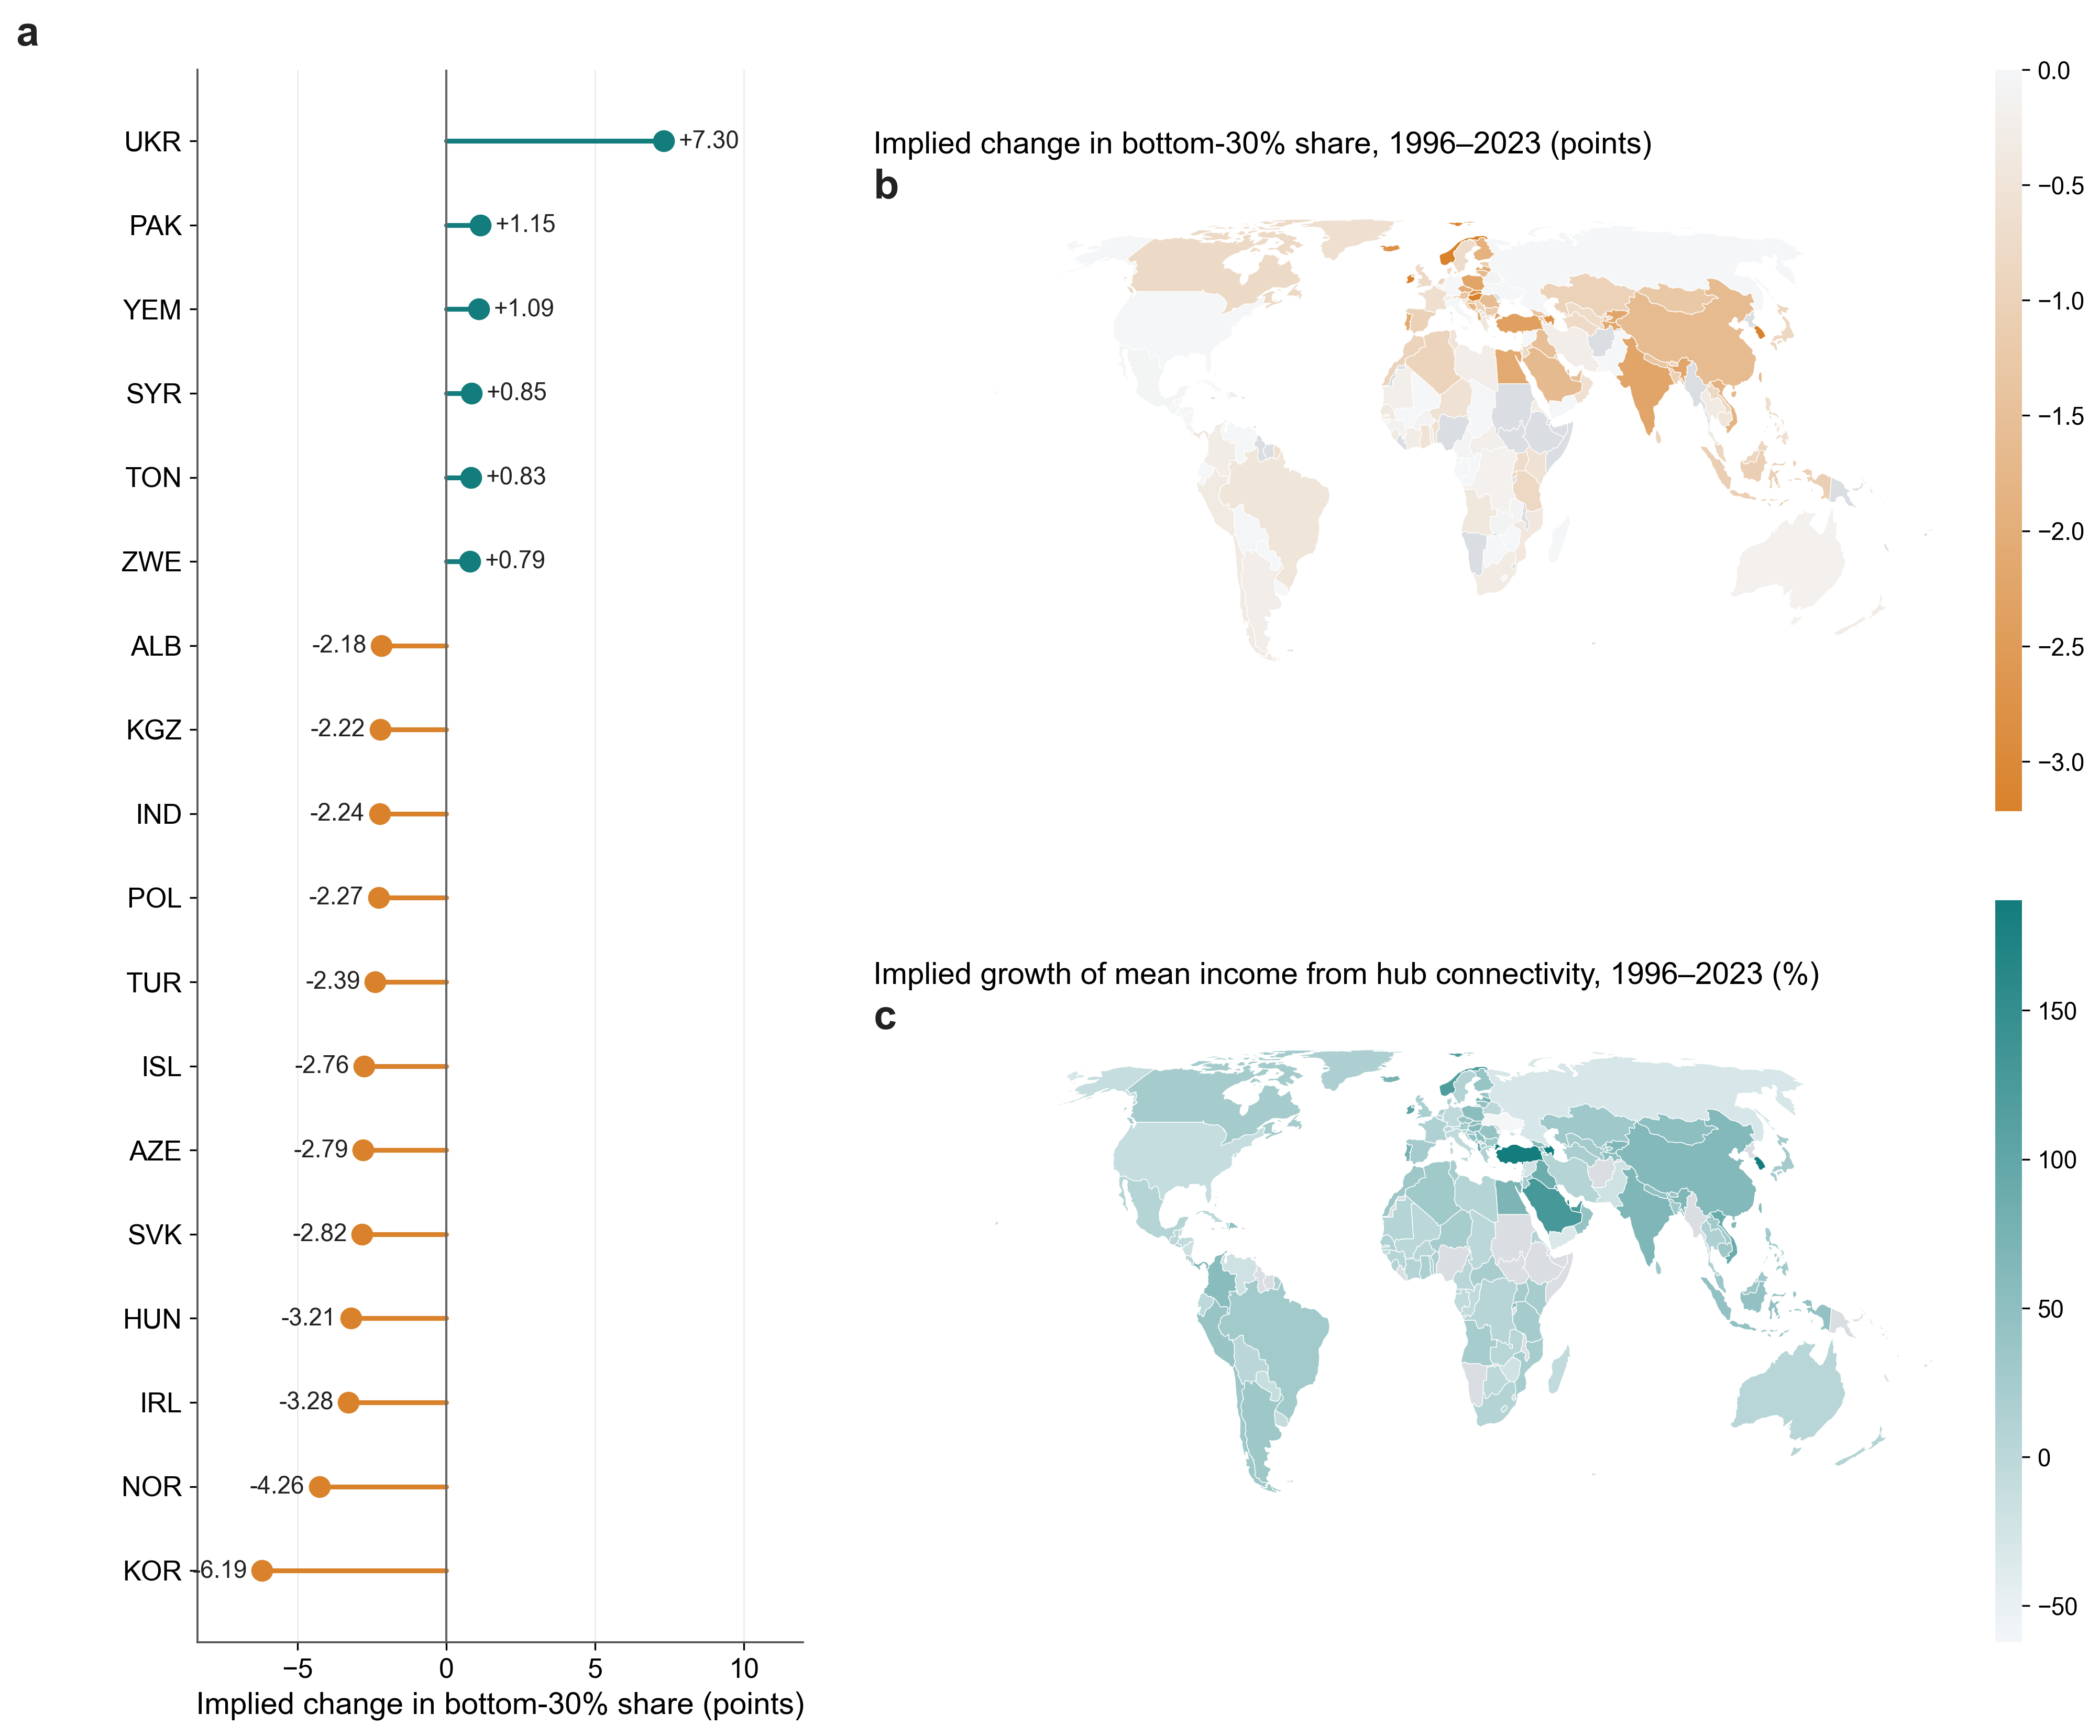
\includegraphics[width=\linewidth]{figures/FigW4_attribution.png}
\caption{Implied incidence of observed hub-connectivity growth, 1996--2023. (a) Countries with the largest implied decreases and increases in the bottom-30\% share of pretax national income, in points, from the observed change in $\ln\mathrm{GACI}_{max}$ multiplied by the 2SLS elasticity of Table~\ref{tab:main}. (b) Implied change in the bottom-30\% share by country. (c) Implied growth of mean income by country, in percent. Grey denotes countries with fewer than fifteen years of data.}
\label{fig:attribution}
\end{figure}

Hub connectivity rose in 81 percent of the 162 countries, by $0.15$ log points on average and by $0.23$ when countries are weighted by population. Applied to the elasticities, this growth implies an increase of 27 percent in mean income for the unweighted average country and of 41 percent for the population-weighted world, against observed increases of 65 and 139 percent; connectivity growth accounts for about three tenths of world income growth over the period on this accounting. For the top 30 percent the implied increase is the same as for the mean, 29 and 43 percent; for the bottom 30 percent it is 7 and 10 percent. The implied change in the bottom-30 share is $-0.7$ points of national income for the average country and $-1.05$ points for the population-weighted world, against observed changes of $+0.1$ and $-0.7$ points. The largest implied losses are in the economies whose hubs became global gateways over the period, Korea ($-6.2$ points, from a one-log-point increase in hub connectivity), Norway ($-4.3$), Ireland ($-3.3$), Hungary and Slovakia ($-3.2$ and $-2.8$), Turkey ($-2.4$) and India ($-2.2$); the implied changes are positive where hub connectivity fell, as in Ukraine, Pakistan and Yemen. By region, the implied loss is largest in Asia-Pacific and Europe ($-1.2$ points each) and smallest in Latin America and Africa ($-0.1$ and $-0.3$), where hubs grew less. The comparison says two things. First, hub-connectivity growth was a large part of income growth over the period, and almost all of that part accrued to the upper seventy percent. Second, in the population-weighted world the bottom-30 share fell by about what connectivity growth alone would imply, while in the average country other forces raised it slightly; the exclusion of the bottom from connectivity-driven growth is, on this accounting, one of the larger forces acting on the bottom of national distributions over the period. As in the companion paper, this is a partial-equilibrium accounting that holds elasticities constant and abstracts from adjustment in prices, migration and policy; it is a statement of the order of magnitude the estimates imply, not a decomposition of history.

%=======================================================================
\subsection{Synthesis: the hypotheses revisited}
\label{sec:synthesis}
The results map onto the four hypotheses of Section~\ref{sec:framework} as follows. \textbf{Hypothesis~1}, that hub connectivity increases mean income, is supported: the elasticity is $1.32$, it holds across the three aggregations of connectivity and in every sample and inference variant (Tables~\ref{tab:main} and \ref{tab:robust}). \textbf{Hypothesis~2}, that the income arrives across the upper part of the distribution at the rate of the mean and not at the bottom, whose share falls, and that the top percentile does not pull away, is supported: from the fourth decile to the top percentile every group rises with the mean and no share changes, the three lowest deciles do not rise and their shares fall, and the top percentile moves with the top decile (Table~\ref{tab:incidence}). \textbf{Hypothesis~3}, that the pattern is specific to the hub and is not transmitted by the growth channels connectivity opens, is supported: with the network held fixed the hub lowers the bottom's share and the rest of the network raises it, integration with the global core carries the pattern within the hub, and the increases in GDP per capita, differentiated and high value-to-weight trade, tourism and industrial employment that connectivity induces each raise the bottom's share, so that the direct effect of the hub, net of the growth it generates, is larger than the total (Tables~\ref{tab:hub_network} and \ref{tab:channels}). \textbf{Hypothesis~4}, that the bottom loses where connectivity is concentrated and gains where it is dispersed, that the loss is concentrated in urbanised economies and integrating hubs, does not spill across borders and is not offset by redistribution, is supported (Tables~\ref{tab:growth_stage}, \ref{tab:splits} and \ref{tab:redistribution}).

Read jointly, the four verdicts tell one story rather than four. Hub connectivity raises national income, and the income arrives at the part of the distribution that participates in the market economy the gateway connects to the world, the upper seventy percent, at the rate of the mean. It does not arrive at the bottom thirty percent, whose share falls. The exclusion is not transmitted by the growth that connectivity generates, since holding that growth fixed enlarges rather than absorbs it; it is not a property of connectivity in general, since a dispersed network includes the bottom; and it is not a top-percentile phenomenon, since the very top does not pull away. It is the footprint of a gateway on the distribution of the country that possesses it, largest at the moment the gateway is forming, and it is not offset by the tax and transfer system. Taken together, these results carry three messages. First, the national income gain from hub connectivity is real and large, and its incidence is broad but not universal: the average return overstates the return to the bottom thirty percent, which does not participate. Second, the exclusion is a consequence of the form connectivity growth takes, concentration in a single gateway, rather than of connectivity as such; the same connectivity distributed across several airports reaches the bottom first. Third, redistribution did not follow the hub, so the distributional outcome of hub development is a policy choice that governments made by default.

%=======================================================================
\section{Discussion}
\label{sec:discussion}
%=======================================================================
The central finding of this study is that the connectivity of a country's primary hub raises national income and that the income arrives across the distribution from the fourth decile upward and not below it. The 2SLS estimate for mean income implies an elasticity of $1.32$, and the incidence estimates show that this is the average of an elasticity of about $1.0$ to $1.4$ for the upper seventy percent of the distribution and an elasticity indistinguishable from zero for the bottom thirty percent, whose share of national income falls. This is a more precise statement than a summary index conveys. A change in the Gini could arise from many shapes of incidence, and the summaries of the distribution that weight the middle and the top, which do not move, register no change at all; the decile estimates show that the shape is a step with its riser at the third decile, that the top percentile moves with the rest of the top decile, and that the change is confined to the bottom. The result therefore does not describe a superstar economy, nor one in which the middle class is squeezed. It describes an economy in which the broad segment that participates in the market economy connected to the world, from the lower-middle class upward, receives the return to the country's connectivity at the same rate, while the bottom three deciles grow at the rate they would have grown without it.

The mechanism analysis helps explain why this shape arises and where the evidence is stronger and weaker. Three findings support a sorting-and-agglomeration interpretation over the alternatives. First, the hub, not the network, carries the pattern: with total connectivity held fixed, hub connectivity remains the source of the bottom's loss and the rest of the network is the source of its gain, and within the hub the evidence, which is suggestive because a single instrument cannot separate the components, points to integration with the global core rather than volume. A dispersed network connects secondary cities to the world and spreads the connectivity-related activity across places; a gateway concentrates it. Second, the exclusion is not transmitted by the growth that connectivity generates. Connectivity raises GDP per capita, differentiated and high value-to-weight exports, tourism and industrial employment, and each of these induced changes, taken on its own, raises the bottom's share of income: the growth channels are equalising. The exclusion is what remains when they are held fixed, the direct effect of the hub, and it is larger than the total effect because the growth partly offsets it. If the bottom were excluded because tourism or high-value trade did not employ it, holding those channels fixed would absorb the effect; instead it enlarges it, which indicates that the bottom is excluded by the concentration of connectivity-related activity in the hub rather than by the nature of the activity the hub generates. Third, the form of the network decides who gains. In economies whose connectivity was concentrated in a single gateway, the bottom thirty percent loses income and share when the hub grows; in economies whose connectivity was dispersed across several airports, the bottom thirty percent gains more than the mean. The decomposition should be interpreted as descriptive rather than as causal mediation, because each channel is itself an outcome of connectivity and its coefficient is identified only if it is not confounded, but the sign is the same for every channel and it is the sign the sorting mechanism predicts.

The redistribution result deserves emphasis because it is the margin on which policy operates. The post-tax share of the bottom half falls by more than its pretax share, and the post-tax share of the top decile rises while its pretax share does not. Governments in the economies whose hubs integrated did not expand redistribution toward the bottom to meet its exclusion from market growth. One reading is the one the globalisation literature suggests: the gains accrue to mobile high earners and firms, the tax burden has shifted toward the middle, and the political economy of a gateway city favours investment in the gateway over transfers away from it \citep{Egger_2019,Kleven_2013}. Whatever the reason, the finding means that the distributional outcome of hub development is not an unavoidable consequence of connectivity; it is the joint outcome of a concentrated form of connectivity growth and a tax and transfer system that did not respond to it.

The heterogeneity results reconcile this paper with the companion finding that connectivity raises income most in the least developed economies. The two findings are not in tension; they are two moments of one process. When a country whose hub is small acquires international connectivity, the gain is large and it reaches the bottom of the distribution first: in the lowest tercile of baseline hub size the income of the bottom thirty percent rises faster than the mean. As the hub grows into a gateway, the gain persists but concentrates in the part of the economy the gateway serves, and the bottom is left out. The instrument identifies precisely these two phases, since the global expansion of aviation moved the connectivity of hubs that were integrating and not of the hubs that already anchored the network; the estimates are therefore most informative about hubs in the integrating phase and about connectivity changes of the kind the aviation cycle induces, and they say little about the marginal effect of connectivity at London, Frankfurt or Tokyo. A country deciding whether to develop a gateway is, however, in exactly the phase the estimates describe.

The aggregate accounting puts the magnitudes in perspective. Applied to observed connectivity growth, the elasticities imply that hub integration raised mean income in the population-weighted world by two fifths over 1996--2023, about three tenths of observed growth, and that almost all of the gain accrued to the upper seventy percent: the implied gain for the bottom thirty percent is one quarter of the implied gain for the top thirty, and the implied loss of one point of national income in the bottom-30 share matches the loss actually observed in the population-weighted world. The accounting is partial-equilibrium and holds elasticities constant, so it indicates orders of magnitude; but the order of magnitude is that hub development was one of the larger forces acting on the bottom of national distributions over the period, in both directions: it raised the bottom's income where connectivity was dispersed and left it out where connectivity was concentrated.

The policy implications follow. Airport and route investment and air-service liberalisation raise national income, and this paper does not qualify that conclusion. It qualifies its incidence. Where connectivity growth takes the form of a single gateway, the return accrues to the upper seventy percent of the distribution and the tax system, on the evidence here, does not redistribute it. Two policy margins follow from the mechanism. The first is the form of the network: because dispersed connectivity reaches the bottom of the distribution, the development of secondary international airports and of direct international service from second-tier cities is a way to obtain the income gain and include the bottom in it, and the positive coefficient on network connectivity net of the hub indicates that it may raise the bottom's share. The second is redistribution: the exclusion is concentrated in an identifiable phase of hub development and in identifiable economies, so a government that develops a gateway can anticipate it and respond with transfers, with investment in the connectivity of other regions, or with the spatial policies whose trade-offs \citet{Fajgelbaum_2020} analyse. The argument against doing nothing is that the default, on this evidence, is growth that the bottom three deciles do not share.

The study has limitations. First, the instrument identifies the effect of connectivity changes induced by the global aviation cycle in hubs that were integrating into the network; it has no power in the largest hubs and the estimates should not be extrapolated to them. Second, the channel decomposition is descriptive, as discussed above. Third, the WID decile series combine survey, tax and national-accounts data whose quality varies across countries, and the incomes of the lowest deciles are the least precisely measured; the estimates for the bottom two deciles are correspondingly imprecise, and the bottom-30 share estimate is at the margin of conventional significance under spatial and two-way clustering. The agreement between the WID incidence and the survey-based Gini coefficients on the subsample where both exist is reassuring but does not remove measurement error. Fourth, the aggregate accounting is partial equilibrium. Fifth, the split-sample estimates have weaker first stages than the pooled sample, which is why we report reduced-form $p$-values alongside them. Extending the design to sub-national income data, so that the hub region and the rest of the country can be observed separately, and embedding the elasticities in a spatial equilibrium model in which migration, housing and wages adjust, are the natural next steps.

%=======================================================================
\section{Conclusion}
\label{sec:conclusion}
%=======================================================================
The evidence in this paper indicates that the connectivity of a country's primary hub raises national income and that the income does not reach the bottom of the distribution. Instrumenting a continuous, network-based connectivity index with a Feyrer-type interaction between the global aviation cycle and baseline geographic air market access, we estimate an elasticity of mean income of $1.32$ for 178 economies over 1996--2023, robust to the sample, to spatial and two-way clustered inference and to the aggregation of connectivity. Decile-level estimates show where the income arrives: every group from the fourth decile to the top percentile rises at the rate of the mean, so that no share above the third decile changes, while the three lowest deciles do not rise and their share of national income falls. The pattern is carried by the hub and not by the national network, by integration with the global core and not by traffic volume, and it is not transmitted by the growth that connectivity opens, in income, trade, tourism or industrial employment, each of which on its own includes the bottom; it is the direct effect of the hub net of that growth. Where the growth arrives depends on the form of the network: in economies whose connectivity is concentrated in one gateway the bottom thirty percent loses, and in economies whose connectivity is dispersed across several airports it gains the most. Taxes and transfers do not offset the market outcome. Nearly three decades of hub-connectivity growth account for about three tenths of world income growth and for a loss of one point of national income in the bottom-30 share of the population-weighted world. Hub development raises average income and leaves the bottom of the distribution out in the same movement; the income gain from connectivity is real, and so is its incidence. The policy implication is that the form connectivity growth takes, and the redistribution that accompanies it, determine whether a country's gateway is a national asset or an asset of the part of the country that the gateway serves.

%=======================================================================
\appendix
%=======================================================================
\section{Additional figures and tables}
\label{sec:appendix}
Figure~\ref{fig:evolution} describes the evolution of the global air network over the sample period and Figure~\ref{fig:mapchange} maps the change in hub connectivity that identifies the estimates. Table~\ref{tab:a_stagedefs} reports the growth-and-incidence split under alternative baseline groupings, Table~\ref{tab:a_swiid} the subsample with survey-based Gini coefficients, and Table~\ref{tab:a_aggregate} the regional and world aggregates underlying Figure~\ref{fig:attribution}.

\begin{figure}[H]
\centering
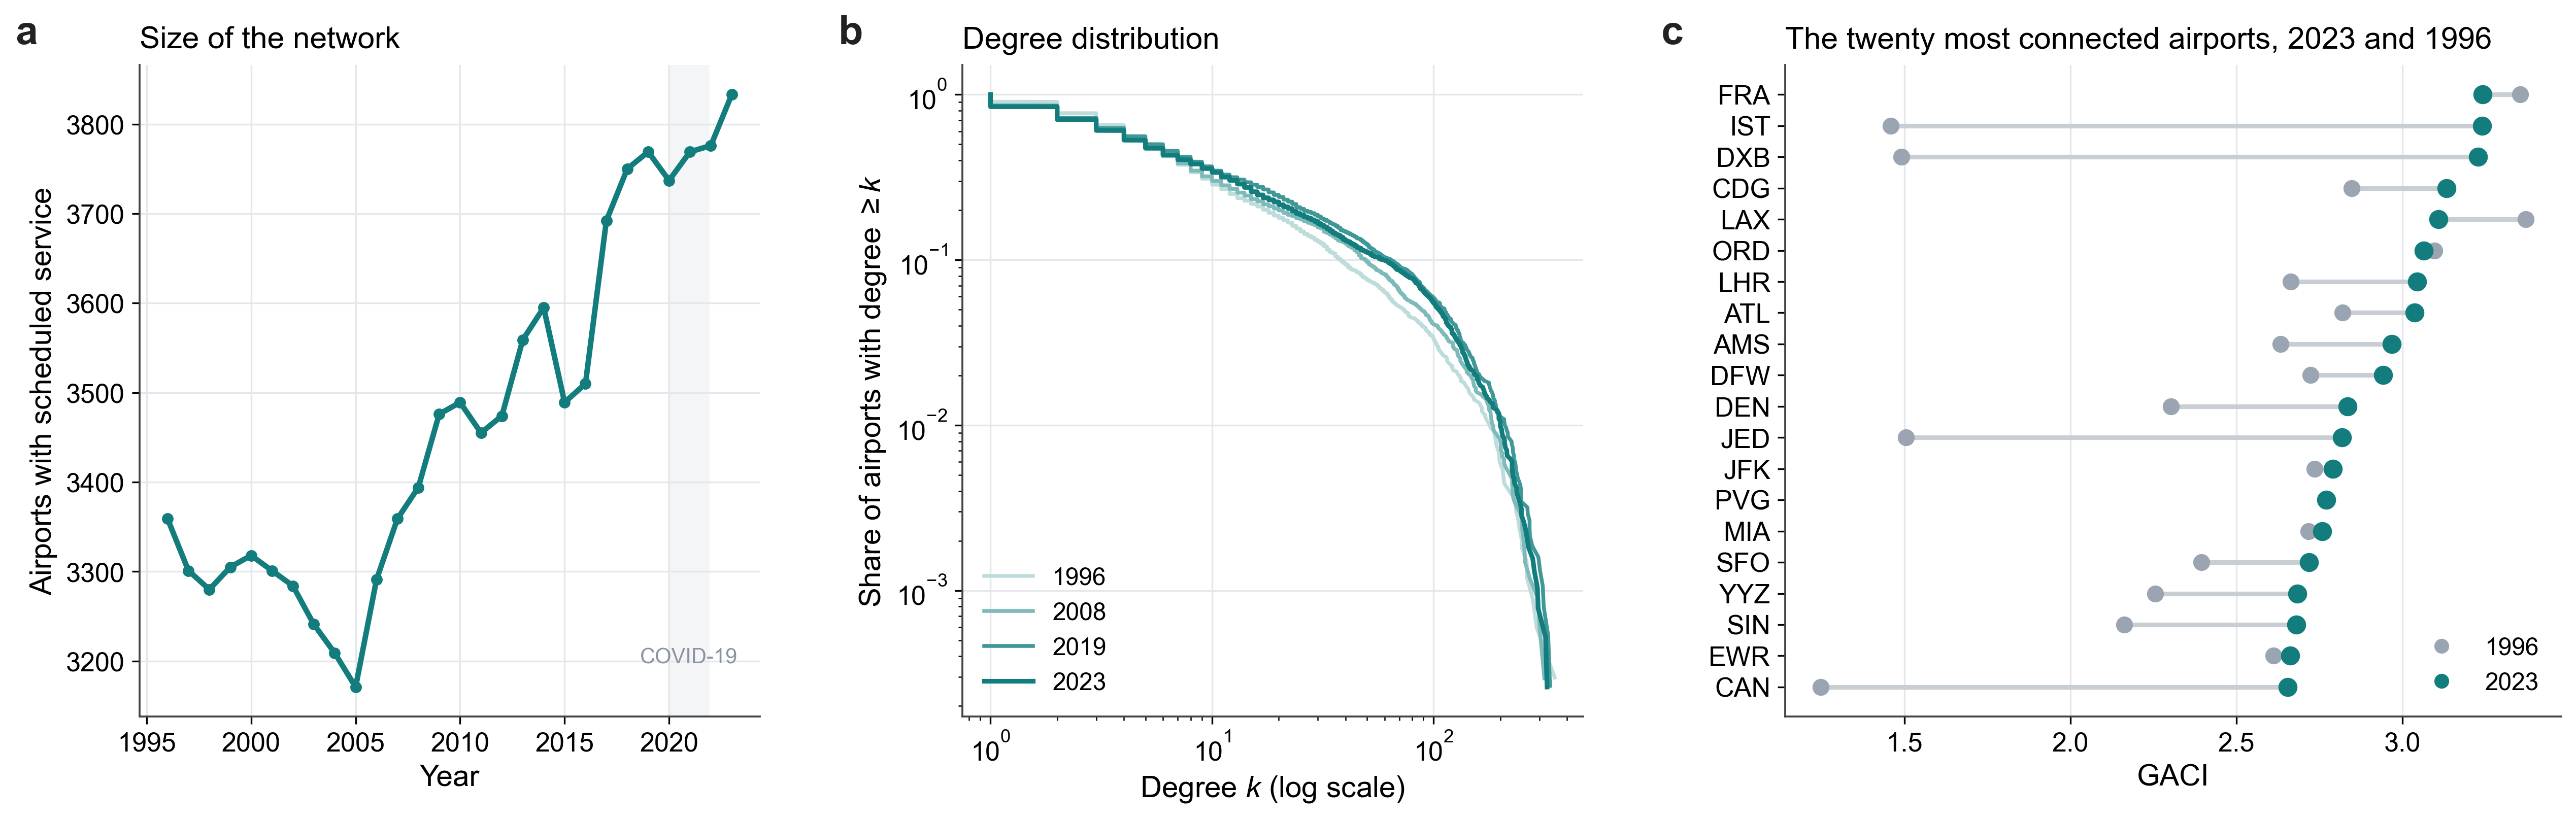
\includegraphics[width=\linewidth]{figures/FigB2_network_evolution.png}
\caption{Evolution of the global air network, 1996--2023. (a) Number of airports with scheduled service in each year's network. (b) Complementary cumulative distribution of degree (share of airports with at least $k$ direct connections) in 1996, 2008, 2019 and 2023, log scales. (c) The twenty airports with the highest GACI in 2023 (teal) and their index in 1996 (grey). Source: authors' airport-year panel.}
\label{fig:evolution}
\end{figure}

\begin{figure}[H]
\centering
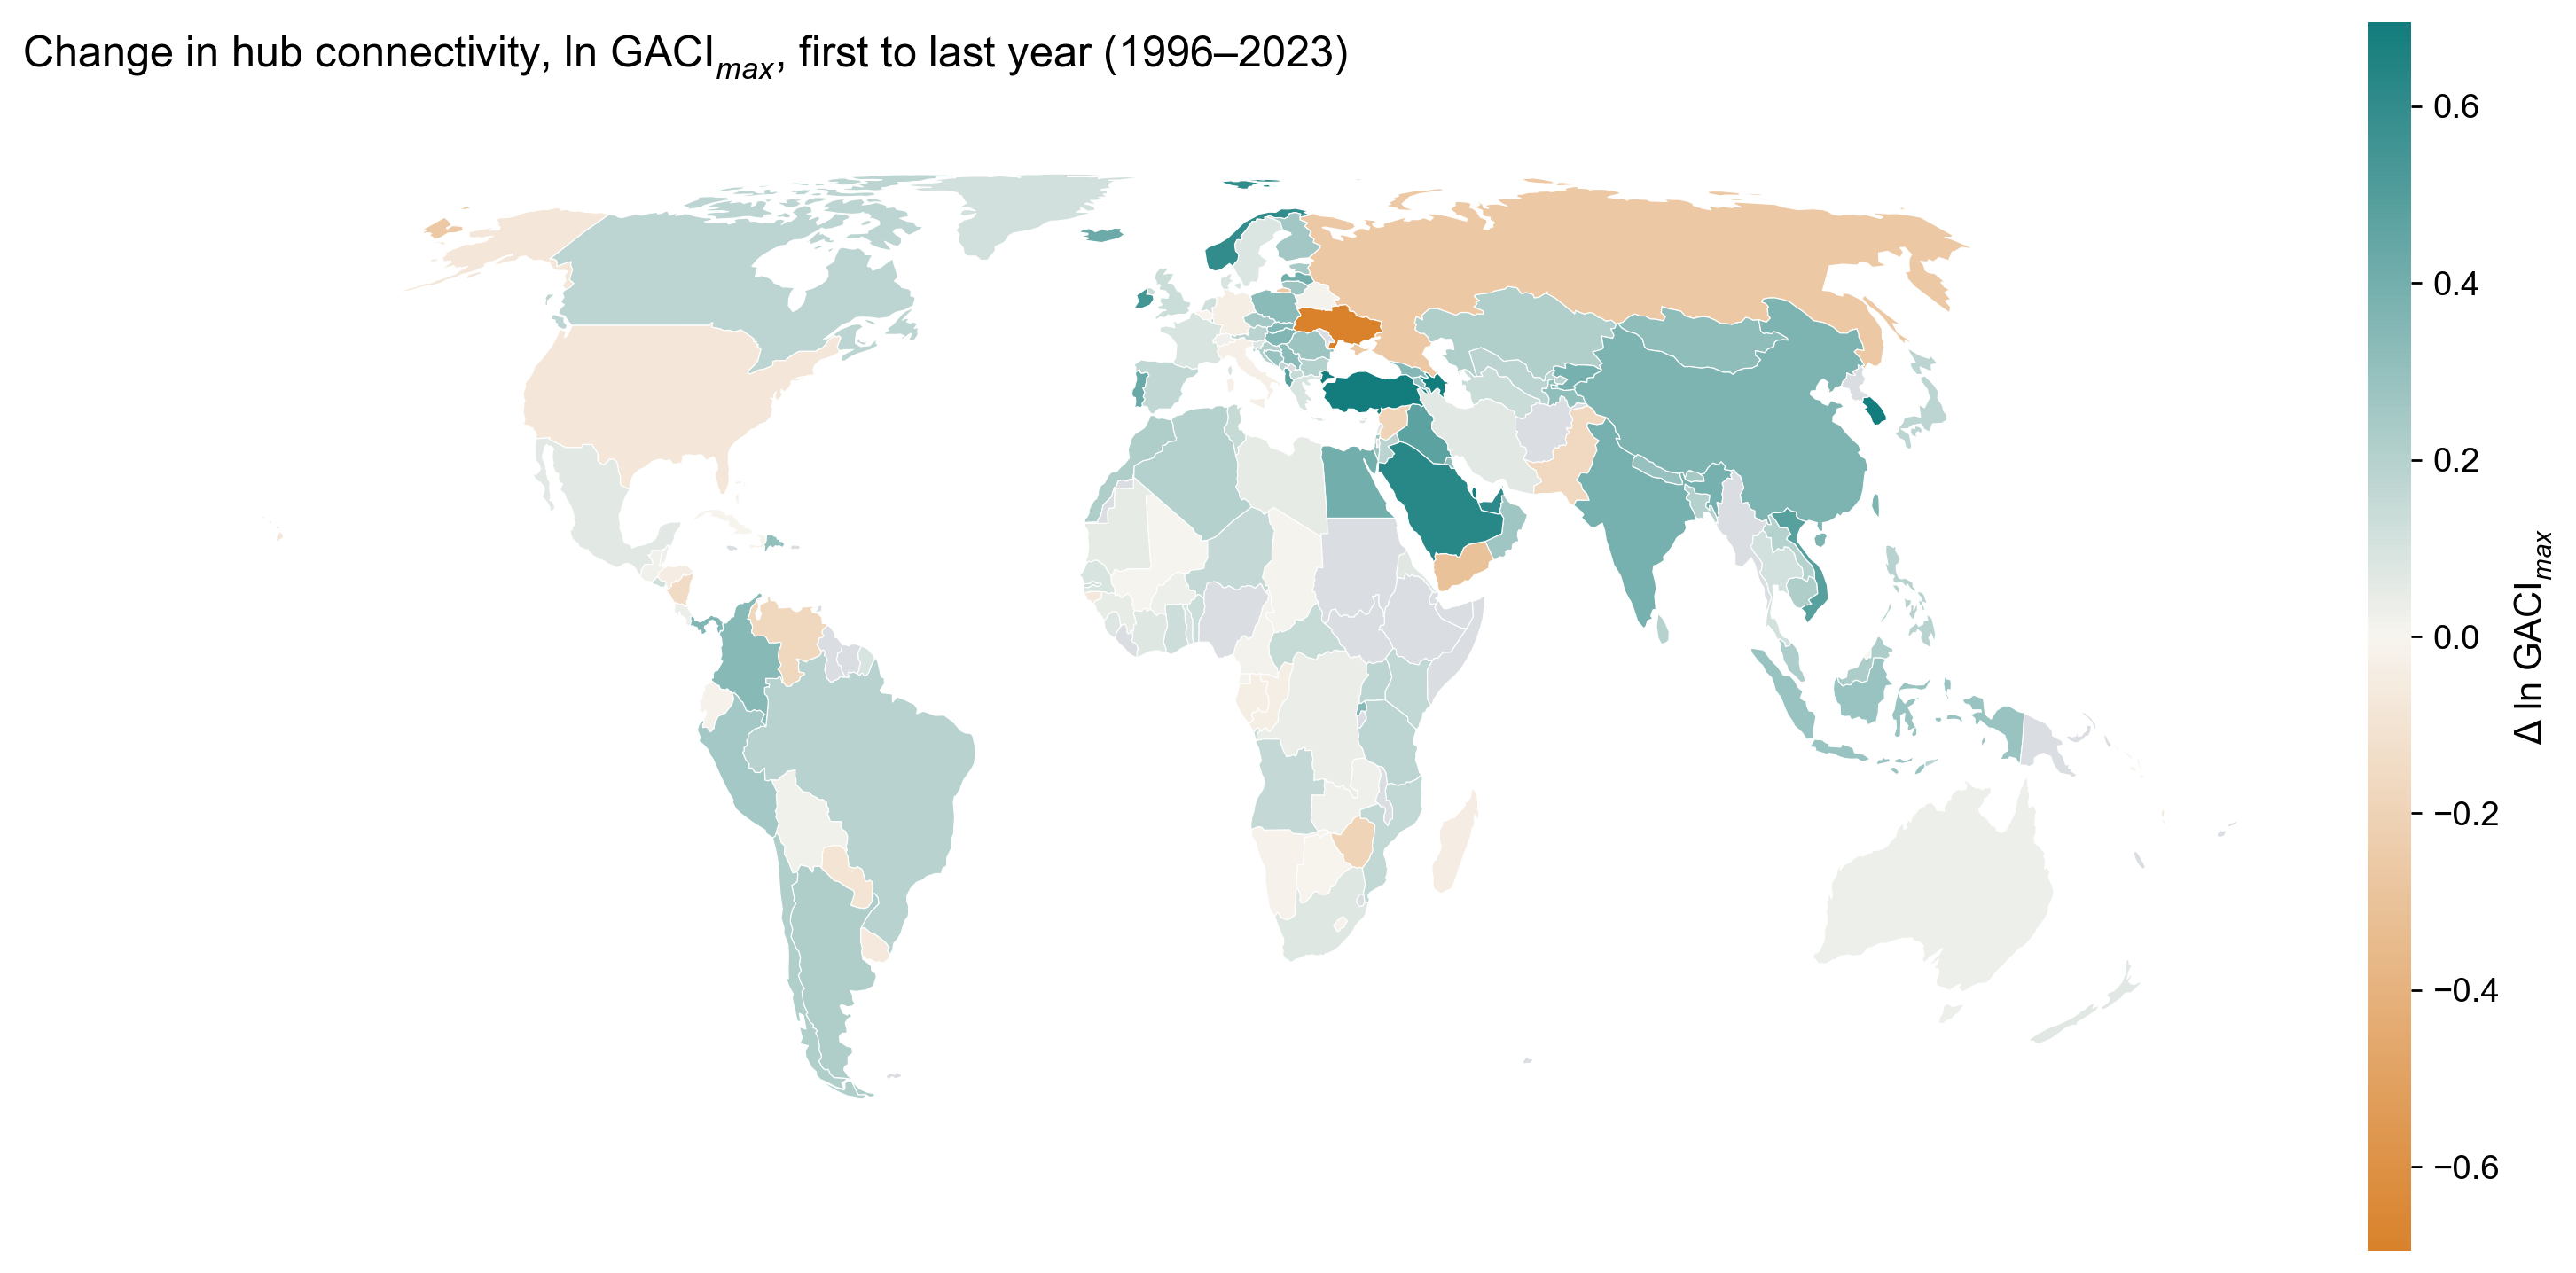
\includegraphics[width=\linewidth]{figures/FigB4_map_change.png}
\caption{Change in hub connectivity by country, $\ln\mathrm{GACI}_{max}$, between each country's first and last year in the panel (at least fifteen years apart). Teal denotes increases and amber decreases; grey denotes countries with fewer than fifteen years of data. Equal Earth projection.}
\label{fig:mapchange}
\end{figure}

\begin{table}[H]
\centering
\caption{Growth and its incidence under alternative baseline groupings (2SLS).}
\label{tab:a_stagedefs}
\begin{minipage}{\linewidth}
\centering
\resizebox{\linewidth}{!}{%
\begin{tabular}{lcccccc}
\toprule
 & ln GDP p.c. & Mean income & Bottom-30\% income & Bottom-30\% share & Top-30 minus bottom-30 & KP $F$ / N \\
\midrule
\multicolumn{7}{l}{\emph{Panel A. Quartiles of $\mathrm{GACI}_{max}$ in 1996}}\\
Q1 (smallest): 2SLS & 2.166\sym{***} & 1.965\sym{***} & 2.418\sym{***} & 0.453 & -0.703\sym{*} & 18.9 \\
 & (0.561) & (0.455) & (0.577) & (0.305) & (0.406) & N = 1{,}029 \\
\quad OLS & 1.165\sym{***} & 1.245\sym{***} & 1.450\sym{***} & 0.205 & -0.293 \\
 & (0.129) & (0.128) & (0.200) & (0.146) & (0.187) \\
Q2: 2SLS & 1.180\sym{*} & 1.173\sym{*} & -0.260 & -1.433\sym{**} & 1.703\sym{***} & 14.7 \\
 & (0.636) & (0.604) & (0.810) & (0.543) & (0.626) & N = 1{,}141 \\
\quad OLS & 0.534\sym{**} & 0.620\sym{**} & 0.330 & -0.290\sym{***} & 0.410\sym{***} \\
 & (0.227) & (0.266) & (0.304) & (0.075) & (0.101) \\
Q3: 2SLS & 1.948 & 1.184 & -2.429 & -3.614 & 4.031 & 0.7 \\
 & (2.666) & (3.057) & (6.166) & (5.222) & (5.867) & N = 1{,}131 \\
\quad OLS & 0.885\sym{***} & 0.687\sym{***} & 0.687\sym{**} & 0.000 & 0.039 \\
 & (0.208) & (0.250) & (0.281) & (0.142) & (0.165) \\
Q4 (largest): 2SLS & 1.102 & 1.814 & -3.468 & -5.282 & 5.758 & 0.6 \\
 & (1.548) & (2.012) & (7.250) & (7.901) & (8.656) & N = 1{,}236 \\
\quad OLS & 0.820\sym{***} & 0.704\sym{***} & 0.651\sym{***} & -0.053 & 0.082 \\
 & (0.250) & (0.251) & (0.218) & (0.125) & (0.149) \\
\addlinespace\multicolumn{7}{l}{\emph{Panel B. Terciles of baseline GDP per capita}}\\
Low: 2SLS & 3.006\sym{**} & 3.723\sym{**} & 2.578\sym{*} & -1.145 & 1.286 & 3.3 \\
 & (1.354) & (1.531) & (1.410) & (0.841) & (0.998) & N = 1{,}540 \\
Middle: 2SLS & 1.512\sym{**} & 1.266\sym{**} & 0.837 & -0.429 & 0.282 & 6.8 \\
 & (0.618) & (0.607) & (0.976) & (0.795) & (0.905) & N = 1{,}491 \\
High: 2SLS & 1.107\sym{*} & 1.003 & -1.190 & -2.193\sym{*} & 2.507\sym{*} & 9.7 \\
 & (0.620) & (0.642) & (1.380) & (1.207) & (1.387) & N = 1{,}506 \\
\bottomrule
\end{tabular}}
\par\vspace{3pt}\begin{flushleft}\footnotesize Groups are formed over countries on the stated baseline variable. The instrument has no power in the two largest quartiles, shown for completeness. Country-year panel of 178 economies, 1996--2023. All regressions include country and year fixed effects and log population. 2SLS instruments $\ln\mathrm{GACI}_{max}$ with the Feyrer interaction $Z_{ct}=a_t\times\ln\mathrm{MA}^{air}_{c,1996}$; KP $F$ is the Kleibergen--Paap $rk$ Wald statistic. Group incomes are the log average pretax national income of the group (WID, equal-split adults); shares are log income shares, computed as log group income minus log mean income so that all groups use the same sample. Standard errors clustered by country in parentheses. \sym{*}~$p<0.10$, \sym{**}~$p<0.05$, \sym{***}~$p<0.01$.\end{flushleft}
\end{minipage}
\end{table}

\begin{table}[p]
\centering
\caption{The subsample with survey-based Gini coefficients (166 economies, 3{,}716 country-years).}
\label{tab:a_swiid}
\begin{threeparttable}
\small
\begin{tabular}{lcc}
\toprule
 & OLS & 2SLS \\
\midrule
\multicolumn{3}{l}{\emph{Panel A. Survey-based Gini coefficients (SWIID)}}\\
ln market-income Gini & 0.061\sym{***} (0.023) & 0.499\sym{**} (0.196) \\
ln disposable-income Gini & 0.050\sym{*} (0.026) & 0.656\sym{***} (0.244) \\
\addlinespace
\multicolumn{3}{l}{\emph{Panel B. WID outcomes on the same subsample}}\\
Mean income & 0.668\sym{***} (0.124) & 1.219\sym{**} (0.491) \\
Top-30\% income & 0.709\sym{***} (0.118) & 1.377\sym{***} (0.504) \\
Bottom-30\% income & 0.619\sym{***} (0.150) & -0.265 (0.816) \\
Bottom-30\% share & -0.048 (0.072) & -1.483\sym{*} (0.766) \\
Bottom-50\% income & 0.586\sym{***} (0.144) & 0.445 (0.593) \\
Bottom-50\% share & -0.082 (0.054) & -0.774\sym{*} (0.417) \\
Top-30 minus bottom-30 & 0.090 (0.091) & 1.642\sym{*} (0.856) \\
Top half minus bottom half & 0.100 (0.064) & 0.868\sym{*} (0.472) \\
\addlinespace
\multicolumn{3}{l}{\emph{Panel C. Decile incomes and shares, 2SLS}}\\
p0--10: income 0.155 (1.695); share -1.061 (1.546) & & \\
p10--20: income -1.931 (2.204); share -3.146 (2.240) & & \\
p20--30: income -0.021 (0.698); share -1.240\sym{**} (0.619) & & \\
p30--40: income 0.537 (0.578); share -0.681\sym{*} (0.376) & & \\
p40--50: income 0.693 (0.549); share -0.526\sym{*} (0.307) & & \\
p50--60: income 0.887 (0.548); share -0.331 (0.241) & & \\
p60--70: income 1.052\sym{*} (0.546); share -0.167 (0.184) & & \\
p70--80: income 1.194\sym{**} (0.537); share -0.024 (0.141) & & \\
p80--90: income 1.335\sym{**} (0.537); share 0.116 (0.128) & & \\
p90--100: income 1.443\sym{***} (0.513); share 0.224 (0.192) & & \\
Top 1\%: income 1.285\sym{**} (0.541); share 0.067 (0.384) & & \\
Bottom 50\%: income 0.445 (0.593); share -0.774\sym{*} (0.417) & & \\
All adults: income 1.219\sym{**} (0.491) & & \\
\midrule
KP $F$ & & 10.5 \\
Observations & 3{,}716 & 3{,}716 \\
\bottomrule
\end{tabular}
\begin{tablenotes}\small
\item The Standardized World Income Inequality Database \citep{Solt_2020} provides market- and disposable-income Gini coefficients for 166 of the 178 economies. Panel A uses them as outcomes; Panels B and C re-estimate the WID outcomes on the same subsample. Country-year panel of 178 economies, 1996--2023. All regressions include country and year fixed effects and log population. 2SLS instruments $\ln\mathrm{GACI}_{max}$ with the Feyrer interaction $Z_{ct}=a_t\times\ln\mathrm{MA}^{air}_{c,1996}$; KP $F$ is the Kleibergen--Paap $rk$ Wald statistic. Group incomes are the log average pretax national income of the group (WID, equal-split adults); shares are log income shares, computed as log group income minus log mean income so that all groups use the same sample. Standard errors clustered by country in parentheses. \sym{*}~$p<0.10$, \sym{**}~$p<0.05$, \sym{***}~$p<0.01$.
\end{tablenotes}
\end{threeparttable}
\end{table}

\begin{table}[H]
\centering
\caption{Implied incidence of observed hub-connectivity growth, first to last year (1996--2023).}
\label{tab:a_aggregate}
\begin{minipage}{\linewidth}
\centering
\resizebox{\linewidth}{!}{%
\begin{tabular}{lrrrrrrrrr}
\toprule
 & & & \multicolumn{2}{c}{Mean income, \%} & Top-30 income, \% & \multicolumn{2}{c}{Bottom-30 income, \%} & \multicolumn{2}{c}{Bottom-30 share, pts} \\
\cmidrule(lr){4-5}\cmidrule(lr){6-6}\cmidrule(lr){7-8}\cmidrule(lr){9-10}
Region & N & $\Delta\ln\mathrm{GACI}$ & Implied & Actual & Implied & Implied & Actual & Implied & Actual \\
\midrule
Africa & 42 & 0.08 & 11.9 & 52.5 & 12.4 & 3.3 & 78.1 & -0.30 & 0.55 \\
Asia-Pacific & 27 & 0.24 & 43.8 & 120.8 & 45.6 & 10.9 & 114.7 & -1.19 & -0.40 \\
Europe & 43 & 0.22 & 40.3 & 99.3 & 42.0 & 9.8 & 120.1 & -1.16 & 0.11 \\
Latin America & 23 & 0.07 & 12.0 & 26.4 & 12.4 & 3.1 & 72.3 & -0.07 & 0.54 \\
Middle East & 13 & 0.25 & 50.8 & -9.5 & 53.2 & 11.6 & -10.4 & -0.66 & 0.10 \\
North America & 3 & 0.07 & 10.9 & 38.0 & 11.3 & 3.0 & 24.8 & -0.33 & -0.56 \\
Oceania & 11 & 0.03 & 5.1 & 15.6 & 5.3 & 1.3 & 2.0 & -0.13 & -1.07 \\
All (unweighted) & 162 & 0.15 & 27.4 & 64.8 & 28.6 & 6.8 & 81.3 & -0.66 & 0.11 \\
World (population-weighted) & 162 & 0.23 & 41.2 & 138.9 & 42.9 & 10.3 & 110.6 & -1.05 & -0.69 \\
\bottomrule
\end{tabular}}
\par\vspace{3pt}\begin{flushleft}\footnotesize Implied $=$ each country's change in $\ln\mathrm{GACI}_{max}$ between its first and last year with data ($\geq 15$ years apart; 162 countries) multiplied by the 2SLS elasticities of Table~\ref{tab:main} (incomes in percent; the share converted to points using the initial share). Actual $=$ observed change over the same window. Continent rows are unweighted country means.\end{flushleft}
\end{minipage}
\end{table}


\section*{Data and code availability}
The country-year connectivity panel is that of the companion papers. The WID and SWIID data are publicly available from \url{https://wid.world} and \url{https://fsolt.org/swiid/}. Python code reproducing every table and figure will be deposited in a public repository on acceptance.

\bibliographystyle{elsarticle-harv}
\bibliography{refs_inequality_v4}

\end{document}
